% $Author$
% $Date$
% $Revision$
%=================================================================
\ifx\wholebook\relax\else
% --------------------------------------------
% Lulu:
	\documentclass[a4paper,10pt,twoside]{book}
	\usepackage[
		papersize={6.13in,9.21in},
		hmargin={.815in,.815in},
		vmargin={.98in,.98in},
		ignoreheadfoot
	]{geometry}
	% $Author$
% $Date$
% $Revision$
%=============================================================
% NB: documentclass must be set in main document.
% Allows book to be generated in multiple formats.
%=============================================================
%:Packages
\usepackage[T1]{fontenc}  %%%%%% really important to get the code directly in the text!
\usepackage{lmodern}
%\usepackage[scaled=0.85]{bookmanx} % needs another scale factor if used with \renewcommand{\sfdefault}{cmbr}
\usepackage{palatino}
\usepackage[scaled=0.85]{helvet}
\usepackage{microtype}
\usepackage{graphicx}
\usepackage{theorem}
\usepackage[english]{babel}
% ON: pdfsync breaks the use of p{width} for tabular columns!
\ifdefined\usepdfsync\usepackage{pdfsync}\fi % Requires texlive 2007
%=============================================================
%:More packages
%Stef should check which ones are used!
%\usepackage{picinpar}
%\usepackage{layout}
%\usepackage{color}
%\usepackage{enum}
%\usepackage{a4wide}
% \usepackage{fancyhdr}
\usepackage{ifthen}
\usepackage{float}
\usepackage{longtable}
\usepackage{makeidx}
\usepackage[nottoc]{tocbibind}
\usepackage{multicol}
\usepackage{booktabs}	% book-style tables
\usepackage{topcapt}	% enables \topcaption
\usepackage{multirow}
\usepackage{tabularx}
%\usepackage[bottom]{footmisc}
\usepackage{xspace}
\usepackage{alltt}
\usepackage{amssymb,textcomp}
\usepackage[usenames,dvipsnames]{color}
%\usepackage{colortbl}
\usepackage[hang]{subfigure}\makeatletter\def\p@subfigure{\thefigure\,}\makeatother
\usepackage{rotating}
\usepackage{enumitem}	% apb: allows more control over tags in enumerations
\usepackage{verbatim}     % for comment environment
\usepackage{varioref}	% for page references that work
\labelformat{footnote}{\thechapter--#1} % to distinguish citations from jurabib
\usepackage{needspace}
\usepackage{isodateo} % enable \isodate
\usepackage[newparttoc]{titlesec}
\usepackage{titletoc}
\usepackage{wrapfig}
\usepackage[
	super,
	citefull=first,
	authorformat={allreversed,and},
	titleformat={commasep,italic}
]{jurabib} % citations as footnotes
\usepackage[
	colorlinks=true,
	linkcolor=black,
	urlcolor=black,
	citecolor=black
]{hyperref}   % should come last
%=============================================================
%:PDF version
\pdfminorversion=3 % Set PDF to 1.3 for Lulu
%=============================================================
%:URL style
\makeatletter
\def\url@leostyle{%
  \@ifundefined{selectfont}{\def\UrlFont{\sf}}{\def\UrlFont{\sffamily}}}
\makeatother
% Now actually use the newly defined style.
\urlstyle{leo}
%=============================================================
%:Booleans
\newboolean{lulu}
\setboolean{lulu}{false}
\newcommand{\ifluluelse}[2]{\ifthenelse{\boolean{lulu}}{#1}{#2}}
%=============================================================
%:Names
\newcommand{\SUnit}{SUnit\xspace}
\newcommand{\sunit}{SUnit\xspace}
\newcommand{\xUnit}{$x$Unit\xspace}
\newcommand{\JUnit}{JUnit\xspace}
\newcommand{\st}{Smalltalk\xspace}
\newcommand{\Pharo}{Pharo\xspace}
\newcommand{\pharo}{Pharo\xspace}
\newcommand{\Squeak}{Squeak\xspace} % Please don't change this to "Pharo"! (ON)
\newcommand{\sq}{Squeak\xspace} % Please don't change this to "Pharo"! (ON)
\newcommand{\sqmap}{SqueakMap\xspace}
\newcommand{\squeak}{Squeak\xspace}
%\newcommand{\sbe}{\url{scg.unibe.ch/SBE}\xspace}
%\newcommand{\sbe}{\url{squeakbyexample.org}\xspace}
\newcommand{\sbe}{\url{SqueakByExample.org}\xspace}
\newcommand{\pbe}{\url{PharoByExample.org}\xspace}
\newcommand{\sba}{\url{SquareBracketAssociates.org}\xspace}
%=============================================================
%:Markup macros for proof-reading
\usepackage[normalem]{ulem} % for \sout
\usepackage{xcolor}
\newcommand{\ra}{$\rightarrow$}
\newcommand{\ugh}[1]{\textcolor{red}{\uwave{#1}}} % please rephrase
\newcommand{\ins}[1]{\textcolor{blue}{\uline{#1}}} % please insert
\newcommand{\del}[1]{\textcolor{red}{\sout{#1}}} % please delete
\newcommand{\chg}[2]{\textcolor{red}{\sout{#1}}{\ra}\textcolor{blue}{\uline{#2}}} % please change
%=============================================================
%:Editorial comment macros
\newcommand{\nnbb}[2]{
    % \fbox{\bfseries\sffamily\scriptsize#1}
    \fcolorbox{gray}{yellow}{\bfseries\sffamily\scriptsize#1}
    {\sf\small$\blacktriangleright$\textit{#2}$\blacktriangleleft$}
   }
\newcommand{\ab}[1]{\nnbb{Andrew}{#1}}
\newcommand{\sd}[1]{\nnbb{St\'{e}f}{#1}}
\newcommand{\md}[1]{\nnbb{Marcus}{#1}}
\newcommand{\on}[1]{\nnbb{Oscar}{#1}}
\newcommand{\damien}[1]{\nnbb{Damien}{#1}}
\newcommand{\lr}[1]{\nnbb{Lukas}{#1}}
\newcommand{\orla}[1]{\nnbb{Orla}{#1}}
\newcommand{\alex}[1]{\nnbb{Alex}{#1}}
\newcommand{\alx}[1]{\nnbb{Alex}{#1}}
\newcommand{\dr}[1]{\nnbb{David}{#1}}
\newcommand{\ja}[1]{\nnbb{Jannik}{#1}}
\newcommand{\jr}[1]{\nnbb{Jorge}{#1}}
\newcommand{\fp}[1]{\nnbb{Fabrizio}{#1}}
\newcommand{\here}{\nnbb{CONTINUE}{HERE}}
%=============================================================
%:Abbreviation macros
\newcommand{\ie}{\emph{i.e.},\xspace}
\newcommand{\eg}{\emph{e.g.},\xspace}
\newcommand{\etc}{etc.\xspace}
%=============================================================
%:Cross reference macros
\newcommand{\charef}[1]{Chapter~\ref{cha:#1}\xspace}
\newcommand{\secref}[1]{Section~\ref{sec:#1}\xspace}
\newcommand{\figref}[1]{Figure~\ref{fig:#1}\xspace}
\newcommand{\Figref}[1]{Figure~\ref{fig:#1}\xspace}
\newcommand{\appref}[1]{Appendix~\ref{app:#1}\xspace}
\newcommand{\tabref}[1]{Table~\ref{tab:#1}\xspace}
\newcommand{\faqref}[1]{FAQ~\ref{faq:#1}, p.~\pageref{faq:#1}\xspace}
% APB: I removed trailing \xspace commands from these macros because
% \xspace mostly doesn't work.  If you want a space after your
% references, type one!
% ON: xspace has always worked just fine for me!  Please leave them in.
%
\newcommand{\ruleref}[1]{\ref{rule:#1}\xspace}
%
\newcommand{\egref}[1]{example~\ref{eg:#1}\xspace}
\newcommand{\Egref}[1]{Example~\ref{eg:#1}\xspace}
%
\newcommand{\scrref}[1]{script~\ref{scr:#1}\xspace}
\newcommand{\Scrref}[1]{Script~\ref{scr:#1}\xspace}
\newcommand{\tscrref}[1]{the script~\ref{scr:#1}\xspace}
\newcommand{\Tscrref}[1]{The script~\ref{scr:#1}\xspace}
%
\newcommand{\mthref}[1]{method~\ref{mth:#1}\xspace}
\newcommand{\mthsref}[1]{methods~\ref{mth:#1}\xspace}
\newcommand{\Mthref}[1]{Method~\ref{mth:#1}\xspace}
\newcommand{\tmthref}[1]{the method~\ref{mth:#1}\xspace}
\newcommand{\Tmthref}[1]{The method~\ref{mth:#1}\xspace}
%
\newcommand{\clsref}[1]{class~\ref{cls:#1}\xspace}
\newcommand{\tclsref}[1]{the class~\ref{cls:#1}\xspace}
\newcommand{\Tclsref}[1]{The class~\ref{cls:#1}\xspace}

\newcommand{\figlabel}[1]{\label{fig:#1}}
\newcommand{\seclabel}[1]{\label{sec:#1}}
%=============================================================
%:Menu item macro
% for menu items, so we can change our minds on how to print them! (apb)
\definecolor{lightgray}{gray}{0.89}
\newcommand{\menu}[1]{{%
	\setlength{\fboxsep}{0pt}%
	\colorbox{lightgray}{{{\upshape\sffamily\strut \,#1\,}}}}}
\newcommand{\link}[1]{{%
	\fontfamily{lmr}\selectfont
 	\upshape{\sffamily \underline{#1}}}}
% For submenu items:
\newcommand{\go}{\,$\triangleright$\,}
% \newcommand{\go}{\,$\blacktriangleright$\,}
% For keyboard shortcuts:
%\newcommand{\short}[1]{\mbox{$\langle${\sc CMD}$\rangle$-#1}\xspace}
\newcommand{\short}[1]{\mbox{{\sc cmd}\hspace{0.08em}--\hspace{0.09em}#1}\xspace}
% For buttons:
\newcommand{\button}[1]{{%
	\setlength{\fboxsep}{0pt}%
	\fbox{{\upshape\sffamily\strut \,#1\,}}}}
% NB: The button macro does not work within captions -- incompatible with xcolor package :-(
\newcommand{\toolsflap}{\textit{Tools} flap\xspace}
%=============================================================
%:Reader cues (do this)
%
% Indicate something the reader should try out.
\newcommand{\dothisicon}{\raisebox{-.5ex}{\includegraphics[width=1.4em]{squeak-logo}}}
\newcommand{\dothis}[1]{%
	\medskip
	\noindent\dothisicon
	\ifx#1\empty\else\quad\emph{#1}\fi
	\par\smallskip\nopagebreak}
% NB: To use this in an individual chapter, you must set:
%\graphicspath{{figures/} {../figures/}}
% at the head of the chapter.  Don't forget the final /
%=============================================================
%:Reader hints (hint)
%
% Indicates a non-obvious consequence 
\newcommand{\hint}[1]{\vspace{1ex}\noindent\fbox{\textsc{Hint}} \emph{#1}}
%=================================================================
% graphics for Morphic handles
\newcommand{\grabHandle}{\raisebox{-0.2ex}{\includegraphics[width=1em]{blackHandle}}}
\newcommand{\moveHandle}{\raisebox{-0.2ex}{\includegraphics[width=1em]{moveHandle}}}
\newcommand{\debugHandle}{\raisebox{-0.2ex}{\includegraphics[width=1em]{debugHandle}}}
%=============================================================
%:Highlighting Important stuff (doublebox)
%
% From Seaside book ...
\newsavebox{\SavedText}
\newlength{\InnerBoxRule}\setlength{\InnerBoxRule}{.75\fboxrule}
\newlength{\OuterBoxRule}\setlength{\OuterBoxRule}{1.5\fboxrule}
\newlength{\BoxSeparation}\setlength{\BoxSeparation}{1.5\fboxrule}
\addtolength{\BoxSeparation}{.5pt}
\newlength{\SaveBoxSep}\setlength{\SaveBoxSep}{2\fboxsep}
%
\newenvironment{doublebox}{\begin{lrbox}{\SavedText}
    \begin{minipage}{.75\textwidth}}
    {\end{minipage}\end{lrbox}\begin{center}
    \setlength{\fboxsep}{\BoxSeparation}\setlength{\fboxrule}{\OuterBoxRule}
    \fbox{\setlength{\fboxsep}{\SaveBoxSep}\setlength{\fboxrule}{\InnerBoxRule}%
      \fbox{\usebox{\SavedText}}}
  \end{center}}
% Use this:
\newcommand{\important}[1]{\begin{doublebox}#1\end{doublebox}}
%=============================================================
%:Section depth
\setcounter{secnumdepth}{2}
%% for this to happen start the file with
%\ifx\wholebook\relax\else
%% $Author$
% $Date$
% $Revision$
%=============================================================
% NB: documentclass must be set in main document.
% Allows book to be generated in multiple formats.
%=============================================================
%:Packages
\usepackage[T1]{fontenc}  %%%%%% really important to get the code directly in the text!
\usepackage{lmodern}
%\usepackage[scaled=0.85]{bookmanx} % needs another scale factor if used with \renewcommand{\sfdefault}{cmbr}
\usepackage{palatino}
\usepackage[scaled=0.85]{helvet}
\usepackage{microtype}
\usepackage{graphicx}
\usepackage{theorem}
\usepackage[english]{babel}
% ON: pdfsync breaks the use of p{width} for tabular columns!
\ifdefined\usepdfsync\usepackage{pdfsync}\fi % Requires texlive 2007
%=============================================================
%:More packages
%Stef should check which ones are used!
%\usepackage{picinpar}
%\usepackage{layout}
%\usepackage{color}
%\usepackage{enum}
%\usepackage{a4wide}
% \usepackage{fancyhdr}
\usepackage{ifthen}
\usepackage{float}
\usepackage{longtable}
\usepackage{makeidx}
\usepackage[nottoc]{tocbibind}
\usepackage{multicol}
\usepackage{booktabs}	% book-style tables
\usepackage{topcapt}	% enables \topcaption
\usepackage{multirow}
\usepackage{tabularx}
%\usepackage[bottom]{footmisc}
\usepackage{xspace}
\usepackage{alltt}
\usepackage{amssymb,textcomp}
\usepackage[usenames,dvipsnames]{color}
%\usepackage{colortbl}
\usepackage[hang]{subfigure}\makeatletter\def\p@subfigure{\thefigure\,}\makeatother
\usepackage{rotating}
\usepackage{enumitem}	% apb: allows more control over tags in enumerations
\usepackage{verbatim}     % for comment environment
\usepackage{varioref}	% for page references that work
\labelformat{footnote}{\thechapter--#1} % to distinguish citations from jurabib
\usepackage{needspace}
\usepackage{isodateo} % enable \isodate
\usepackage[newparttoc]{titlesec}
\usepackage{titletoc}
\usepackage{wrapfig}
\usepackage[
	super,
	citefull=first,
	authorformat={allreversed,and},
	titleformat={commasep,italic}
]{jurabib} % citations as footnotes
\usepackage[
	colorlinks=true,
	linkcolor=black,
	urlcolor=black,
	citecolor=black
]{hyperref}   % should come last
%=============================================================
%:PDF version
\pdfminorversion=3 % Set PDF to 1.3 for Lulu
%=============================================================
%:URL style
\makeatletter
\def\url@leostyle{%
  \@ifundefined{selectfont}{\def\UrlFont{\sf}}{\def\UrlFont{\sffamily}}}
\makeatother
% Now actually use the newly defined style.
\urlstyle{leo}
%=============================================================
%:Booleans
\newboolean{lulu}
\setboolean{lulu}{false}
\newcommand{\ifluluelse}[2]{\ifthenelse{\boolean{lulu}}{#1}{#2}}
%=============================================================
%:Names
\newcommand{\SUnit}{SUnit\xspace}
\newcommand{\sunit}{SUnit\xspace}
\newcommand{\xUnit}{$x$Unit\xspace}
\newcommand{\JUnit}{JUnit\xspace}
\newcommand{\st}{Smalltalk\xspace}
\newcommand{\Pharo}{Pharo\xspace}
\newcommand{\pharo}{Pharo\xspace}
\newcommand{\Squeak}{Squeak\xspace} % Please don't change this to "Pharo"! (ON)
\newcommand{\sq}{Squeak\xspace} % Please don't change this to "Pharo"! (ON)
\newcommand{\sqmap}{SqueakMap\xspace}
\newcommand{\squeak}{Squeak\xspace}
%\newcommand{\sbe}{\url{scg.unibe.ch/SBE}\xspace}
%\newcommand{\sbe}{\url{squeakbyexample.org}\xspace}
\newcommand{\sbe}{\url{SqueakByExample.org}\xspace}
\newcommand{\pbe}{\url{PharoByExample.org}\xspace}
\newcommand{\sba}{\url{SquareBracketAssociates.org}\xspace}
%=============================================================
%:Markup macros for proof-reading
\usepackage[normalem]{ulem} % for \sout
\usepackage{xcolor}
\newcommand{\ra}{$\rightarrow$}
\newcommand{\ugh}[1]{\textcolor{red}{\uwave{#1}}} % please rephrase
\newcommand{\ins}[1]{\textcolor{blue}{\uline{#1}}} % please insert
\newcommand{\del}[1]{\textcolor{red}{\sout{#1}}} % please delete
\newcommand{\chg}[2]{\textcolor{red}{\sout{#1}}{\ra}\textcolor{blue}{\uline{#2}}} % please change
%=============================================================
%:Editorial comment macros
\newcommand{\nnbb}[2]{
    % \fbox{\bfseries\sffamily\scriptsize#1}
    \fcolorbox{gray}{yellow}{\bfseries\sffamily\scriptsize#1}
    {\sf\small$\blacktriangleright$\textit{#2}$\blacktriangleleft$}
   }
\newcommand{\ab}[1]{\nnbb{Andrew}{#1}}
\newcommand{\sd}[1]{\nnbb{St\'{e}f}{#1}}
\newcommand{\md}[1]{\nnbb{Marcus}{#1}}
\newcommand{\on}[1]{\nnbb{Oscar}{#1}}
\newcommand{\damien}[1]{\nnbb{Damien}{#1}}
\newcommand{\lr}[1]{\nnbb{Lukas}{#1}}
\newcommand{\orla}[1]{\nnbb{Orla}{#1}}
\newcommand{\alex}[1]{\nnbb{Alex}{#1}}
\newcommand{\alx}[1]{\nnbb{Alex}{#1}}
\newcommand{\dr}[1]{\nnbb{David}{#1}}
\newcommand{\ja}[1]{\nnbb{Jannik}{#1}}
\newcommand{\jr}[1]{\nnbb{Jorge}{#1}}
\newcommand{\fp}[1]{\nnbb{Fabrizio}{#1}}
\newcommand{\here}{\nnbb{CONTINUE}{HERE}}
%=============================================================
%:Abbreviation macros
\newcommand{\ie}{\emph{i.e.},\xspace}
\newcommand{\eg}{\emph{e.g.},\xspace}
\newcommand{\etc}{etc.\xspace}
%=============================================================
%:Cross reference macros
\newcommand{\charef}[1]{Chapter~\ref{cha:#1}\xspace}
\newcommand{\secref}[1]{Section~\ref{sec:#1}\xspace}
\newcommand{\figref}[1]{Figure~\ref{fig:#1}\xspace}
\newcommand{\Figref}[1]{Figure~\ref{fig:#1}\xspace}
\newcommand{\appref}[1]{Appendix~\ref{app:#1}\xspace}
\newcommand{\tabref}[1]{Table~\ref{tab:#1}\xspace}
\newcommand{\faqref}[1]{FAQ~\ref{faq:#1}, p.~\pageref{faq:#1}\xspace}
% APB: I removed trailing \xspace commands from these macros because
% \xspace mostly doesn't work.  If you want a space after your
% references, type one!
% ON: xspace has always worked just fine for me!  Please leave them in.
%
\newcommand{\ruleref}[1]{\ref{rule:#1}\xspace}
%
\newcommand{\egref}[1]{example~\ref{eg:#1}\xspace}
\newcommand{\Egref}[1]{Example~\ref{eg:#1}\xspace}
%
\newcommand{\scrref}[1]{script~\ref{scr:#1}\xspace}
\newcommand{\Scrref}[1]{Script~\ref{scr:#1}\xspace}
\newcommand{\tscrref}[1]{the script~\ref{scr:#1}\xspace}
\newcommand{\Tscrref}[1]{The script~\ref{scr:#1}\xspace}
%
\newcommand{\mthref}[1]{method~\ref{mth:#1}\xspace}
\newcommand{\mthsref}[1]{methods~\ref{mth:#1}\xspace}
\newcommand{\Mthref}[1]{Method~\ref{mth:#1}\xspace}
\newcommand{\tmthref}[1]{the method~\ref{mth:#1}\xspace}
\newcommand{\Tmthref}[1]{The method~\ref{mth:#1}\xspace}
%
\newcommand{\clsref}[1]{class~\ref{cls:#1}\xspace}
\newcommand{\tclsref}[1]{the class~\ref{cls:#1}\xspace}
\newcommand{\Tclsref}[1]{The class~\ref{cls:#1}\xspace}

\newcommand{\figlabel}[1]{\label{fig:#1}}
\newcommand{\seclabel}[1]{\label{sec:#1}}
%=============================================================
%:Menu item macro
% for menu items, so we can change our minds on how to print them! (apb)
\definecolor{lightgray}{gray}{0.89}
\newcommand{\menu}[1]{{%
	\setlength{\fboxsep}{0pt}%
	\colorbox{lightgray}{{{\upshape\sffamily\strut \,#1\,}}}}}
\newcommand{\link}[1]{{%
	\fontfamily{lmr}\selectfont
 	\upshape{\sffamily \underline{#1}}}}
% For submenu items:
\newcommand{\go}{\,$\triangleright$\,}
% \newcommand{\go}{\,$\blacktriangleright$\,}
% For keyboard shortcuts:
%\newcommand{\short}[1]{\mbox{$\langle${\sc CMD}$\rangle$-#1}\xspace}
\newcommand{\short}[1]{\mbox{{\sc cmd}\hspace{0.08em}--\hspace{0.09em}#1}\xspace}
% For buttons:
\newcommand{\button}[1]{{%
	\setlength{\fboxsep}{0pt}%
	\fbox{{\upshape\sffamily\strut \,#1\,}}}}
% NB: The button macro does not work within captions -- incompatible with xcolor package :-(
\newcommand{\toolsflap}{\textit{Tools} flap\xspace}
%=============================================================
%:Reader cues (do this)
%
% Indicate something the reader should try out.
\newcommand{\dothisicon}{\raisebox{-.5ex}{\includegraphics[width=1.4em]{squeak-logo}}}
\newcommand{\dothis}[1]{%
	\medskip
	\noindent\dothisicon
	\ifx#1\empty\else\quad\emph{#1}\fi
	\par\smallskip\nopagebreak}
% NB: To use this in an individual chapter, you must set:
%\graphicspath{{figures/} {../figures/}}
% at the head of the chapter.  Don't forget the final /
%=============================================================
%:Reader hints (hint)
%
% Indicates a non-obvious consequence 
\newcommand{\hint}[1]{\vspace{1ex}\noindent\fbox{\textsc{Hint}} \emph{#1}}
%=================================================================
% graphics for Morphic handles
\newcommand{\grabHandle}{\raisebox{-0.2ex}{\includegraphics[width=1em]{blackHandle}}}
\newcommand{\moveHandle}{\raisebox{-0.2ex}{\includegraphics[width=1em]{moveHandle}}}
\newcommand{\debugHandle}{\raisebox{-0.2ex}{\includegraphics[width=1em]{debugHandle}}}
%=============================================================
%:Highlighting Important stuff (doublebox)
%
% From Seaside book ...
\newsavebox{\SavedText}
\newlength{\InnerBoxRule}\setlength{\InnerBoxRule}{.75\fboxrule}
\newlength{\OuterBoxRule}\setlength{\OuterBoxRule}{1.5\fboxrule}
\newlength{\BoxSeparation}\setlength{\BoxSeparation}{1.5\fboxrule}
\addtolength{\BoxSeparation}{.5pt}
\newlength{\SaveBoxSep}\setlength{\SaveBoxSep}{2\fboxsep}
%
\newenvironment{doublebox}{\begin{lrbox}{\SavedText}
    \begin{minipage}{.75\textwidth}}
    {\end{minipage}\end{lrbox}\begin{center}
    \setlength{\fboxsep}{\BoxSeparation}\setlength{\fboxrule}{\OuterBoxRule}
    \fbox{\setlength{\fboxsep}{\SaveBoxSep}\setlength{\fboxrule}{\InnerBoxRule}%
      \fbox{\usebox{\SavedText}}}
  \end{center}}
% Use this:
\newcommand{\important}[1]{\begin{doublebox}#1\end{doublebox}}
%=============================================================
%:Section depth
\setcounter{secnumdepth}{2}
%% for this to happen start the file with
%\ifx\wholebook\relax\else
%% $Author$
% $Date$
% $Revision$
%=============================================================
% NB: documentclass must be set in main document.
% Allows book to be generated in multiple formats.
%=============================================================
%:Packages
\usepackage[T1]{fontenc}  %%%%%% really important to get the code directly in the text!
\usepackage{lmodern}
%\usepackage[scaled=0.85]{bookmanx} % needs another scale factor if used with \renewcommand{\sfdefault}{cmbr}
\usepackage{palatino}
\usepackage[scaled=0.85]{helvet}
\usepackage{microtype}
\usepackage{graphicx}
\usepackage{theorem}
\usepackage[english]{babel}
% ON: pdfsync breaks the use of p{width} for tabular columns!
\ifdefined\usepdfsync\usepackage{pdfsync}\fi % Requires texlive 2007
%=============================================================
%:More packages
%Stef should check which ones are used!
%\usepackage{picinpar}
%\usepackage{layout}
%\usepackage{color}
%\usepackage{enum}
%\usepackage{a4wide}
% \usepackage{fancyhdr}
\usepackage{ifthen}
\usepackage{float}
\usepackage{longtable}
\usepackage{makeidx}
\usepackage[nottoc]{tocbibind}
\usepackage{multicol}
\usepackage{booktabs}	% book-style tables
\usepackage{topcapt}	% enables \topcaption
\usepackage{multirow}
\usepackage{tabularx}
%\usepackage[bottom]{footmisc}
\usepackage{xspace}
\usepackage{alltt}
\usepackage{amssymb,textcomp}
\usepackage[usenames,dvipsnames]{color}
%\usepackage{colortbl}
\usepackage[hang]{subfigure}\makeatletter\def\p@subfigure{\thefigure\,}\makeatother
\usepackage{rotating}
\usepackage{enumitem}	% apb: allows more control over tags in enumerations
\usepackage{verbatim}     % for comment environment
\usepackage{varioref}	% for page references that work
\labelformat{footnote}{\thechapter--#1} % to distinguish citations from jurabib
\usepackage{needspace}
\usepackage{isodateo} % enable \isodate
\usepackage[newparttoc]{titlesec}
\usepackage{titletoc}
\usepackage{wrapfig}
\usepackage[
	super,
	citefull=first,
	authorformat={allreversed,and},
	titleformat={commasep,italic}
]{jurabib} % citations as footnotes
\usepackage[
	colorlinks=true,
	linkcolor=black,
	urlcolor=black,
	citecolor=black
]{hyperref}   % should come last
%=============================================================
%:PDF version
\pdfminorversion=3 % Set PDF to 1.3 for Lulu
%=============================================================
%:URL style
\makeatletter
\def\url@leostyle{%
  \@ifundefined{selectfont}{\def\UrlFont{\sf}}{\def\UrlFont{\sffamily}}}
\makeatother
% Now actually use the newly defined style.
\urlstyle{leo}
%=============================================================
%:Booleans
\newboolean{lulu}
\setboolean{lulu}{false}
\newcommand{\ifluluelse}[2]{\ifthenelse{\boolean{lulu}}{#1}{#2}}
%=============================================================
%:Names
\newcommand{\SUnit}{SUnit\xspace}
\newcommand{\sunit}{SUnit\xspace}
\newcommand{\xUnit}{$x$Unit\xspace}
\newcommand{\JUnit}{JUnit\xspace}
\newcommand{\st}{Smalltalk\xspace}
\newcommand{\Pharo}{Pharo\xspace}
\newcommand{\pharo}{Pharo\xspace}
\newcommand{\Squeak}{Squeak\xspace} % Please don't change this to "Pharo"! (ON)
\newcommand{\sq}{Squeak\xspace} % Please don't change this to "Pharo"! (ON)
\newcommand{\sqmap}{SqueakMap\xspace}
\newcommand{\squeak}{Squeak\xspace}
%\newcommand{\sbe}{\url{scg.unibe.ch/SBE}\xspace}
%\newcommand{\sbe}{\url{squeakbyexample.org}\xspace}
\newcommand{\sbe}{\url{SqueakByExample.org}\xspace}
\newcommand{\pbe}{\url{PharoByExample.org}\xspace}
\newcommand{\sba}{\url{SquareBracketAssociates.org}\xspace}
%=============================================================
%:Markup macros for proof-reading
\usepackage[normalem]{ulem} % for \sout
\usepackage{xcolor}
\newcommand{\ra}{$\rightarrow$}
\newcommand{\ugh}[1]{\textcolor{red}{\uwave{#1}}} % please rephrase
\newcommand{\ins}[1]{\textcolor{blue}{\uline{#1}}} % please insert
\newcommand{\del}[1]{\textcolor{red}{\sout{#1}}} % please delete
\newcommand{\chg}[2]{\textcolor{red}{\sout{#1}}{\ra}\textcolor{blue}{\uline{#2}}} % please change
%=============================================================
%:Editorial comment macros
\newcommand{\nnbb}[2]{
    % \fbox{\bfseries\sffamily\scriptsize#1}
    \fcolorbox{gray}{yellow}{\bfseries\sffamily\scriptsize#1}
    {\sf\small$\blacktriangleright$\textit{#2}$\blacktriangleleft$}
   }
\newcommand{\ab}[1]{\nnbb{Andrew}{#1}}
\newcommand{\sd}[1]{\nnbb{St\'{e}f}{#1}}
\newcommand{\md}[1]{\nnbb{Marcus}{#1}}
\newcommand{\on}[1]{\nnbb{Oscar}{#1}}
\newcommand{\damien}[1]{\nnbb{Damien}{#1}}
\newcommand{\lr}[1]{\nnbb{Lukas}{#1}}
\newcommand{\orla}[1]{\nnbb{Orla}{#1}}
\newcommand{\alex}[1]{\nnbb{Alex}{#1}}
\newcommand{\alx}[1]{\nnbb{Alex}{#1}}
\newcommand{\dr}[1]{\nnbb{David}{#1}}
\newcommand{\ja}[1]{\nnbb{Jannik}{#1}}
\newcommand{\jr}[1]{\nnbb{Jorge}{#1}}
\newcommand{\fp}[1]{\nnbb{Fabrizio}{#1}}
\newcommand{\here}{\nnbb{CONTINUE}{HERE}}
%=============================================================
%:Abbreviation macros
\newcommand{\ie}{\emph{i.e.},\xspace}
\newcommand{\eg}{\emph{e.g.},\xspace}
\newcommand{\etc}{etc.\xspace}
%=============================================================
%:Cross reference macros
\newcommand{\charef}[1]{Chapter~\ref{cha:#1}\xspace}
\newcommand{\secref}[1]{Section~\ref{sec:#1}\xspace}
\newcommand{\figref}[1]{Figure~\ref{fig:#1}\xspace}
\newcommand{\Figref}[1]{Figure~\ref{fig:#1}\xspace}
\newcommand{\appref}[1]{Appendix~\ref{app:#1}\xspace}
\newcommand{\tabref}[1]{Table~\ref{tab:#1}\xspace}
\newcommand{\faqref}[1]{FAQ~\ref{faq:#1}, p.~\pageref{faq:#1}\xspace}
% APB: I removed trailing \xspace commands from these macros because
% \xspace mostly doesn't work.  If you want a space after your
% references, type one!
% ON: xspace has always worked just fine for me!  Please leave them in.
%
\newcommand{\ruleref}[1]{\ref{rule:#1}\xspace}
%
\newcommand{\egref}[1]{example~\ref{eg:#1}\xspace}
\newcommand{\Egref}[1]{Example~\ref{eg:#1}\xspace}
%
\newcommand{\scrref}[1]{script~\ref{scr:#1}\xspace}
\newcommand{\Scrref}[1]{Script~\ref{scr:#1}\xspace}
\newcommand{\tscrref}[1]{the script~\ref{scr:#1}\xspace}
\newcommand{\Tscrref}[1]{The script~\ref{scr:#1}\xspace}
%
\newcommand{\mthref}[1]{method~\ref{mth:#1}\xspace}
\newcommand{\mthsref}[1]{methods~\ref{mth:#1}\xspace}
\newcommand{\Mthref}[1]{Method~\ref{mth:#1}\xspace}
\newcommand{\tmthref}[1]{the method~\ref{mth:#1}\xspace}
\newcommand{\Tmthref}[1]{The method~\ref{mth:#1}\xspace}
%
\newcommand{\clsref}[1]{class~\ref{cls:#1}\xspace}
\newcommand{\tclsref}[1]{the class~\ref{cls:#1}\xspace}
\newcommand{\Tclsref}[1]{The class~\ref{cls:#1}\xspace}

\newcommand{\figlabel}[1]{\label{fig:#1}}
\newcommand{\seclabel}[1]{\label{sec:#1}}
%=============================================================
%:Menu item macro
% for menu items, so we can change our minds on how to print them! (apb)
\definecolor{lightgray}{gray}{0.89}
\newcommand{\menu}[1]{{%
	\setlength{\fboxsep}{0pt}%
	\colorbox{lightgray}{{{\upshape\sffamily\strut \,#1\,}}}}}
\newcommand{\link}[1]{{%
	\fontfamily{lmr}\selectfont
 	\upshape{\sffamily \underline{#1}}}}
% For submenu items:
\newcommand{\go}{\,$\triangleright$\,}
% \newcommand{\go}{\,$\blacktriangleright$\,}
% For keyboard shortcuts:
%\newcommand{\short}[1]{\mbox{$\langle${\sc CMD}$\rangle$-#1}\xspace}
\newcommand{\short}[1]{\mbox{{\sc cmd}\hspace{0.08em}--\hspace{0.09em}#1}\xspace}
% For buttons:
\newcommand{\button}[1]{{%
	\setlength{\fboxsep}{0pt}%
	\fbox{{\upshape\sffamily\strut \,#1\,}}}}
% NB: The button macro does not work within captions -- incompatible with xcolor package :-(
\newcommand{\toolsflap}{\textit{Tools} flap\xspace}
%=============================================================
%:Reader cues (do this)
%
% Indicate something the reader should try out.
\newcommand{\dothisicon}{\raisebox{-.5ex}{\includegraphics[width=1.4em]{squeak-logo}}}
\newcommand{\dothis}[1]{%
	\medskip
	\noindent\dothisicon
	\ifx#1\empty\else\quad\emph{#1}\fi
	\par\smallskip\nopagebreak}
% NB: To use this in an individual chapter, you must set:
%\graphicspath{{figures/} {../figures/}}
% at the head of the chapter.  Don't forget the final /
%=============================================================
%:Reader hints (hint)
%
% Indicates a non-obvious consequence 
\newcommand{\hint}[1]{\vspace{1ex}\noindent\fbox{\textsc{Hint}} \emph{#1}}
%=================================================================
% graphics for Morphic handles
\newcommand{\grabHandle}{\raisebox{-0.2ex}{\includegraphics[width=1em]{blackHandle}}}
\newcommand{\moveHandle}{\raisebox{-0.2ex}{\includegraphics[width=1em]{moveHandle}}}
\newcommand{\debugHandle}{\raisebox{-0.2ex}{\includegraphics[width=1em]{debugHandle}}}
%=============================================================
%:Highlighting Important stuff (doublebox)
%
% From Seaside book ...
\newsavebox{\SavedText}
\newlength{\InnerBoxRule}\setlength{\InnerBoxRule}{.75\fboxrule}
\newlength{\OuterBoxRule}\setlength{\OuterBoxRule}{1.5\fboxrule}
\newlength{\BoxSeparation}\setlength{\BoxSeparation}{1.5\fboxrule}
\addtolength{\BoxSeparation}{.5pt}
\newlength{\SaveBoxSep}\setlength{\SaveBoxSep}{2\fboxsep}
%
\newenvironment{doublebox}{\begin{lrbox}{\SavedText}
    \begin{minipage}{.75\textwidth}}
    {\end{minipage}\end{lrbox}\begin{center}
    \setlength{\fboxsep}{\BoxSeparation}\setlength{\fboxrule}{\OuterBoxRule}
    \fbox{\setlength{\fboxsep}{\SaveBoxSep}\setlength{\fboxrule}{\InnerBoxRule}%
      \fbox{\usebox{\SavedText}}}
  \end{center}}
% Use this:
\newcommand{\important}[1]{\begin{doublebox}#1\end{doublebox}}
%=============================================================
%:Section depth
\setcounter{secnumdepth}{2}
%% for this to happen start the file with
%\ifx\wholebook\relax\else
%\input{../common.tex}
%\begin{document}
%\fi
% and terminate by
% \ifx\wholebook\relax\else\end{document}\fi

\DeclareGraphicsExtensions{.pdf, .jpg, .png}
%=============================================================
%:PDF setup
\hypersetup{
%   a4paper,
%   pdfstartview=FitV,
%   colorlinks,
%   linkcolor=darkblue,
%   citecolor=darkblue,
   pdftitle={Squeak by Example},
   pdfauthor={Andrew P. Black, St\'ephane Ducasse,	Oscar Nierstrasz,
Damien Pollet},
   pdfkeywords={Smalltalk, Squeak, Object-Oriented Programming, OOP},
   pdfsubject={Computer Science}
}
%=============================================================
%:Page layout and appearance
%
% \renewcommand{\headrulewidth}{0pt}
\renewcommand{\chaptermark}[1]{\markboth{#1}{}}
\renewcommand{\sectionmark}[1]{\markright{\thesection\ #1}}
\renewpagestyle{plain}[\small\itshape]{%
	\setheadrule{0pt}%
	\sethead[][][]{}{}{}%
	\setfoot[][][]{}{}{}}
\renewpagestyle{headings}[\small\itshape]{%
	\setheadrule{0pt}%
	\setmarks{chapter}{section}%
	\sethead[\thepage][][\chaptertitle]{\sectiontitle}{}{\thepage}%
	\setfoot[][][]{}{}{}}
%=============================================================
%:Title section setup and TOC numbering depth
\setcounter{secnumdepth}{1}
\setcounter{tocdepth}{1}
\titleformat{\part}[display]{\centering}{\huge\partname\ \thepart}{1em}{\Huge\textbf}[]
\titleformat{\chapter}[display]{}{\huge\chaptertitlename\ \thechapter}{1em}{\Huge\raggedright\textbf}[]
\titlecontents{part}[3pc]{%
		\pagebreak[2]\addvspace{1em plus.4em minus.2em}%
		\leavevmode\large\bfseries}
	{\contentslabel{3pc}}{\hspace*{-3pc}}
	{}[\nopagebreak]
\titlecontents{chapter}[3pc]{%
		\pagebreak[0]\addvspace{1em plus.2em minus.2em}%
		\leavevmode\bfseries}
	{\contentslabel{3pc}}{}
	{\hfill\contentspage}[\nopagebreak]
\dottedcontents{section}[3pc]{}{3pc}{1pc}
\dottedcontents{subsection}[3pc]{}{0pc}{1pc}
% \dottedcontents{subsection}[4.5em]{}{0pt}{1pc}
% Make \cleardoublepage insert really blank pages http://www.tex.ac.uk/cgi-bin/texfaq2html?label=reallyblank
\let\origdoublepage\cleardoublepage
\newcommand{\clearemptydoublepage}{%
  \clearpage
  {\pagestyle{empty}\origdoublepage}}
\let\cleardoublepage\clearemptydoublepage % see http://www.tex.ac.uk/cgi-bin/texfaq2html?label=patch
%=============================================================
%:FAQ macros (for FAQ chapter)
\newtheorem{faq}{FAQ}
\newcommand{\answer}{\paragraph{Answer}\ }
%=============================================================
%:Listings package configuration
% \newcommand{\caret}{\makebox{\raisebox{0.4ex}{\footnotesize{$\wedge$}}}}
\newcommand{\caret}{\^\,}
\newcommand{\escape}{{\sf \textbackslash}}
\definecolor{source}{gray}{0.95}
\usepackage{listings}
\lstdefinelanguage{Smalltalk}{
%  morekeywords={self,super,true,false,nil,thisContext}, % This is overkill
  morestring=[d]',
  morecomment=[s]{"}{"},
  alsoletter={\#:},
  escapechar={!},
  literate=
    {BANG}{!}1
    {CARET}{\^}1
    {UNDERSCORE}{\_}1
    {\\st}{Smalltalk}9 % convenience -- in case \st occurs in code
    % {'}{{\textquotesingle}}1 % replaced by upquote=true in \lstset
    {_}{{$\leftarrow$}}1
    {>>>}{{\sep}}1
    {~}{{$\sim$}}1
    {^}{\textasciicircum}1
    {-}{{\sf -\hspace{-0.13em}-}}1  % the goal is to make - the same width as +
    {+}{\raisebox{0.08ex}{+}}1		% and to raise + off the baseline to match -
    {-->}{{\quad$\longrightarrow$\quad}}3
	, % Don't forget the comma at the end!
  tabsize=4
}[keywords,comments,strings]

\lstset{language=Smalltalk,
	basicstyle=\sffamily,
	keywordstyle=\color{black}\bfseries,
	% stringstyle=\ttfamily, % Ugly! do we really want this? -- on
	mathescape=false,
	showstringspaces=false,
	keepspaces=true,
	breaklines=true,
	breakautoindent=true,
	backgroundcolor=\color{source},
	lineskip={-1pt}, % Ugly hack
	upquote=true, % straight quote; requires textcomp package
	columns=fullflexible} % no fixed width fonts
% In-line code (literal)
% Normally use this for all in-line code:
% \newcommand{\ct}{\lstinline[mathescape=false,basicstyle={\sffamily\upshape}]}
\newcommand{\ct}{\lstinline[mathescape=false,backgroundcolor=\color{white},basicstyle={\sffamily\upshape}]}
% apb 2007.8.28 added the \upshape declaration to avoid getting italicized code in \dothis{ } sections.
% In-line code (latex enabled)
% Use this only in special situations where \ct does not work
% (within section headings ...):
\newcommand{\lct}[1]{{\textsf{\textup{#1}}}}
% Use these for system categories and protocols:
\newcommand{\scat}[1]{\emph{\textsf{#1}}\xspace}
\newcommand{\pkg}[1]{\emph{\textsf{#1}}\xspace}
\newcommand{\prot}[1]{\emph{\textsf{#1}}\xspace}
% Code environments
% NB: the arg is for tests
% Only code and example environments may be tests
\newcommand{\sbeLstSet}[0]{%
	\bgroup%
	\lstset{%
		frame=single,
		framerule=0pt,
		mathescape=false}%
	\egroup}
\lstnewenvironment{code}[1]{%
	\sbeLstSet{}
}{}
\def\ignoredollar#1{}
%=============================================================
%:Code environments (method, script ...)
% NB: the third arg is for tests
% Only code and example environments may be tests
\lstnewenvironment{example}[3][defaultlabel]{%
	\renewcommand{\lstlistingname}{Example}%
	\sbeLstSet{}%
	\lstset{
		caption={\emph{#2}},
		label={eg:#1}
	}
}{}
\lstnewenvironment{script}[2][defaultlabel]{%
	\renewcommand{\lstlistingname}{Script}%
	\sbeLstSet{}%
	\lstset{
		name={Script},
		caption={\emph{#2}},
		label={scr:#1}
	}
}{}
\lstnewenvironment{method}[2][defaultlabel]{%
	\renewcommand{\lstlistingname}{Method}%
	\sbeLstSet{}%
	\lstset{
		name={Method},
		caption={\emph{#2}},
		label={mth:#1}
	}
}{}
\lstnewenvironment{methods}[2][defaultlabel]{% just for multiple methods at once
	\renewcommand{\lstlistingname}{Methods}%
	\sbeLstSet{}%
	\lstset{
		name={Method},
		caption={\emph{#2}},
		label={mth:#1}
	}
}{}
\lstnewenvironment{numMethod}[2][defaultlabel]{%
	\renewcommand{\lstlistingname}{Method}%
	\sbeLstSet{}%
	\lstset{
		numbers=left,
		numberstyle={\tiny\sffamily},
		name={Method},
		caption={\emph{#2}},
		label={mth:#1}
	}
}{}
\newcommand\numFiletreeMethodInput[3][]{%
	\bgroup%
	\renewcommand*{\lstlistingname}{Method}%
	\sbeLstSet{}%
	\lstinputlisting[
	numbers=left,
	numberstyle={\tiny\sffamily},
	name={Method},
	caption={\emph{#2}},
	label={mth:#1}]{#3}
	\egroup}
\lstnewenvironment{classdef}[2][defaultlabel]{%
	\renewcommand{\lstlistingname}{Class}%
	\sbeLstSet{}%
	\lstset{
		name={Class},
		caption={\emph{#2}},
		label={cls:#1}
	}
}{}
%=============================================================
%:Reserving space
% Usually need one more line than the actual lines of code
\newcommand{\needlines}[1]{\Needspace{#1\baselineskip}}
%=============================================================
%:Indexing macros
% Macros ending with "ind" generate text as well as an index entry
% Macros ending with "index" *only* generate an index entry
\newcommand{\ind}[1]{\index{#1}#1\xspace} % plain text
\newcommand{\subind}[2]{\index{#1!#2}#2\xspace} % show #2, subindex under #1
\newcommand{\emphind}[1]{\index{#1}\emph{#1}\xspace} % emph #1
\newcommand{\emphsubind}[2]{\index{#1!#2}\emph{#2}\xspace} % show emph #2, subindex inder #1
\newcommand{\scatind}[1]{\index{#1@\textsf{#1} (category)}\scat{#1}} % category
\newcommand{\protind}[1]{\index{#1@\textsf{#1} (protocol)}\prot{#1}} % protocol
% \newcommand{\clsind}[1]{\index{#1@\textsf{#1} (class)}\ct{#1}\xspace}
\newcommand{\clsind}[1]{\index{#1!\#@(class)}\ct{#1}\xspace} % class
\newcommand{\clsindplural}[1]{\index{#1!\#@(class)}\ct{#1}s\xspace} % class
\newcommand{\cvind}[1]{\index{#1@\textsf{#1} (class variable)}\ct{#1}\xspace} % class var
\newcommand{\glbind}[1]{\index{#1@\textsf{#1} (global)}\ct{#1}\xspace} % global
\newcommand{\patind}[1]{\index{#1@#1 (pattern)}\ct{#1}\xspace} % pattern
\newcommand{\pvind}[1]{\index{#1@\textsf{#1} (pseudo variable)}\ct{#1}\xspace} % pseudo var
\newcommand{\mthind}[2]{\index{#1!#2@\ct{#2}}\ct{#2}\xspace} % show method name only
\newcommand{\lmthind}[2]{\index{#1!#2@\ct{#2}}\lct{#2}\xspace} % show method name only
\newcommand{\cmind}[2]{\index{#1!#2@\ct{#2}}\ct{#1>>>#2}\xspace} % show class>>method
\newcommand{\toolsflapind}{\index{Tools flap}\toolsflap} % index tools flap
% The following only generate an index entry:
% \newcommand{\clsindex}[1]{\index{#1@\textsf{#1} (class)}}
\newcommand{\clsindex}[1]{\index{#1!\#@(class)}} % class
\newcommand{\cmindex}[2]{\index{#1!#2@\ct{#2}}} % class>>method
\newcommand{\cvindex}[1]{\index{#1@\textsf{#1} (class variable)}} % class var
\newcommand{\glbindex}[1]{\index{#1@\textsf{#1} (global)}}% global
\newcommand{\pvindex}[1]{\index{#1@\textsf{#1} (pseudo variable)}}% pseudo var
\newcommand{\seeindex}[2]{\index{#1|see{#2}}} % #1, see #2
\newcommand{\scatindex}[1]{\index{#1@\textsf{#1} (category)}} % category
\newcommand{\protindex}[1]{\index{#1@\textsf{#1} (protocol)}} % protocol
% How can we have the main entry page numbers in bold yet not break the hyperlink?
\newcommand{\boldidx}[1]{{\bf #1}} % breaks hyperlink
%\newcommand{\indmain}[1]{\index{#1|boldidx}#1\xspace} % plain text, main entry
%\newcommand{\emphsubindmain}[2]{\index{#1!#2|boldidx}\emph{#2}\xspace} % subindex, main entry
%\newcommand{\subindmain}[2]{\index{#1!#2|boldidx}#2\xspace} % subindex, main entry
%\newcommand{\clsindmain}[1]{\index{#1@\textsf{#1} (class)|boldidx}\ct{#1}\xspace}
%\newcommand{\clsindmain}[1]{\index{#1!\#@(class)|boldidx}\ct{#1}\xspace} % class main
%\newcommand{\indexmain}[1]{\index{#1|boldidx}} % main index entry only
\newcommand{\indmain}[1]{\index{#1}#1\xspace} 
\newcommand{\emphsubindmain}[2]{\index{#1!#2}\emph{#2}\xspace} % subindex, main entry
\newcommand{\subindmain}[2]{\index{#1!#2}#2\xspace} % subindex, main entry
%\newcommand{\clsindmain}[1]{\index{#1@\textsf{#1} (class)}\ct{#1}\xspace}
\newcommand{\clsindmain}[1]{\index{#1!\#@(class)}\ct{#1}\xspace} % class main
\newcommand{\clsindexmain}[1]{\index{#1!\#@(class)}} % class main index only
\newcommand{\indexmain}[1]{\index{#1}} 
%=============================================================
%:Code macros
% some constants
\newcommand{\codesize}{\small}
\newcommand{\codefont}{\sffamily}
\newcommand{\cat}[1]{\textit{In category #1}}%%To remove later
\newlength{\scriptindent}
\setlength{\scriptindent}{.3cm}
%% Method presentation constants
\newlength{\methodindent}
\newlength{\methodwordlength}
\newlength{\aftermethod}
\setlength{\methodindent}{0.2cm}
\settowidth{\methodwordlength}{\ M\'ethode\ }
%=============================================================
%:Smalltalk macros
%\newcommand{\sep}{{$\gg$}}
\newcommand{\sep}{\mbox{>>}}
\newcommand{\self}{\lct{self}\xspace}
\newcommand{\super}{\lct{super}\xspace}
\newcommand{\nil}{\lct{nil}\xspace}
%=============================================================
% be less conservative about float placement
% these commands are from http://www.tex.ac.uk/cgi-bin/texfaq2html?label=floats
\renewcommand{\topfraction}{.9}
\renewcommand{\bottomfraction}{.9}
\renewcommand{\textfraction}{.1}
\renewcommand{\floatpagefraction}{.85}
\renewcommand{\dbltopfraction}{.66}
\renewcommand{\dblfloatpagefraction}{.85}
\setcounter{topnumber}{9}
\setcounter{bottomnumber}{9}
\setcounter{totalnumber}{20}
\setcounter{dbltopnumber}{9}
%=============================================================
% apb doesn't like paragraphs to run in to each other without a break
\parskip 1ex
%=============================================================
%:Stuff to check, merge or deprecate
%\setlength{\marginparsep}{2mm}
%\renewcommand{\baselinestretch}{1.1}
%=============================================================

%\begin{document}
%\fi
% and terminate by
% \ifx\wholebook\relax\else\end{document}\fi

\DeclareGraphicsExtensions{.pdf, .jpg, .png}
%=============================================================
%:PDF setup
\hypersetup{
%   a4paper,
%   pdfstartview=FitV,
%   colorlinks,
%   linkcolor=darkblue,
%   citecolor=darkblue,
   pdftitle={Squeak by Example},
   pdfauthor={Andrew P. Black, St\'ephane Ducasse,	Oscar Nierstrasz,
Damien Pollet},
   pdfkeywords={Smalltalk, Squeak, Object-Oriented Programming, OOP},
   pdfsubject={Computer Science}
}
%=============================================================
%:Page layout and appearance
%
% \renewcommand{\headrulewidth}{0pt}
\renewcommand{\chaptermark}[1]{\markboth{#1}{}}
\renewcommand{\sectionmark}[1]{\markright{\thesection\ #1}}
\renewpagestyle{plain}[\small\itshape]{%
	\setheadrule{0pt}%
	\sethead[][][]{}{}{}%
	\setfoot[][][]{}{}{}}
\renewpagestyle{headings}[\small\itshape]{%
	\setheadrule{0pt}%
	\setmarks{chapter}{section}%
	\sethead[\thepage][][\chaptertitle]{\sectiontitle}{}{\thepage}%
	\setfoot[][][]{}{}{}}
%=============================================================
%:Title section setup and TOC numbering depth
\setcounter{secnumdepth}{1}
\setcounter{tocdepth}{1}
\titleformat{\part}[display]{\centering}{\huge\partname\ \thepart}{1em}{\Huge\textbf}[]
\titleformat{\chapter}[display]{}{\huge\chaptertitlename\ \thechapter}{1em}{\Huge\raggedright\textbf}[]
\titlecontents{part}[3pc]{%
		\pagebreak[2]\addvspace{1em plus.4em minus.2em}%
		\leavevmode\large\bfseries}
	{\contentslabel{3pc}}{\hspace*{-3pc}}
	{}[\nopagebreak]
\titlecontents{chapter}[3pc]{%
		\pagebreak[0]\addvspace{1em plus.2em minus.2em}%
		\leavevmode\bfseries}
	{\contentslabel{3pc}}{}
	{\hfill\contentspage}[\nopagebreak]
\dottedcontents{section}[3pc]{}{3pc}{1pc}
\dottedcontents{subsection}[3pc]{}{0pc}{1pc}
% \dottedcontents{subsection}[4.5em]{}{0pt}{1pc}
% Make \cleardoublepage insert really blank pages http://www.tex.ac.uk/cgi-bin/texfaq2html?label=reallyblank
\let\origdoublepage\cleardoublepage
\newcommand{\clearemptydoublepage}{%
  \clearpage
  {\pagestyle{empty}\origdoublepage}}
\let\cleardoublepage\clearemptydoublepage % see http://www.tex.ac.uk/cgi-bin/texfaq2html?label=patch
%=============================================================
%:FAQ macros (for FAQ chapter)
\newtheorem{faq}{FAQ}
\newcommand{\answer}{\paragraph{Answer}\ }
%=============================================================
%:Listings package configuration
% \newcommand{\caret}{\makebox{\raisebox{0.4ex}{\footnotesize{$\wedge$}}}}
\newcommand{\caret}{\^\,}
\newcommand{\escape}{{\sf \textbackslash}}
\definecolor{source}{gray}{0.95}
\usepackage{listings}
\lstdefinelanguage{Smalltalk}{
%  morekeywords={self,super,true,false,nil,thisContext}, % This is overkill
  morestring=[d]',
  morecomment=[s]{"}{"},
  alsoletter={\#:},
  escapechar={!},
  literate=
    {BANG}{!}1
    {CARET}{\^}1
    {UNDERSCORE}{\_}1
    {\\st}{Smalltalk}9 % convenience -- in case \st occurs in code
    % {'}{{\textquotesingle}}1 % replaced by upquote=true in \lstset
    {_}{{$\leftarrow$}}1
    {>>>}{{\sep}}1
    {~}{{$\sim$}}1
    {^}{\textasciicircum}1
    {-}{{\sf -\hspace{-0.13em}-}}1  % the goal is to make - the same width as +
    {+}{\raisebox{0.08ex}{+}}1		% and to raise + off the baseline to match -
    {-->}{{\quad$\longrightarrow$\quad}}3
	, % Don't forget the comma at the end!
  tabsize=4
}[keywords,comments,strings]

\lstset{language=Smalltalk,
	basicstyle=\sffamily,
	keywordstyle=\color{black}\bfseries,
	% stringstyle=\ttfamily, % Ugly! do we really want this? -- on
	mathescape=false,
	showstringspaces=false,
	keepspaces=true,
	breaklines=true,
	breakautoindent=true,
	backgroundcolor=\color{source},
	lineskip={-1pt}, % Ugly hack
	upquote=true, % straight quote; requires textcomp package
	columns=fullflexible} % no fixed width fonts
% In-line code (literal)
% Normally use this for all in-line code:
% \newcommand{\ct}{\lstinline[mathescape=false,basicstyle={\sffamily\upshape}]}
\newcommand{\ct}{\lstinline[mathescape=false,backgroundcolor=\color{white},basicstyle={\sffamily\upshape}]}
% apb 2007.8.28 added the \upshape declaration to avoid getting italicized code in \dothis{ } sections.
% In-line code (latex enabled)
% Use this only in special situations where \ct does not work
% (within section headings ...):
\newcommand{\lct}[1]{{\textsf{\textup{#1}}}}
% Use these for system categories and protocols:
\newcommand{\scat}[1]{\emph{\textsf{#1}}\xspace}
\newcommand{\pkg}[1]{\emph{\textsf{#1}}\xspace}
\newcommand{\prot}[1]{\emph{\textsf{#1}}\xspace}
% Code environments
% NB: the arg is for tests
% Only code and example environments may be tests
\newcommand{\sbeLstSet}[0]{%
	\bgroup%
	\lstset{%
		frame=single,
		framerule=0pt,
		mathescape=false}%
	\egroup}
\lstnewenvironment{code}[1]{%
	\sbeLstSet{}
}{}
\def\ignoredollar#1{}
%=============================================================
%:Code environments (method, script ...)
% NB: the third arg is for tests
% Only code and example environments may be tests
\lstnewenvironment{example}[3][defaultlabel]{%
	\renewcommand{\lstlistingname}{Example}%
	\sbeLstSet{}%
	\lstset{
		caption={\emph{#2}},
		label={eg:#1}
	}
}{}
\lstnewenvironment{script}[2][defaultlabel]{%
	\renewcommand{\lstlistingname}{Script}%
	\sbeLstSet{}%
	\lstset{
		name={Script},
		caption={\emph{#2}},
		label={scr:#1}
	}
}{}
\lstnewenvironment{method}[2][defaultlabel]{%
	\renewcommand{\lstlistingname}{Method}%
	\sbeLstSet{}%
	\lstset{
		name={Method},
		caption={\emph{#2}},
		label={mth:#1}
	}
}{}
\lstnewenvironment{methods}[2][defaultlabel]{% just for multiple methods at once
	\renewcommand{\lstlistingname}{Methods}%
	\sbeLstSet{}%
	\lstset{
		name={Method},
		caption={\emph{#2}},
		label={mth:#1}
	}
}{}
\lstnewenvironment{numMethod}[2][defaultlabel]{%
	\renewcommand{\lstlistingname}{Method}%
	\sbeLstSet{}%
	\lstset{
		numbers=left,
		numberstyle={\tiny\sffamily},
		name={Method},
		caption={\emph{#2}},
		label={mth:#1}
	}
}{}
\newcommand\numFiletreeMethodInput[3][]{%
	\bgroup%
	\renewcommand*{\lstlistingname}{Method}%
	\sbeLstSet{}%
	\lstinputlisting[
	numbers=left,
	numberstyle={\tiny\sffamily},
	name={Method},
	caption={\emph{#2}},
	label={mth:#1}]{#3}
	\egroup}
\lstnewenvironment{classdef}[2][defaultlabel]{%
	\renewcommand{\lstlistingname}{Class}%
	\sbeLstSet{}%
	\lstset{
		name={Class},
		caption={\emph{#2}},
		label={cls:#1}
	}
}{}
%=============================================================
%:Reserving space
% Usually need one more line than the actual lines of code
\newcommand{\needlines}[1]{\Needspace{#1\baselineskip}}
%=============================================================
%:Indexing macros
% Macros ending with "ind" generate text as well as an index entry
% Macros ending with "index" *only* generate an index entry
\newcommand{\ind}[1]{\index{#1}#1\xspace} % plain text
\newcommand{\subind}[2]{\index{#1!#2}#2\xspace} % show #2, subindex under #1
\newcommand{\emphind}[1]{\index{#1}\emph{#1}\xspace} % emph #1
\newcommand{\emphsubind}[2]{\index{#1!#2}\emph{#2}\xspace} % show emph #2, subindex inder #1
\newcommand{\scatind}[1]{\index{#1@\textsf{#1} (category)}\scat{#1}} % category
\newcommand{\protind}[1]{\index{#1@\textsf{#1} (protocol)}\prot{#1}} % protocol
% \newcommand{\clsind}[1]{\index{#1@\textsf{#1} (class)}\ct{#1}\xspace}
\newcommand{\clsind}[1]{\index{#1!\#@(class)}\ct{#1}\xspace} % class
\newcommand{\clsindplural}[1]{\index{#1!\#@(class)}\ct{#1}s\xspace} % class
\newcommand{\cvind}[1]{\index{#1@\textsf{#1} (class variable)}\ct{#1}\xspace} % class var
\newcommand{\glbind}[1]{\index{#1@\textsf{#1} (global)}\ct{#1}\xspace} % global
\newcommand{\patind}[1]{\index{#1@#1 (pattern)}\ct{#1}\xspace} % pattern
\newcommand{\pvind}[1]{\index{#1@\textsf{#1} (pseudo variable)}\ct{#1}\xspace} % pseudo var
\newcommand{\mthind}[2]{\index{#1!#2@\ct{#2}}\ct{#2}\xspace} % show method name only
\newcommand{\lmthind}[2]{\index{#1!#2@\ct{#2}}\lct{#2}\xspace} % show method name only
\newcommand{\cmind}[2]{\index{#1!#2@\ct{#2}}\ct{#1>>>#2}\xspace} % show class>>method
\newcommand{\toolsflapind}{\index{Tools flap}\toolsflap} % index tools flap
% The following only generate an index entry:
% \newcommand{\clsindex}[1]{\index{#1@\textsf{#1} (class)}}
\newcommand{\clsindex}[1]{\index{#1!\#@(class)}} % class
\newcommand{\cmindex}[2]{\index{#1!#2@\ct{#2}}} % class>>method
\newcommand{\cvindex}[1]{\index{#1@\textsf{#1} (class variable)}} % class var
\newcommand{\glbindex}[1]{\index{#1@\textsf{#1} (global)}}% global
\newcommand{\pvindex}[1]{\index{#1@\textsf{#1} (pseudo variable)}}% pseudo var
\newcommand{\seeindex}[2]{\index{#1|see{#2}}} % #1, see #2
\newcommand{\scatindex}[1]{\index{#1@\textsf{#1} (category)}} % category
\newcommand{\protindex}[1]{\index{#1@\textsf{#1} (protocol)}} % protocol
% How can we have the main entry page numbers in bold yet not break the hyperlink?
\newcommand{\boldidx}[1]{{\bf #1}} % breaks hyperlink
%\newcommand{\indmain}[1]{\index{#1|boldidx}#1\xspace} % plain text, main entry
%\newcommand{\emphsubindmain}[2]{\index{#1!#2|boldidx}\emph{#2}\xspace} % subindex, main entry
%\newcommand{\subindmain}[2]{\index{#1!#2|boldidx}#2\xspace} % subindex, main entry
%\newcommand{\clsindmain}[1]{\index{#1@\textsf{#1} (class)|boldidx}\ct{#1}\xspace}
%\newcommand{\clsindmain}[1]{\index{#1!\#@(class)|boldidx}\ct{#1}\xspace} % class main
%\newcommand{\indexmain}[1]{\index{#1|boldidx}} % main index entry only
\newcommand{\indmain}[1]{\index{#1}#1\xspace} 
\newcommand{\emphsubindmain}[2]{\index{#1!#2}\emph{#2}\xspace} % subindex, main entry
\newcommand{\subindmain}[2]{\index{#1!#2}#2\xspace} % subindex, main entry
%\newcommand{\clsindmain}[1]{\index{#1@\textsf{#1} (class)}\ct{#1}\xspace}
\newcommand{\clsindmain}[1]{\index{#1!\#@(class)}\ct{#1}\xspace} % class main
\newcommand{\clsindexmain}[1]{\index{#1!\#@(class)}} % class main index only
\newcommand{\indexmain}[1]{\index{#1}} 
%=============================================================
%:Code macros
% some constants
\newcommand{\codesize}{\small}
\newcommand{\codefont}{\sffamily}
\newcommand{\cat}[1]{\textit{In category #1}}%%To remove later
\newlength{\scriptindent}
\setlength{\scriptindent}{.3cm}
%% Method presentation constants
\newlength{\methodindent}
\newlength{\methodwordlength}
\newlength{\aftermethod}
\setlength{\methodindent}{0.2cm}
\settowidth{\methodwordlength}{\ M\'ethode\ }
%=============================================================
%:Smalltalk macros
%\newcommand{\sep}{{$\gg$}}
\newcommand{\sep}{\mbox{>>}}
\newcommand{\self}{\lct{self}\xspace}
\newcommand{\super}{\lct{super}\xspace}
\newcommand{\nil}{\lct{nil}\xspace}
%=============================================================
% be less conservative about float placement
% these commands are from http://www.tex.ac.uk/cgi-bin/texfaq2html?label=floats
\renewcommand{\topfraction}{.9}
\renewcommand{\bottomfraction}{.9}
\renewcommand{\textfraction}{.1}
\renewcommand{\floatpagefraction}{.85}
\renewcommand{\dbltopfraction}{.66}
\renewcommand{\dblfloatpagefraction}{.85}
\setcounter{topnumber}{9}
\setcounter{bottomnumber}{9}
\setcounter{totalnumber}{20}
\setcounter{dbltopnumber}{9}
%=============================================================
% apb doesn't like paragraphs to run in to each other without a break
\parskip 1ex
%=============================================================
%:Stuff to check, merge or deprecate
%\setlength{\marginparsep}{2mm}
%\renewcommand{\baselinestretch}{1.1}
%=============================================================

%\begin{document}
%\fi
% and terminate by
% \ifx\wholebook\relax\else\end{document}\fi

\DeclareGraphicsExtensions{.pdf, .jpg, .png}
%=============================================================
%:PDF setup
\hypersetup{
%   a4paper,
%   pdfstartview=FitV,
%   colorlinks,
%   linkcolor=darkblue,
%   citecolor=darkblue,
   pdftitle={Squeak by Example},
   pdfauthor={Andrew P. Black, St\'ephane Ducasse,	Oscar Nierstrasz,
Damien Pollet},
   pdfkeywords={Smalltalk, Squeak, Object-Oriented Programming, OOP},
   pdfsubject={Computer Science}
}
%=============================================================
%:Page layout and appearance
%
% \renewcommand{\headrulewidth}{0pt}
\renewcommand{\chaptermark}[1]{\markboth{#1}{}}
\renewcommand{\sectionmark}[1]{\markright{\thesection\ #1}}
\renewpagestyle{plain}[\small\itshape]{%
	\setheadrule{0pt}%
	\sethead[][][]{}{}{}%
	\setfoot[][][]{}{}{}}
\renewpagestyle{headings}[\small\itshape]{%
	\setheadrule{0pt}%
	\setmarks{chapter}{section}%
	\sethead[\thepage][][\chaptertitle]{\sectiontitle}{}{\thepage}%
	\setfoot[][][]{}{}{}}
%=============================================================
%:Title section setup and TOC numbering depth
\setcounter{secnumdepth}{1}
\setcounter{tocdepth}{1}
\titleformat{\part}[display]{\centering}{\huge\partname\ \thepart}{1em}{\Huge\textbf}[]
\titleformat{\chapter}[display]{}{\huge\chaptertitlename\ \thechapter}{1em}{\Huge\raggedright\textbf}[]
\titlecontents{part}[3pc]{%
		\pagebreak[2]\addvspace{1em plus.4em minus.2em}%
		\leavevmode\large\bfseries}
	{\contentslabel{3pc}}{\hspace*{-3pc}}
	{}[\nopagebreak]
\titlecontents{chapter}[3pc]{%
		\pagebreak[0]\addvspace{1em plus.2em minus.2em}%
		\leavevmode\bfseries}
	{\contentslabel{3pc}}{}
	{\hfill\contentspage}[\nopagebreak]
\dottedcontents{section}[3pc]{}{3pc}{1pc}
\dottedcontents{subsection}[3pc]{}{0pc}{1pc}
% \dottedcontents{subsection}[4.5em]{}{0pt}{1pc}
% Make \cleardoublepage insert really blank pages http://www.tex.ac.uk/cgi-bin/texfaq2html?label=reallyblank
\let\origdoublepage\cleardoublepage
\newcommand{\clearemptydoublepage}{%
  \clearpage
  {\pagestyle{empty}\origdoublepage}}
\let\cleardoublepage\clearemptydoublepage % see http://www.tex.ac.uk/cgi-bin/texfaq2html?label=patch
%=============================================================
%:FAQ macros (for FAQ chapter)
\newtheorem{faq}{FAQ}
\newcommand{\answer}{\paragraph{Answer}\ }
%=============================================================
%:Listings package configuration
% \newcommand{\caret}{\makebox{\raisebox{0.4ex}{\footnotesize{$\wedge$}}}}
\newcommand{\caret}{\^\,}
\newcommand{\escape}{{\sf \textbackslash}}
\definecolor{source}{gray}{0.95}
\usepackage{listings}
\lstdefinelanguage{Smalltalk}{
%  morekeywords={self,super,true,false,nil,thisContext}, % This is overkill
  morestring=[d]',
  morecomment=[s]{"}{"},
  alsoletter={\#:},
  escapechar={!},
  literate=
    {BANG}{!}1
    {CARET}{\^}1
    {UNDERSCORE}{\_}1
    {\\st}{Smalltalk}9 % convenience -- in case \st occurs in code
    % {'}{{\textquotesingle}}1 % replaced by upquote=true in \lstset
    {_}{{$\leftarrow$}}1
    {>>>}{{\sep}}1
    {~}{{$\sim$}}1
    {^}{\textasciicircum}1
    {-}{{\sf -\hspace{-0.13em}-}}1  % the goal is to make - the same width as +
    {+}{\raisebox{0.08ex}{+}}1		% and to raise + off the baseline to match -
    {-->}{{\quad$\longrightarrow$\quad}}3
	, % Don't forget the comma at the end!
  tabsize=4
}[keywords,comments,strings]

\lstset{language=Smalltalk,
	basicstyle=\sffamily,
	keywordstyle=\color{black}\bfseries,
	% stringstyle=\ttfamily, % Ugly! do we really want this? -- on
	mathescape=false,
	showstringspaces=false,
	keepspaces=true,
	breaklines=true,
	breakautoindent=true,
	backgroundcolor=\color{source},
	lineskip={-1pt}, % Ugly hack
	upquote=true, % straight quote; requires textcomp package
	columns=fullflexible} % no fixed width fonts
% In-line code (literal)
% Normally use this for all in-line code:
% \newcommand{\ct}{\lstinline[mathescape=false,basicstyle={\sffamily\upshape}]}
\newcommand{\ct}{\lstinline[mathescape=false,backgroundcolor=\color{white},basicstyle={\sffamily\upshape}]}
% apb 2007.8.28 added the \upshape declaration to avoid getting italicized code in \dothis{ } sections.
% In-line code (latex enabled)
% Use this only in special situations where \ct does not work
% (within section headings ...):
\newcommand{\lct}[1]{{\textsf{\textup{#1}}}}
% Use these for system categories and protocols:
\newcommand{\scat}[1]{\emph{\textsf{#1}}\xspace}
\newcommand{\pkg}[1]{\emph{\textsf{#1}}\xspace}
\newcommand{\prot}[1]{\emph{\textsf{#1}}\xspace}
% Code environments
% NB: the arg is for tests
% Only code and example environments may be tests
\newcommand{\sbeLstSet}[0]{%
	\bgroup%
	\lstset{%
		frame=single,
		framerule=0pt,
		mathescape=false}%
	\egroup}
\lstnewenvironment{code}[1]{%
	\sbeLstSet{}
}{}
\def\ignoredollar#1{}
%=============================================================
%:Code environments (method, script ...)
% NB: the third arg is for tests
% Only code and example environments may be tests
\lstnewenvironment{example}[3][defaultlabel]{%
	\renewcommand{\lstlistingname}{Example}%
	\sbeLstSet{}%
	\lstset{
		caption={\emph{#2}},
		label={eg:#1}
	}
}{}
\lstnewenvironment{script}[2][defaultlabel]{%
	\renewcommand{\lstlistingname}{Script}%
	\sbeLstSet{}%
	\lstset{
		name={Script},
		caption={\emph{#2}},
		label={scr:#1}
	}
}{}
\lstnewenvironment{method}[2][defaultlabel]{%
	\renewcommand{\lstlistingname}{Method}%
	\sbeLstSet{}%
	\lstset{
		name={Method},
		caption={\emph{#2}},
		label={mth:#1}
	}
}{}
\lstnewenvironment{methods}[2][defaultlabel]{% just for multiple methods at once
	\renewcommand{\lstlistingname}{Methods}%
	\sbeLstSet{}%
	\lstset{
		name={Method},
		caption={\emph{#2}},
		label={mth:#1}
	}
}{}
\lstnewenvironment{numMethod}[2][defaultlabel]{%
	\renewcommand{\lstlistingname}{Method}%
	\sbeLstSet{}%
	\lstset{
		numbers=left,
		numberstyle={\tiny\sffamily},
		name={Method},
		caption={\emph{#2}},
		label={mth:#1}
	}
}{}
\newcommand\numFiletreeMethodInput[3][]{%
	\bgroup%
	\renewcommand*{\lstlistingname}{Method}%
	\sbeLstSet{}%
	\lstinputlisting[
	numbers=left,
	numberstyle={\tiny\sffamily},
	name={Method},
	caption={\emph{#2}},
	label={mth:#1}]{#3}
	\egroup}
\lstnewenvironment{classdef}[2][defaultlabel]{%
	\renewcommand{\lstlistingname}{Class}%
	\sbeLstSet{}%
	\lstset{
		name={Class},
		caption={\emph{#2}},
		label={cls:#1}
	}
}{}
%=============================================================
%:Reserving space
% Usually need one more line than the actual lines of code
\newcommand{\needlines}[1]{\Needspace{#1\baselineskip}}
%=============================================================
%:Indexing macros
% Macros ending with "ind" generate text as well as an index entry
% Macros ending with "index" *only* generate an index entry
\newcommand{\ind}[1]{\index{#1}#1\xspace} % plain text
\newcommand{\subind}[2]{\index{#1!#2}#2\xspace} % show #2, subindex under #1
\newcommand{\emphind}[1]{\index{#1}\emph{#1}\xspace} % emph #1
\newcommand{\emphsubind}[2]{\index{#1!#2}\emph{#2}\xspace} % show emph #2, subindex inder #1
\newcommand{\scatind}[1]{\index{#1@\textsf{#1} (category)}\scat{#1}} % category
\newcommand{\protind}[1]{\index{#1@\textsf{#1} (protocol)}\prot{#1}} % protocol
% \newcommand{\clsind}[1]{\index{#1@\textsf{#1} (class)}\ct{#1}\xspace}
\newcommand{\clsind}[1]{\index{#1!\#@(class)}\ct{#1}\xspace} % class
\newcommand{\clsindplural}[1]{\index{#1!\#@(class)}\ct{#1}s\xspace} % class
\newcommand{\cvind}[1]{\index{#1@\textsf{#1} (class variable)}\ct{#1}\xspace} % class var
\newcommand{\glbind}[1]{\index{#1@\textsf{#1} (global)}\ct{#1}\xspace} % global
\newcommand{\patind}[1]{\index{#1@#1 (pattern)}\ct{#1}\xspace} % pattern
\newcommand{\pvind}[1]{\index{#1@\textsf{#1} (pseudo variable)}\ct{#1}\xspace} % pseudo var
\newcommand{\mthind}[2]{\index{#1!#2@\ct{#2}}\ct{#2}\xspace} % show method name only
\newcommand{\lmthind}[2]{\index{#1!#2@\ct{#2}}\lct{#2}\xspace} % show method name only
\newcommand{\cmind}[2]{\index{#1!#2@\ct{#2}}\ct{#1>>>#2}\xspace} % show class>>method
\newcommand{\toolsflapind}{\index{Tools flap}\toolsflap} % index tools flap
% The following only generate an index entry:
% \newcommand{\clsindex}[1]{\index{#1@\textsf{#1} (class)}}
\newcommand{\clsindex}[1]{\index{#1!\#@(class)}} % class
\newcommand{\cmindex}[2]{\index{#1!#2@\ct{#2}}} % class>>method
\newcommand{\cvindex}[1]{\index{#1@\textsf{#1} (class variable)}} % class var
\newcommand{\glbindex}[1]{\index{#1@\textsf{#1} (global)}}% global
\newcommand{\pvindex}[1]{\index{#1@\textsf{#1} (pseudo variable)}}% pseudo var
\newcommand{\seeindex}[2]{\index{#1|see{#2}}} % #1, see #2
\newcommand{\scatindex}[1]{\index{#1@\textsf{#1} (category)}} % category
\newcommand{\protindex}[1]{\index{#1@\textsf{#1} (protocol)}} % protocol
% How can we have the main entry page numbers in bold yet not break the hyperlink?
\newcommand{\boldidx}[1]{{\bf #1}} % breaks hyperlink
%\newcommand{\indmain}[1]{\index{#1|boldidx}#1\xspace} % plain text, main entry
%\newcommand{\emphsubindmain}[2]{\index{#1!#2|boldidx}\emph{#2}\xspace} % subindex, main entry
%\newcommand{\subindmain}[2]{\index{#1!#2|boldidx}#2\xspace} % subindex, main entry
%\newcommand{\clsindmain}[1]{\index{#1@\textsf{#1} (class)|boldidx}\ct{#1}\xspace}
%\newcommand{\clsindmain}[1]{\index{#1!\#@(class)|boldidx}\ct{#1}\xspace} % class main
%\newcommand{\indexmain}[1]{\index{#1|boldidx}} % main index entry only
\newcommand{\indmain}[1]{\index{#1}#1\xspace} 
\newcommand{\emphsubindmain}[2]{\index{#1!#2}\emph{#2}\xspace} % subindex, main entry
\newcommand{\subindmain}[2]{\index{#1!#2}#2\xspace} % subindex, main entry
%\newcommand{\clsindmain}[1]{\index{#1@\textsf{#1} (class)}\ct{#1}\xspace}
\newcommand{\clsindmain}[1]{\index{#1!\#@(class)}\ct{#1}\xspace} % class main
\newcommand{\clsindexmain}[1]{\index{#1!\#@(class)}} % class main index only
\newcommand{\indexmain}[1]{\index{#1}} 
%=============================================================
%:Code macros
% some constants
\newcommand{\codesize}{\small}
\newcommand{\codefont}{\sffamily}
\newcommand{\cat}[1]{\textit{In category #1}}%%To remove later
\newlength{\scriptindent}
\setlength{\scriptindent}{.3cm}
%% Method presentation constants
\newlength{\methodindent}
\newlength{\methodwordlength}
\newlength{\aftermethod}
\setlength{\methodindent}{0.2cm}
\settowidth{\methodwordlength}{\ M\'ethode\ }
%=============================================================
%:Smalltalk macros
%\newcommand{\sep}{{$\gg$}}
\newcommand{\sep}{\mbox{>>}}
\newcommand{\self}{\lct{self}\xspace}
\newcommand{\super}{\lct{super}\xspace}
\newcommand{\nil}{\lct{nil}\xspace}
%=============================================================
% be less conservative about float placement
% these commands are from http://www.tex.ac.uk/cgi-bin/texfaq2html?label=floats
\renewcommand{\topfraction}{.9}
\renewcommand{\bottomfraction}{.9}
\renewcommand{\textfraction}{.1}
\renewcommand{\floatpagefraction}{.85}
\renewcommand{\dbltopfraction}{.66}
\renewcommand{\dblfloatpagefraction}{.85}
\setcounter{topnumber}{9}
\setcounter{bottomnumber}{9}
\setcounter{totalnumber}{20}
\setcounter{dbltopnumber}{9}
%=============================================================
% apb doesn't like paragraphs to run in to each other without a break
\parskip 1ex
%=============================================================
%:Stuff to check, merge or deprecate
%\setlength{\marginparsep}{2mm}
%\renewcommand{\baselinestretch}{1.1}
%=============================================================

	\pagestyle{headings}
	\setboolean{lulu}{true}
% --------------------------------------------
% A4:
%	\documentclass[a4paper,11pt,twoside]{book}
%	% $Author$
% $Date$
% $Revision$
%=============================================================
% NB: documentclass must be set in main document.
% Allows book to be generated in multiple formats.
%=============================================================
%:Packages
\usepackage[T1]{fontenc}  %%%%%% really important to get the code directly in the text!
\usepackage{lmodern}
%\usepackage[scaled=0.85]{bookmanx} % needs another scale factor if used with \renewcommand{\sfdefault}{cmbr}
\usepackage{palatino}
\usepackage[scaled=0.85]{helvet}
\usepackage{microtype}
\usepackage{graphicx}
\usepackage{theorem}
\usepackage[english]{babel}
% ON: pdfsync breaks the use of p{width} for tabular columns!
\ifdefined\usepdfsync\usepackage{pdfsync}\fi % Requires texlive 2007
%=============================================================
%:More packages
%Stef should check which ones are used!
%\usepackage{picinpar}
%\usepackage{layout}
%\usepackage{color}
%\usepackage{enum}
%\usepackage{a4wide}
% \usepackage{fancyhdr}
\usepackage{ifthen}
\usepackage{float}
\usepackage{longtable}
\usepackage{makeidx}
\usepackage[nottoc]{tocbibind}
\usepackage{multicol}
\usepackage{booktabs}	% book-style tables
\usepackage{topcapt}	% enables \topcaption
\usepackage{multirow}
\usepackage{tabularx}
%\usepackage[bottom]{footmisc}
\usepackage{xspace}
\usepackage{alltt}
\usepackage{amssymb,textcomp}
\usepackage[usenames,dvipsnames]{color}
%\usepackage{colortbl}
\usepackage[hang]{subfigure}\makeatletter\def\p@subfigure{\thefigure\,}\makeatother
\usepackage{rotating}
\usepackage{enumitem}	% apb: allows more control over tags in enumerations
\usepackage{verbatim}     % for comment environment
\usepackage{varioref}	% for page references that work
\labelformat{footnote}{\thechapter--#1} % to distinguish citations from jurabib
\usepackage{needspace}
\usepackage{isodateo} % enable \isodate
\usepackage[newparttoc]{titlesec}
\usepackage{titletoc}
\usepackage{wrapfig}
\usepackage[
	super,
	citefull=first,
	authorformat={allreversed,and},
	titleformat={commasep,italic}
]{jurabib} % citations as footnotes
\usepackage[
	colorlinks=true,
	linkcolor=black,
	urlcolor=black,
	citecolor=black
]{hyperref}   % should come last
%=============================================================
%:PDF version
\pdfminorversion=3 % Set PDF to 1.3 for Lulu
%=============================================================
%:URL style
\makeatletter
\def\url@leostyle{%
  \@ifundefined{selectfont}{\def\UrlFont{\sf}}{\def\UrlFont{\sffamily}}}
\makeatother
% Now actually use the newly defined style.
\urlstyle{leo}
%=============================================================
%:Booleans
\newboolean{lulu}
\setboolean{lulu}{false}
\newcommand{\ifluluelse}[2]{\ifthenelse{\boolean{lulu}}{#1}{#2}}
%=============================================================
%:Names
\newcommand{\SUnit}{SUnit\xspace}
\newcommand{\sunit}{SUnit\xspace}
\newcommand{\xUnit}{$x$Unit\xspace}
\newcommand{\JUnit}{JUnit\xspace}
\newcommand{\st}{Smalltalk\xspace}
\newcommand{\Pharo}{Pharo\xspace}
\newcommand{\pharo}{Pharo\xspace}
\newcommand{\Squeak}{Squeak\xspace} % Please don't change this to "Pharo"! (ON)
\newcommand{\sq}{Squeak\xspace} % Please don't change this to "Pharo"! (ON)
\newcommand{\sqmap}{SqueakMap\xspace}
\newcommand{\squeak}{Squeak\xspace}
%\newcommand{\sbe}{\url{scg.unibe.ch/SBE}\xspace}
%\newcommand{\sbe}{\url{squeakbyexample.org}\xspace}
\newcommand{\sbe}{\url{SqueakByExample.org}\xspace}
\newcommand{\pbe}{\url{PharoByExample.org}\xspace}
\newcommand{\sba}{\url{SquareBracketAssociates.org}\xspace}
%=============================================================
%:Markup macros for proof-reading
\usepackage[normalem]{ulem} % for \sout
\usepackage{xcolor}
\newcommand{\ra}{$\rightarrow$}
\newcommand{\ugh}[1]{\textcolor{red}{\uwave{#1}}} % please rephrase
\newcommand{\ins}[1]{\textcolor{blue}{\uline{#1}}} % please insert
\newcommand{\del}[1]{\textcolor{red}{\sout{#1}}} % please delete
\newcommand{\chg}[2]{\textcolor{red}{\sout{#1}}{\ra}\textcolor{blue}{\uline{#2}}} % please change
%=============================================================
%:Editorial comment macros
\newcommand{\nnbb}[2]{
    % \fbox{\bfseries\sffamily\scriptsize#1}
    \fcolorbox{gray}{yellow}{\bfseries\sffamily\scriptsize#1}
    {\sf\small$\blacktriangleright$\textit{#2}$\blacktriangleleft$}
   }
\newcommand{\ab}[1]{\nnbb{Andrew}{#1}}
\newcommand{\sd}[1]{\nnbb{St\'{e}f}{#1}}
\newcommand{\md}[1]{\nnbb{Marcus}{#1}}
\newcommand{\on}[1]{\nnbb{Oscar}{#1}}
\newcommand{\damien}[1]{\nnbb{Damien}{#1}}
\newcommand{\lr}[1]{\nnbb{Lukas}{#1}}
\newcommand{\orla}[1]{\nnbb{Orla}{#1}}
\newcommand{\alex}[1]{\nnbb{Alex}{#1}}
\newcommand{\alx}[1]{\nnbb{Alex}{#1}}
\newcommand{\dr}[1]{\nnbb{David}{#1}}
\newcommand{\ja}[1]{\nnbb{Jannik}{#1}}
\newcommand{\jr}[1]{\nnbb{Jorge}{#1}}
\newcommand{\fp}[1]{\nnbb{Fabrizio}{#1}}
\newcommand{\here}{\nnbb{CONTINUE}{HERE}}
%=============================================================
%:Abbreviation macros
\newcommand{\ie}{\emph{i.e.},\xspace}
\newcommand{\eg}{\emph{e.g.},\xspace}
\newcommand{\etc}{etc.\xspace}
%=============================================================
%:Cross reference macros
\newcommand{\charef}[1]{Chapter~\ref{cha:#1}\xspace}
\newcommand{\secref}[1]{Section~\ref{sec:#1}\xspace}
\newcommand{\figref}[1]{Figure~\ref{fig:#1}\xspace}
\newcommand{\Figref}[1]{Figure~\ref{fig:#1}\xspace}
\newcommand{\appref}[1]{Appendix~\ref{app:#1}\xspace}
\newcommand{\tabref}[1]{Table~\ref{tab:#1}\xspace}
\newcommand{\faqref}[1]{FAQ~\ref{faq:#1}, p.~\pageref{faq:#1}\xspace}
% APB: I removed trailing \xspace commands from these macros because
% \xspace mostly doesn't work.  If you want a space after your
% references, type one!
% ON: xspace has always worked just fine for me!  Please leave them in.
%
\newcommand{\ruleref}[1]{\ref{rule:#1}\xspace}
%
\newcommand{\egref}[1]{example~\ref{eg:#1}\xspace}
\newcommand{\Egref}[1]{Example~\ref{eg:#1}\xspace}
%
\newcommand{\scrref}[1]{script~\ref{scr:#1}\xspace}
\newcommand{\Scrref}[1]{Script~\ref{scr:#1}\xspace}
\newcommand{\tscrref}[1]{the script~\ref{scr:#1}\xspace}
\newcommand{\Tscrref}[1]{The script~\ref{scr:#1}\xspace}
%
\newcommand{\mthref}[1]{method~\ref{mth:#1}\xspace}
\newcommand{\mthsref}[1]{methods~\ref{mth:#1}\xspace}
\newcommand{\Mthref}[1]{Method~\ref{mth:#1}\xspace}
\newcommand{\tmthref}[1]{the method~\ref{mth:#1}\xspace}
\newcommand{\Tmthref}[1]{The method~\ref{mth:#1}\xspace}
%
\newcommand{\clsref}[1]{class~\ref{cls:#1}\xspace}
\newcommand{\tclsref}[1]{the class~\ref{cls:#1}\xspace}
\newcommand{\Tclsref}[1]{The class~\ref{cls:#1}\xspace}

\newcommand{\figlabel}[1]{\label{fig:#1}}
\newcommand{\seclabel}[1]{\label{sec:#1}}
%=============================================================
%:Menu item macro
% for menu items, so we can change our minds on how to print them! (apb)
\definecolor{lightgray}{gray}{0.89}
\newcommand{\menu}[1]{{%
	\setlength{\fboxsep}{0pt}%
	\colorbox{lightgray}{{{\upshape\sffamily\strut \,#1\,}}}}}
\newcommand{\link}[1]{{%
	\fontfamily{lmr}\selectfont
 	\upshape{\sffamily \underline{#1}}}}
% For submenu items:
\newcommand{\go}{\,$\triangleright$\,}
% \newcommand{\go}{\,$\blacktriangleright$\,}
% For keyboard shortcuts:
%\newcommand{\short}[1]{\mbox{$\langle${\sc CMD}$\rangle$-#1}\xspace}
\newcommand{\short}[1]{\mbox{{\sc cmd}\hspace{0.08em}--\hspace{0.09em}#1}\xspace}
% For buttons:
\newcommand{\button}[1]{{%
	\setlength{\fboxsep}{0pt}%
	\fbox{{\upshape\sffamily\strut \,#1\,}}}}
% NB: The button macro does not work within captions -- incompatible with xcolor package :-(
\newcommand{\toolsflap}{\textit{Tools} flap\xspace}
%=============================================================
%:Reader cues (do this)
%
% Indicate something the reader should try out.
\newcommand{\dothisicon}{\raisebox{-.5ex}{\includegraphics[width=1.4em]{squeak-logo}}}
\newcommand{\dothis}[1]{%
	\medskip
	\noindent\dothisicon
	\ifx#1\empty\else\quad\emph{#1}\fi
	\par\smallskip\nopagebreak}
% NB: To use this in an individual chapter, you must set:
%\graphicspath{{figures/} {../figures/}}
% at the head of the chapter.  Don't forget the final /
%=============================================================
%:Reader hints (hint)
%
% Indicates a non-obvious consequence 
\newcommand{\hint}[1]{\vspace{1ex}\noindent\fbox{\textsc{Hint}} \emph{#1}}
%=================================================================
% graphics for Morphic handles
\newcommand{\grabHandle}{\raisebox{-0.2ex}{\includegraphics[width=1em]{blackHandle}}}
\newcommand{\moveHandle}{\raisebox{-0.2ex}{\includegraphics[width=1em]{moveHandle}}}
\newcommand{\debugHandle}{\raisebox{-0.2ex}{\includegraphics[width=1em]{debugHandle}}}
%=============================================================
%:Highlighting Important stuff (doublebox)
%
% From Seaside book ...
\newsavebox{\SavedText}
\newlength{\InnerBoxRule}\setlength{\InnerBoxRule}{.75\fboxrule}
\newlength{\OuterBoxRule}\setlength{\OuterBoxRule}{1.5\fboxrule}
\newlength{\BoxSeparation}\setlength{\BoxSeparation}{1.5\fboxrule}
\addtolength{\BoxSeparation}{.5pt}
\newlength{\SaveBoxSep}\setlength{\SaveBoxSep}{2\fboxsep}
%
\newenvironment{doublebox}{\begin{lrbox}{\SavedText}
    \begin{minipage}{.75\textwidth}}
    {\end{minipage}\end{lrbox}\begin{center}
    \setlength{\fboxsep}{\BoxSeparation}\setlength{\fboxrule}{\OuterBoxRule}
    \fbox{\setlength{\fboxsep}{\SaveBoxSep}\setlength{\fboxrule}{\InnerBoxRule}%
      \fbox{\usebox{\SavedText}}}
  \end{center}}
% Use this:
\newcommand{\important}[1]{\begin{doublebox}#1\end{doublebox}}
%=============================================================
%:Section depth
\setcounter{secnumdepth}{2}
%% for this to happen start the file with
%\ifx\wholebook\relax\else
%% $Author$
% $Date$
% $Revision$
%=============================================================
% NB: documentclass must be set in main document.
% Allows book to be generated in multiple formats.
%=============================================================
%:Packages
\usepackage[T1]{fontenc}  %%%%%% really important to get the code directly in the text!
\usepackage{lmodern}
%\usepackage[scaled=0.85]{bookmanx} % needs another scale factor if used with \renewcommand{\sfdefault}{cmbr}
\usepackage{palatino}
\usepackage[scaled=0.85]{helvet}
\usepackage{microtype}
\usepackage{graphicx}
\usepackage{theorem}
\usepackage[english]{babel}
% ON: pdfsync breaks the use of p{width} for tabular columns!
\ifdefined\usepdfsync\usepackage{pdfsync}\fi % Requires texlive 2007
%=============================================================
%:More packages
%Stef should check which ones are used!
%\usepackage{picinpar}
%\usepackage{layout}
%\usepackage{color}
%\usepackage{enum}
%\usepackage{a4wide}
% \usepackage{fancyhdr}
\usepackage{ifthen}
\usepackage{float}
\usepackage{longtable}
\usepackage{makeidx}
\usepackage[nottoc]{tocbibind}
\usepackage{multicol}
\usepackage{booktabs}	% book-style tables
\usepackage{topcapt}	% enables \topcaption
\usepackage{multirow}
\usepackage{tabularx}
%\usepackage[bottom]{footmisc}
\usepackage{xspace}
\usepackage{alltt}
\usepackage{amssymb,textcomp}
\usepackage[usenames,dvipsnames]{color}
%\usepackage{colortbl}
\usepackage[hang]{subfigure}\makeatletter\def\p@subfigure{\thefigure\,}\makeatother
\usepackage{rotating}
\usepackage{enumitem}	% apb: allows more control over tags in enumerations
\usepackage{verbatim}     % for comment environment
\usepackage{varioref}	% for page references that work
\labelformat{footnote}{\thechapter--#1} % to distinguish citations from jurabib
\usepackage{needspace}
\usepackage{isodateo} % enable \isodate
\usepackage[newparttoc]{titlesec}
\usepackage{titletoc}
\usepackage{wrapfig}
\usepackage[
	super,
	citefull=first,
	authorformat={allreversed,and},
	titleformat={commasep,italic}
]{jurabib} % citations as footnotes
\usepackage[
	colorlinks=true,
	linkcolor=black,
	urlcolor=black,
	citecolor=black
]{hyperref}   % should come last
%=============================================================
%:PDF version
\pdfminorversion=3 % Set PDF to 1.3 for Lulu
%=============================================================
%:URL style
\makeatletter
\def\url@leostyle{%
  \@ifundefined{selectfont}{\def\UrlFont{\sf}}{\def\UrlFont{\sffamily}}}
\makeatother
% Now actually use the newly defined style.
\urlstyle{leo}
%=============================================================
%:Booleans
\newboolean{lulu}
\setboolean{lulu}{false}
\newcommand{\ifluluelse}[2]{\ifthenelse{\boolean{lulu}}{#1}{#2}}
%=============================================================
%:Names
\newcommand{\SUnit}{SUnit\xspace}
\newcommand{\sunit}{SUnit\xspace}
\newcommand{\xUnit}{$x$Unit\xspace}
\newcommand{\JUnit}{JUnit\xspace}
\newcommand{\st}{Smalltalk\xspace}
\newcommand{\Pharo}{Pharo\xspace}
\newcommand{\pharo}{Pharo\xspace}
\newcommand{\Squeak}{Squeak\xspace} % Please don't change this to "Pharo"! (ON)
\newcommand{\sq}{Squeak\xspace} % Please don't change this to "Pharo"! (ON)
\newcommand{\sqmap}{SqueakMap\xspace}
\newcommand{\squeak}{Squeak\xspace}
%\newcommand{\sbe}{\url{scg.unibe.ch/SBE}\xspace}
%\newcommand{\sbe}{\url{squeakbyexample.org}\xspace}
\newcommand{\sbe}{\url{SqueakByExample.org}\xspace}
\newcommand{\pbe}{\url{PharoByExample.org}\xspace}
\newcommand{\sba}{\url{SquareBracketAssociates.org}\xspace}
%=============================================================
%:Markup macros for proof-reading
\usepackage[normalem]{ulem} % for \sout
\usepackage{xcolor}
\newcommand{\ra}{$\rightarrow$}
\newcommand{\ugh}[1]{\textcolor{red}{\uwave{#1}}} % please rephrase
\newcommand{\ins}[1]{\textcolor{blue}{\uline{#1}}} % please insert
\newcommand{\del}[1]{\textcolor{red}{\sout{#1}}} % please delete
\newcommand{\chg}[2]{\textcolor{red}{\sout{#1}}{\ra}\textcolor{blue}{\uline{#2}}} % please change
%=============================================================
%:Editorial comment macros
\newcommand{\nnbb}[2]{
    % \fbox{\bfseries\sffamily\scriptsize#1}
    \fcolorbox{gray}{yellow}{\bfseries\sffamily\scriptsize#1}
    {\sf\small$\blacktriangleright$\textit{#2}$\blacktriangleleft$}
   }
\newcommand{\ab}[1]{\nnbb{Andrew}{#1}}
\newcommand{\sd}[1]{\nnbb{St\'{e}f}{#1}}
\newcommand{\md}[1]{\nnbb{Marcus}{#1}}
\newcommand{\on}[1]{\nnbb{Oscar}{#1}}
\newcommand{\damien}[1]{\nnbb{Damien}{#1}}
\newcommand{\lr}[1]{\nnbb{Lukas}{#1}}
\newcommand{\orla}[1]{\nnbb{Orla}{#1}}
\newcommand{\alex}[1]{\nnbb{Alex}{#1}}
\newcommand{\alx}[1]{\nnbb{Alex}{#1}}
\newcommand{\dr}[1]{\nnbb{David}{#1}}
\newcommand{\ja}[1]{\nnbb{Jannik}{#1}}
\newcommand{\jr}[1]{\nnbb{Jorge}{#1}}
\newcommand{\fp}[1]{\nnbb{Fabrizio}{#1}}
\newcommand{\here}{\nnbb{CONTINUE}{HERE}}
%=============================================================
%:Abbreviation macros
\newcommand{\ie}{\emph{i.e.},\xspace}
\newcommand{\eg}{\emph{e.g.},\xspace}
\newcommand{\etc}{etc.\xspace}
%=============================================================
%:Cross reference macros
\newcommand{\charef}[1]{Chapter~\ref{cha:#1}\xspace}
\newcommand{\secref}[1]{Section~\ref{sec:#1}\xspace}
\newcommand{\figref}[1]{Figure~\ref{fig:#1}\xspace}
\newcommand{\Figref}[1]{Figure~\ref{fig:#1}\xspace}
\newcommand{\appref}[1]{Appendix~\ref{app:#1}\xspace}
\newcommand{\tabref}[1]{Table~\ref{tab:#1}\xspace}
\newcommand{\faqref}[1]{FAQ~\ref{faq:#1}, p.~\pageref{faq:#1}\xspace}
% APB: I removed trailing \xspace commands from these macros because
% \xspace mostly doesn't work.  If you want a space after your
% references, type one!
% ON: xspace has always worked just fine for me!  Please leave them in.
%
\newcommand{\ruleref}[1]{\ref{rule:#1}\xspace}
%
\newcommand{\egref}[1]{example~\ref{eg:#1}\xspace}
\newcommand{\Egref}[1]{Example~\ref{eg:#1}\xspace}
%
\newcommand{\scrref}[1]{script~\ref{scr:#1}\xspace}
\newcommand{\Scrref}[1]{Script~\ref{scr:#1}\xspace}
\newcommand{\tscrref}[1]{the script~\ref{scr:#1}\xspace}
\newcommand{\Tscrref}[1]{The script~\ref{scr:#1}\xspace}
%
\newcommand{\mthref}[1]{method~\ref{mth:#1}\xspace}
\newcommand{\mthsref}[1]{methods~\ref{mth:#1}\xspace}
\newcommand{\Mthref}[1]{Method~\ref{mth:#1}\xspace}
\newcommand{\tmthref}[1]{the method~\ref{mth:#1}\xspace}
\newcommand{\Tmthref}[1]{The method~\ref{mth:#1}\xspace}
%
\newcommand{\clsref}[1]{class~\ref{cls:#1}\xspace}
\newcommand{\tclsref}[1]{the class~\ref{cls:#1}\xspace}
\newcommand{\Tclsref}[1]{The class~\ref{cls:#1}\xspace}

\newcommand{\figlabel}[1]{\label{fig:#1}}
\newcommand{\seclabel}[1]{\label{sec:#1}}
%=============================================================
%:Menu item macro
% for menu items, so we can change our minds on how to print them! (apb)
\definecolor{lightgray}{gray}{0.89}
\newcommand{\menu}[1]{{%
	\setlength{\fboxsep}{0pt}%
	\colorbox{lightgray}{{{\upshape\sffamily\strut \,#1\,}}}}}
\newcommand{\link}[1]{{%
	\fontfamily{lmr}\selectfont
 	\upshape{\sffamily \underline{#1}}}}
% For submenu items:
\newcommand{\go}{\,$\triangleright$\,}
% \newcommand{\go}{\,$\blacktriangleright$\,}
% For keyboard shortcuts:
%\newcommand{\short}[1]{\mbox{$\langle${\sc CMD}$\rangle$-#1}\xspace}
\newcommand{\short}[1]{\mbox{{\sc cmd}\hspace{0.08em}--\hspace{0.09em}#1}\xspace}
% For buttons:
\newcommand{\button}[1]{{%
	\setlength{\fboxsep}{0pt}%
	\fbox{{\upshape\sffamily\strut \,#1\,}}}}
% NB: The button macro does not work within captions -- incompatible with xcolor package :-(
\newcommand{\toolsflap}{\textit{Tools} flap\xspace}
%=============================================================
%:Reader cues (do this)
%
% Indicate something the reader should try out.
\newcommand{\dothisicon}{\raisebox{-.5ex}{\includegraphics[width=1.4em]{squeak-logo}}}
\newcommand{\dothis}[1]{%
	\medskip
	\noindent\dothisicon
	\ifx#1\empty\else\quad\emph{#1}\fi
	\par\smallskip\nopagebreak}
% NB: To use this in an individual chapter, you must set:
%\graphicspath{{figures/} {../figures/}}
% at the head of the chapter.  Don't forget the final /
%=============================================================
%:Reader hints (hint)
%
% Indicates a non-obvious consequence 
\newcommand{\hint}[1]{\vspace{1ex}\noindent\fbox{\textsc{Hint}} \emph{#1}}
%=================================================================
% graphics for Morphic handles
\newcommand{\grabHandle}{\raisebox{-0.2ex}{\includegraphics[width=1em]{blackHandle}}}
\newcommand{\moveHandle}{\raisebox{-0.2ex}{\includegraphics[width=1em]{moveHandle}}}
\newcommand{\debugHandle}{\raisebox{-0.2ex}{\includegraphics[width=1em]{debugHandle}}}
%=============================================================
%:Highlighting Important stuff (doublebox)
%
% From Seaside book ...
\newsavebox{\SavedText}
\newlength{\InnerBoxRule}\setlength{\InnerBoxRule}{.75\fboxrule}
\newlength{\OuterBoxRule}\setlength{\OuterBoxRule}{1.5\fboxrule}
\newlength{\BoxSeparation}\setlength{\BoxSeparation}{1.5\fboxrule}
\addtolength{\BoxSeparation}{.5pt}
\newlength{\SaveBoxSep}\setlength{\SaveBoxSep}{2\fboxsep}
%
\newenvironment{doublebox}{\begin{lrbox}{\SavedText}
    \begin{minipage}{.75\textwidth}}
    {\end{minipage}\end{lrbox}\begin{center}
    \setlength{\fboxsep}{\BoxSeparation}\setlength{\fboxrule}{\OuterBoxRule}
    \fbox{\setlength{\fboxsep}{\SaveBoxSep}\setlength{\fboxrule}{\InnerBoxRule}%
      \fbox{\usebox{\SavedText}}}
  \end{center}}
% Use this:
\newcommand{\important}[1]{\begin{doublebox}#1\end{doublebox}}
%=============================================================
%:Section depth
\setcounter{secnumdepth}{2}
%% for this to happen start the file with
%\ifx\wholebook\relax\else
%% $Author$
% $Date$
% $Revision$
%=============================================================
% NB: documentclass must be set in main document.
% Allows book to be generated in multiple formats.
%=============================================================
%:Packages
\usepackage[T1]{fontenc}  %%%%%% really important to get the code directly in the text!
\usepackage{lmodern}
%\usepackage[scaled=0.85]{bookmanx} % needs another scale factor if used with \renewcommand{\sfdefault}{cmbr}
\usepackage{palatino}
\usepackage[scaled=0.85]{helvet}
\usepackage{microtype}
\usepackage{graphicx}
\usepackage{theorem}
\usepackage[english]{babel}
% ON: pdfsync breaks the use of p{width} for tabular columns!
\ifdefined\usepdfsync\usepackage{pdfsync}\fi % Requires texlive 2007
%=============================================================
%:More packages
%Stef should check which ones are used!
%\usepackage{picinpar}
%\usepackage{layout}
%\usepackage{color}
%\usepackage{enum}
%\usepackage{a4wide}
% \usepackage{fancyhdr}
\usepackage{ifthen}
\usepackage{float}
\usepackage{longtable}
\usepackage{makeidx}
\usepackage[nottoc]{tocbibind}
\usepackage{multicol}
\usepackage{booktabs}	% book-style tables
\usepackage{topcapt}	% enables \topcaption
\usepackage{multirow}
\usepackage{tabularx}
%\usepackage[bottom]{footmisc}
\usepackage{xspace}
\usepackage{alltt}
\usepackage{amssymb,textcomp}
\usepackage[usenames,dvipsnames]{color}
%\usepackage{colortbl}
\usepackage[hang]{subfigure}\makeatletter\def\p@subfigure{\thefigure\,}\makeatother
\usepackage{rotating}
\usepackage{enumitem}	% apb: allows more control over tags in enumerations
\usepackage{verbatim}     % for comment environment
\usepackage{varioref}	% for page references that work
\labelformat{footnote}{\thechapter--#1} % to distinguish citations from jurabib
\usepackage{needspace}
\usepackage{isodateo} % enable \isodate
\usepackage[newparttoc]{titlesec}
\usepackage{titletoc}
\usepackage{wrapfig}
\usepackage[
	super,
	citefull=first,
	authorformat={allreversed,and},
	titleformat={commasep,italic}
]{jurabib} % citations as footnotes
\usepackage[
	colorlinks=true,
	linkcolor=black,
	urlcolor=black,
	citecolor=black
]{hyperref}   % should come last
%=============================================================
%:PDF version
\pdfminorversion=3 % Set PDF to 1.3 for Lulu
%=============================================================
%:URL style
\makeatletter
\def\url@leostyle{%
  \@ifundefined{selectfont}{\def\UrlFont{\sf}}{\def\UrlFont{\sffamily}}}
\makeatother
% Now actually use the newly defined style.
\urlstyle{leo}
%=============================================================
%:Booleans
\newboolean{lulu}
\setboolean{lulu}{false}
\newcommand{\ifluluelse}[2]{\ifthenelse{\boolean{lulu}}{#1}{#2}}
%=============================================================
%:Names
\newcommand{\SUnit}{SUnit\xspace}
\newcommand{\sunit}{SUnit\xspace}
\newcommand{\xUnit}{$x$Unit\xspace}
\newcommand{\JUnit}{JUnit\xspace}
\newcommand{\st}{Smalltalk\xspace}
\newcommand{\Pharo}{Pharo\xspace}
\newcommand{\pharo}{Pharo\xspace}
\newcommand{\Squeak}{Squeak\xspace} % Please don't change this to "Pharo"! (ON)
\newcommand{\sq}{Squeak\xspace} % Please don't change this to "Pharo"! (ON)
\newcommand{\sqmap}{SqueakMap\xspace}
\newcommand{\squeak}{Squeak\xspace}
%\newcommand{\sbe}{\url{scg.unibe.ch/SBE}\xspace}
%\newcommand{\sbe}{\url{squeakbyexample.org}\xspace}
\newcommand{\sbe}{\url{SqueakByExample.org}\xspace}
\newcommand{\pbe}{\url{PharoByExample.org}\xspace}
\newcommand{\sba}{\url{SquareBracketAssociates.org}\xspace}
%=============================================================
%:Markup macros for proof-reading
\usepackage[normalem]{ulem} % for \sout
\usepackage{xcolor}
\newcommand{\ra}{$\rightarrow$}
\newcommand{\ugh}[1]{\textcolor{red}{\uwave{#1}}} % please rephrase
\newcommand{\ins}[1]{\textcolor{blue}{\uline{#1}}} % please insert
\newcommand{\del}[1]{\textcolor{red}{\sout{#1}}} % please delete
\newcommand{\chg}[2]{\textcolor{red}{\sout{#1}}{\ra}\textcolor{blue}{\uline{#2}}} % please change
%=============================================================
%:Editorial comment macros
\newcommand{\nnbb}[2]{
    % \fbox{\bfseries\sffamily\scriptsize#1}
    \fcolorbox{gray}{yellow}{\bfseries\sffamily\scriptsize#1}
    {\sf\small$\blacktriangleright$\textit{#2}$\blacktriangleleft$}
   }
\newcommand{\ab}[1]{\nnbb{Andrew}{#1}}
\newcommand{\sd}[1]{\nnbb{St\'{e}f}{#1}}
\newcommand{\md}[1]{\nnbb{Marcus}{#1}}
\newcommand{\on}[1]{\nnbb{Oscar}{#1}}
\newcommand{\damien}[1]{\nnbb{Damien}{#1}}
\newcommand{\lr}[1]{\nnbb{Lukas}{#1}}
\newcommand{\orla}[1]{\nnbb{Orla}{#1}}
\newcommand{\alex}[1]{\nnbb{Alex}{#1}}
\newcommand{\alx}[1]{\nnbb{Alex}{#1}}
\newcommand{\dr}[1]{\nnbb{David}{#1}}
\newcommand{\ja}[1]{\nnbb{Jannik}{#1}}
\newcommand{\jr}[1]{\nnbb{Jorge}{#1}}
\newcommand{\fp}[1]{\nnbb{Fabrizio}{#1}}
\newcommand{\here}{\nnbb{CONTINUE}{HERE}}
%=============================================================
%:Abbreviation macros
\newcommand{\ie}{\emph{i.e.},\xspace}
\newcommand{\eg}{\emph{e.g.},\xspace}
\newcommand{\etc}{etc.\xspace}
%=============================================================
%:Cross reference macros
\newcommand{\charef}[1]{Chapter~\ref{cha:#1}\xspace}
\newcommand{\secref}[1]{Section~\ref{sec:#1}\xspace}
\newcommand{\figref}[1]{Figure~\ref{fig:#1}\xspace}
\newcommand{\Figref}[1]{Figure~\ref{fig:#1}\xspace}
\newcommand{\appref}[1]{Appendix~\ref{app:#1}\xspace}
\newcommand{\tabref}[1]{Table~\ref{tab:#1}\xspace}
\newcommand{\faqref}[1]{FAQ~\ref{faq:#1}, p.~\pageref{faq:#1}\xspace}
% APB: I removed trailing \xspace commands from these macros because
% \xspace mostly doesn't work.  If you want a space after your
% references, type one!
% ON: xspace has always worked just fine for me!  Please leave them in.
%
\newcommand{\ruleref}[1]{\ref{rule:#1}\xspace}
%
\newcommand{\egref}[1]{example~\ref{eg:#1}\xspace}
\newcommand{\Egref}[1]{Example~\ref{eg:#1}\xspace}
%
\newcommand{\scrref}[1]{script~\ref{scr:#1}\xspace}
\newcommand{\Scrref}[1]{Script~\ref{scr:#1}\xspace}
\newcommand{\tscrref}[1]{the script~\ref{scr:#1}\xspace}
\newcommand{\Tscrref}[1]{The script~\ref{scr:#1}\xspace}
%
\newcommand{\mthref}[1]{method~\ref{mth:#1}\xspace}
\newcommand{\mthsref}[1]{methods~\ref{mth:#1}\xspace}
\newcommand{\Mthref}[1]{Method~\ref{mth:#1}\xspace}
\newcommand{\tmthref}[1]{the method~\ref{mth:#1}\xspace}
\newcommand{\Tmthref}[1]{The method~\ref{mth:#1}\xspace}
%
\newcommand{\clsref}[1]{class~\ref{cls:#1}\xspace}
\newcommand{\tclsref}[1]{the class~\ref{cls:#1}\xspace}
\newcommand{\Tclsref}[1]{The class~\ref{cls:#1}\xspace}

\newcommand{\figlabel}[1]{\label{fig:#1}}
\newcommand{\seclabel}[1]{\label{sec:#1}}
%=============================================================
%:Menu item macro
% for menu items, so we can change our minds on how to print them! (apb)
\definecolor{lightgray}{gray}{0.89}
\newcommand{\menu}[1]{{%
	\setlength{\fboxsep}{0pt}%
	\colorbox{lightgray}{{{\upshape\sffamily\strut \,#1\,}}}}}
\newcommand{\link}[1]{{%
	\fontfamily{lmr}\selectfont
 	\upshape{\sffamily \underline{#1}}}}
% For submenu items:
\newcommand{\go}{\,$\triangleright$\,}
% \newcommand{\go}{\,$\blacktriangleright$\,}
% For keyboard shortcuts:
%\newcommand{\short}[1]{\mbox{$\langle${\sc CMD}$\rangle$-#1}\xspace}
\newcommand{\short}[1]{\mbox{{\sc cmd}\hspace{0.08em}--\hspace{0.09em}#1}\xspace}
% For buttons:
\newcommand{\button}[1]{{%
	\setlength{\fboxsep}{0pt}%
	\fbox{{\upshape\sffamily\strut \,#1\,}}}}
% NB: The button macro does not work within captions -- incompatible with xcolor package :-(
\newcommand{\toolsflap}{\textit{Tools} flap\xspace}
%=============================================================
%:Reader cues (do this)
%
% Indicate something the reader should try out.
\newcommand{\dothisicon}{\raisebox{-.5ex}{\includegraphics[width=1.4em]{squeak-logo}}}
\newcommand{\dothis}[1]{%
	\medskip
	\noindent\dothisicon
	\ifx#1\empty\else\quad\emph{#1}\fi
	\par\smallskip\nopagebreak}
% NB: To use this in an individual chapter, you must set:
%\graphicspath{{figures/} {../figures/}}
% at the head of the chapter.  Don't forget the final /
%=============================================================
%:Reader hints (hint)
%
% Indicates a non-obvious consequence 
\newcommand{\hint}[1]{\vspace{1ex}\noindent\fbox{\textsc{Hint}} \emph{#1}}
%=================================================================
% graphics for Morphic handles
\newcommand{\grabHandle}{\raisebox{-0.2ex}{\includegraphics[width=1em]{blackHandle}}}
\newcommand{\moveHandle}{\raisebox{-0.2ex}{\includegraphics[width=1em]{moveHandle}}}
\newcommand{\debugHandle}{\raisebox{-0.2ex}{\includegraphics[width=1em]{debugHandle}}}
%=============================================================
%:Highlighting Important stuff (doublebox)
%
% From Seaside book ...
\newsavebox{\SavedText}
\newlength{\InnerBoxRule}\setlength{\InnerBoxRule}{.75\fboxrule}
\newlength{\OuterBoxRule}\setlength{\OuterBoxRule}{1.5\fboxrule}
\newlength{\BoxSeparation}\setlength{\BoxSeparation}{1.5\fboxrule}
\addtolength{\BoxSeparation}{.5pt}
\newlength{\SaveBoxSep}\setlength{\SaveBoxSep}{2\fboxsep}
%
\newenvironment{doublebox}{\begin{lrbox}{\SavedText}
    \begin{minipage}{.75\textwidth}}
    {\end{minipage}\end{lrbox}\begin{center}
    \setlength{\fboxsep}{\BoxSeparation}\setlength{\fboxrule}{\OuterBoxRule}
    \fbox{\setlength{\fboxsep}{\SaveBoxSep}\setlength{\fboxrule}{\InnerBoxRule}%
      \fbox{\usebox{\SavedText}}}
  \end{center}}
% Use this:
\newcommand{\important}[1]{\begin{doublebox}#1\end{doublebox}}
%=============================================================
%:Section depth
\setcounter{secnumdepth}{2}
%% for this to happen start the file with
%\ifx\wholebook\relax\else
%\input{../common.tex}
%\begin{document}
%\fi
% and terminate by
% \ifx\wholebook\relax\else\end{document}\fi

\DeclareGraphicsExtensions{.pdf, .jpg, .png}
%=============================================================
%:PDF setup
\hypersetup{
%   a4paper,
%   pdfstartview=FitV,
%   colorlinks,
%   linkcolor=darkblue,
%   citecolor=darkblue,
   pdftitle={Squeak by Example},
   pdfauthor={Andrew P. Black, St\'ephane Ducasse,	Oscar Nierstrasz,
Damien Pollet},
   pdfkeywords={Smalltalk, Squeak, Object-Oriented Programming, OOP},
   pdfsubject={Computer Science}
}
%=============================================================
%:Page layout and appearance
%
% \renewcommand{\headrulewidth}{0pt}
\renewcommand{\chaptermark}[1]{\markboth{#1}{}}
\renewcommand{\sectionmark}[1]{\markright{\thesection\ #1}}
\renewpagestyle{plain}[\small\itshape]{%
	\setheadrule{0pt}%
	\sethead[][][]{}{}{}%
	\setfoot[][][]{}{}{}}
\renewpagestyle{headings}[\small\itshape]{%
	\setheadrule{0pt}%
	\setmarks{chapter}{section}%
	\sethead[\thepage][][\chaptertitle]{\sectiontitle}{}{\thepage}%
	\setfoot[][][]{}{}{}}
%=============================================================
%:Title section setup and TOC numbering depth
\setcounter{secnumdepth}{1}
\setcounter{tocdepth}{1}
\titleformat{\part}[display]{\centering}{\huge\partname\ \thepart}{1em}{\Huge\textbf}[]
\titleformat{\chapter}[display]{}{\huge\chaptertitlename\ \thechapter}{1em}{\Huge\raggedright\textbf}[]
\titlecontents{part}[3pc]{%
		\pagebreak[2]\addvspace{1em plus.4em minus.2em}%
		\leavevmode\large\bfseries}
	{\contentslabel{3pc}}{\hspace*{-3pc}}
	{}[\nopagebreak]
\titlecontents{chapter}[3pc]{%
		\pagebreak[0]\addvspace{1em plus.2em minus.2em}%
		\leavevmode\bfseries}
	{\contentslabel{3pc}}{}
	{\hfill\contentspage}[\nopagebreak]
\dottedcontents{section}[3pc]{}{3pc}{1pc}
\dottedcontents{subsection}[3pc]{}{0pc}{1pc}
% \dottedcontents{subsection}[4.5em]{}{0pt}{1pc}
% Make \cleardoublepage insert really blank pages http://www.tex.ac.uk/cgi-bin/texfaq2html?label=reallyblank
\let\origdoublepage\cleardoublepage
\newcommand{\clearemptydoublepage}{%
  \clearpage
  {\pagestyle{empty}\origdoublepage}}
\let\cleardoublepage\clearemptydoublepage % see http://www.tex.ac.uk/cgi-bin/texfaq2html?label=patch
%=============================================================
%:FAQ macros (for FAQ chapter)
\newtheorem{faq}{FAQ}
\newcommand{\answer}{\paragraph{Answer}\ }
%=============================================================
%:Listings package configuration
% \newcommand{\caret}{\makebox{\raisebox{0.4ex}{\footnotesize{$\wedge$}}}}
\newcommand{\caret}{\^\,}
\newcommand{\escape}{{\sf \textbackslash}}
\definecolor{source}{gray}{0.95}
\usepackage{listings}
\lstdefinelanguage{Smalltalk}{
%  morekeywords={self,super,true,false,nil,thisContext}, % This is overkill
  morestring=[d]',
  morecomment=[s]{"}{"},
  alsoletter={\#:},
  escapechar={!},
  literate=
    {BANG}{!}1
    {CARET}{\^}1
    {UNDERSCORE}{\_}1
    {\\st}{Smalltalk}9 % convenience -- in case \st occurs in code
    % {'}{{\textquotesingle}}1 % replaced by upquote=true in \lstset
    {_}{{$\leftarrow$}}1
    {>>>}{{\sep}}1
    {~}{{$\sim$}}1
    {^}{\textasciicircum}1
    {-}{{\sf -\hspace{-0.13em}-}}1  % the goal is to make - the same width as +
    {+}{\raisebox{0.08ex}{+}}1		% and to raise + off the baseline to match -
    {-->}{{\quad$\longrightarrow$\quad}}3
	, % Don't forget the comma at the end!
  tabsize=4
}[keywords,comments,strings]

\lstset{language=Smalltalk,
	basicstyle=\sffamily,
	keywordstyle=\color{black}\bfseries,
	% stringstyle=\ttfamily, % Ugly! do we really want this? -- on
	mathescape=false,
	showstringspaces=false,
	keepspaces=true,
	breaklines=true,
	breakautoindent=true,
	backgroundcolor=\color{source},
	lineskip={-1pt}, % Ugly hack
	upquote=true, % straight quote; requires textcomp package
	columns=fullflexible} % no fixed width fonts
% In-line code (literal)
% Normally use this for all in-line code:
% \newcommand{\ct}{\lstinline[mathescape=false,basicstyle={\sffamily\upshape}]}
\newcommand{\ct}{\lstinline[mathescape=false,backgroundcolor=\color{white},basicstyle={\sffamily\upshape}]}
% apb 2007.8.28 added the \upshape declaration to avoid getting italicized code in \dothis{ } sections.
% In-line code (latex enabled)
% Use this only in special situations where \ct does not work
% (within section headings ...):
\newcommand{\lct}[1]{{\textsf{\textup{#1}}}}
% Use these for system categories and protocols:
\newcommand{\scat}[1]{\emph{\textsf{#1}}\xspace}
\newcommand{\pkg}[1]{\emph{\textsf{#1}}\xspace}
\newcommand{\prot}[1]{\emph{\textsf{#1}}\xspace}
% Code environments
% NB: the arg is for tests
% Only code and example environments may be tests
\newcommand{\sbeLstSet}[0]{%
	\bgroup%
	\lstset{%
		frame=single,
		framerule=0pt,
		mathescape=false}%
	\egroup}
\lstnewenvironment{code}[1]{%
	\sbeLstSet{}
}{}
\def\ignoredollar#1{}
%=============================================================
%:Code environments (method, script ...)
% NB: the third arg is for tests
% Only code and example environments may be tests
\lstnewenvironment{example}[3][defaultlabel]{%
	\renewcommand{\lstlistingname}{Example}%
	\sbeLstSet{}%
	\lstset{
		caption={\emph{#2}},
		label={eg:#1}
	}
}{}
\lstnewenvironment{script}[2][defaultlabel]{%
	\renewcommand{\lstlistingname}{Script}%
	\sbeLstSet{}%
	\lstset{
		name={Script},
		caption={\emph{#2}},
		label={scr:#1}
	}
}{}
\lstnewenvironment{method}[2][defaultlabel]{%
	\renewcommand{\lstlistingname}{Method}%
	\sbeLstSet{}%
	\lstset{
		name={Method},
		caption={\emph{#2}},
		label={mth:#1}
	}
}{}
\lstnewenvironment{methods}[2][defaultlabel]{% just for multiple methods at once
	\renewcommand{\lstlistingname}{Methods}%
	\sbeLstSet{}%
	\lstset{
		name={Method},
		caption={\emph{#2}},
		label={mth:#1}
	}
}{}
\lstnewenvironment{numMethod}[2][defaultlabel]{%
	\renewcommand{\lstlistingname}{Method}%
	\sbeLstSet{}%
	\lstset{
		numbers=left,
		numberstyle={\tiny\sffamily},
		name={Method},
		caption={\emph{#2}},
		label={mth:#1}
	}
}{}
\newcommand\numFiletreeMethodInput[3][]{%
	\bgroup%
	\renewcommand*{\lstlistingname}{Method}%
	\sbeLstSet{}%
	\lstinputlisting[
	numbers=left,
	numberstyle={\tiny\sffamily},
	name={Method},
	caption={\emph{#2}},
	label={mth:#1}]{#3}
	\egroup}
\lstnewenvironment{classdef}[2][defaultlabel]{%
	\renewcommand{\lstlistingname}{Class}%
	\sbeLstSet{}%
	\lstset{
		name={Class},
		caption={\emph{#2}},
		label={cls:#1}
	}
}{}
%=============================================================
%:Reserving space
% Usually need one more line than the actual lines of code
\newcommand{\needlines}[1]{\Needspace{#1\baselineskip}}
%=============================================================
%:Indexing macros
% Macros ending with "ind" generate text as well as an index entry
% Macros ending with "index" *only* generate an index entry
\newcommand{\ind}[1]{\index{#1}#1\xspace} % plain text
\newcommand{\subind}[2]{\index{#1!#2}#2\xspace} % show #2, subindex under #1
\newcommand{\emphind}[1]{\index{#1}\emph{#1}\xspace} % emph #1
\newcommand{\emphsubind}[2]{\index{#1!#2}\emph{#2}\xspace} % show emph #2, subindex inder #1
\newcommand{\scatind}[1]{\index{#1@\textsf{#1} (category)}\scat{#1}} % category
\newcommand{\protind}[1]{\index{#1@\textsf{#1} (protocol)}\prot{#1}} % protocol
% \newcommand{\clsind}[1]{\index{#1@\textsf{#1} (class)}\ct{#1}\xspace}
\newcommand{\clsind}[1]{\index{#1!\#@(class)}\ct{#1}\xspace} % class
\newcommand{\clsindplural}[1]{\index{#1!\#@(class)}\ct{#1}s\xspace} % class
\newcommand{\cvind}[1]{\index{#1@\textsf{#1} (class variable)}\ct{#1}\xspace} % class var
\newcommand{\glbind}[1]{\index{#1@\textsf{#1} (global)}\ct{#1}\xspace} % global
\newcommand{\patind}[1]{\index{#1@#1 (pattern)}\ct{#1}\xspace} % pattern
\newcommand{\pvind}[1]{\index{#1@\textsf{#1} (pseudo variable)}\ct{#1}\xspace} % pseudo var
\newcommand{\mthind}[2]{\index{#1!#2@\ct{#2}}\ct{#2}\xspace} % show method name only
\newcommand{\lmthind}[2]{\index{#1!#2@\ct{#2}}\lct{#2}\xspace} % show method name only
\newcommand{\cmind}[2]{\index{#1!#2@\ct{#2}}\ct{#1>>>#2}\xspace} % show class>>method
\newcommand{\toolsflapind}{\index{Tools flap}\toolsflap} % index tools flap
% The following only generate an index entry:
% \newcommand{\clsindex}[1]{\index{#1@\textsf{#1} (class)}}
\newcommand{\clsindex}[1]{\index{#1!\#@(class)}} % class
\newcommand{\cmindex}[2]{\index{#1!#2@\ct{#2}}} % class>>method
\newcommand{\cvindex}[1]{\index{#1@\textsf{#1} (class variable)}} % class var
\newcommand{\glbindex}[1]{\index{#1@\textsf{#1} (global)}}% global
\newcommand{\pvindex}[1]{\index{#1@\textsf{#1} (pseudo variable)}}% pseudo var
\newcommand{\seeindex}[2]{\index{#1|see{#2}}} % #1, see #2
\newcommand{\scatindex}[1]{\index{#1@\textsf{#1} (category)}} % category
\newcommand{\protindex}[1]{\index{#1@\textsf{#1} (protocol)}} % protocol
% How can we have the main entry page numbers in bold yet not break the hyperlink?
\newcommand{\boldidx}[1]{{\bf #1}} % breaks hyperlink
%\newcommand{\indmain}[1]{\index{#1|boldidx}#1\xspace} % plain text, main entry
%\newcommand{\emphsubindmain}[2]{\index{#1!#2|boldidx}\emph{#2}\xspace} % subindex, main entry
%\newcommand{\subindmain}[2]{\index{#1!#2|boldidx}#2\xspace} % subindex, main entry
%\newcommand{\clsindmain}[1]{\index{#1@\textsf{#1} (class)|boldidx}\ct{#1}\xspace}
%\newcommand{\clsindmain}[1]{\index{#1!\#@(class)|boldidx}\ct{#1}\xspace} % class main
%\newcommand{\indexmain}[1]{\index{#1|boldidx}} % main index entry only
\newcommand{\indmain}[1]{\index{#1}#1\xspace} 
\newcommand{\emphsubindmain}[2]{\index{#1!#2}\emph{#2}\xspace} % subindex, main entry
\newcommand{\subindmain}[2]{\index{#1!#2}#2\xspace} % subindex, main entry
%\newcommand{\clsindmain}[1]{\index{#1@\textsf{#1} (class)}\ct{#1}\xspace}
\newcommand{\clsindmain}[1]{\index{#1!\#@(class)}\ct{#1}\xspace} % class main
\newcommand{\clsindexmain}[1]{\index{#1!\#@(class)}} % class main index only
\newcommand{\indexmain}[1]{\index{#1}} 
%=============================================================
%:Code macros
% some constants
\newcommand{\codesize}{\small}
\newcommand{\codefont}{\sffamily}
\newcommand{\cat}[1]{\textit{In category #1}}%%To remove later
\newlength{\scriptindent}
\setlength{\scriptindent}{.3cm}
%% Method presentation constants
\newlength{\methodindent}
\newlength{\methodwordlength}
\newlength{\aftermethod}
\setlength{\methodindent}{0.2cm}
\settowidth{\methodwordlength}{\ M\'ethode\ }
%=============================================================
%:Smalltalk macros
%\newcommand{\sep}{{$\gg$}}
\newcommand{\sep}{\mbox{>>}}
\newcommand{\self}{\lct{self}\xspace}
\newcommand{\super}{\lct{super}\xspace}
\newcommand{\nil}{\lct{nil}\xspace}
%=============================================================
% be less conservative about float placement
% these commands are from http://www.tex.ac.uk/cgi-bin/texfaq2html?label=floats
\renewcommand{\topfraction}{.9}
\renewcommand{\bottomfraction}{.9}
\renewcommand{\textfraction}{.1}
\renewcommand{\floatpagefraction}{.85}
\renewcommand{\dbltopfraction}{.66}
\renewcommand{\dblfloatpagefraction}{.85}
\setcounter{topnumber}{9}
\setcounter{bottomnumber}{9}
\setcounter{totalnumber}{20}
\setcounter{dbltopnumber}{9}
%=============================================================
% apb doesn't like paragraphs to run in to each other without a break
\parskip 1ex
%=============================================================
%:Stuff to check, merge or deprecate
%\setlength{\marginparsep}{2mm}
%\renewcommand{\baselinestretch}{1.1}
%=============================================================

%\begin{document}
%\fi
% and terminate by
% \ifx\wholebook\relax\else\end{document}\fi

\DeclareGraphicsExtensions{.pdf, .jpg, .png}
%=============================================================
%:PDF setup
\hypersetup{
%   a4paper,
%   pdfstartview=FitV,
%   colorlinks,
%   linkcolor=darkblue,
%   citecolor=darkblue,
   pdftitle={Squeak by Example},
   pdfauthor={Andrew P. Black, St\'ephane Ducasse,	Oscar Nierstrasz,
Damien Pollet},
   pdfkeywords={Smalltalk, Squeak, Object-Oriented Programming, OOP},
   pdfsubject={Computer Science}
}
%=============================================================
%:Page layout and appearance
%
% \renewcommand{\headrulewidth}{0pt}
\renewcommand{\chaptermark}[1]{\markboth{#1}{}}
\renewcommand{\sectionmark}[1]{\markright{\thesection\ #1}}
\renewpagestyle{plain}[\small\itshape]{%
	\setheadrule{0pt}%
	\sethead[][][]{}{}{}%
	\setfoot[][][]{}{}{}}
\renewpagestyle{headings}[\small\itshape]{%
	\setheadrule{0pt}%
	\setmarks{chapter}{section}%
	\sethead[\thepage][][\chaptertitle]{\sectiontitle}{}{\thepage}%
	\setfoot[][][]{}{}{}}
%=============================================================
%:Title section setup and TOC numbering depth
\setcounter{secnumdepth}{1}
\setcounter{tocdepth}{1}
\titleformat{\part}[display]{\centering}{\huge\partname\ \thepart}{1em}{\Huge\textbf}[]
\titleformat{\chapter}[display]{}{\huge\chaptertitlename\ \thechapter}{1em}{\Huge\raggedright\textbf}[]
\titlecontents{part}[3pc]{%
		\pagebreak[2]\addvspace{1em plus.4em minus.2em}%
		\leavevmode\large\bfseries}
	{\contentslabel{3pc}}{\hspace*{-3pc}}
	{}[\nopagebreak]
\titlecontents{chapter}[3pc]{%
		\pagebreak[0]\addvspace{1em plus.2em minus.2em}%
		\leavevmode\bfseries}
	{\contentslabel{3pc}}{}
	{\hfill\contentspage}[\nopagebreak]
\dottedcontents{section}[3pc]{}{3pc}{1pc}
\dottedcontents{subsection}[3pc]{}{0pc}{1pc}
% \dottedcontents{subsection}[4.5em]{}{0pt}{1pc}
% Make \cleardoublepage insert really blank pages http://www.tex.ac.uk/cgi-bin/texfaq2html?label=reallyblank
\let\origdoublepage\cleardoublepage
\newcommand{\clearemptydoublepage}{%
  \clearpage
  {\pagestyle{empty}\origdoublepage}}
\let\cleardoublepage\clearemptydoublepage % see http://www.tex.ac.uk/cgi-bin/texfaq2html?label=patch
%=============================================================
%:FAQ macros (for FAQ chapter)
\newtheorem{faq}{FAQ}
\newcommand{\answer}{\paragraph{Answer}\ }
%=============================================================
%:Listings package configuration
% \newcommand{\caret}{\makebox{\raisebox{0.4ex}{\footnotesize{$\wedge$}}}}
\newcommand{\caret}{\^\,}
\newcommand{\escape}{{\sf \textbackslash}}
\definecolor{source}{gray}{0.95}
\usepackage{listings}
\lstdefinelanguage{Smalltalk}{
%  morekeywords={self,super,true,false,nil,thisContext}, % This is overkill
  morestring=[d]',
  morecomment=[s]{"}{"},
  alsoletter={\#:},
  escapechar={!},
  literate=
    {BANG}{!}1
    {CARET}{\^}1
    {UNDERSCORE}{\_}1
    {\\st}{Smalltalk}9 % convenience -- in case \st occurs in code
    % {'}{{\textquotesingle}}1 % replaced by upquote=true in \lstset
    {_}{{$\leftarrow$}}1
    {>>>}{{\sep}}1
    {~}{{$\sim$}}1
    {^}{\textasciicircum}1
    {-}{{\sf -\hspace{-0.13em}-}}1  % the goal is to make - the same width as +
    {+}{\raisebox{0.08ex}{+}}1		% and to raise + off the baseline to match -
    {-->}{{\quad$\longrightarrow$\quad}}3
	, % Don't forget the comma at the end!
  tabsize=4
}[keywords,comments,strings]

\lstset{language=Smalltalk,
	basicstyle=\sffamily,
	keywordstyle=\color{black}\bfseries,
	% stringstyle=\ttfamily, % Ugly! do we really want this? -- on
	mathescape=false,
	showstringspaces=false,
	keepspaces=true,
	breaklines=true,
	breakautoindent=true,
	backgroundcolor=\color{source},
	lineskip={-1pt}, % Ugly hack
	upquote=true, % straight quote; requires textcomp package
	columns=fullflexible} % no fixed width fonts
% In-line code (literal)
% Normally use this for all in-line code:
% \newcommand{\ct}{\lstinline[mathescape=false,basicstyle={\sffamily\upshape}]}
\newcommand{\ct}{\lstinline[mathescape=false,backgroundcolor=\color{white},basicstyle={\sffamily\upshape}]}
% apb 2007.8.28 added the \upshape declaration to avoid getting italicized code in \dothis{ } sections.
% In-line code (latex enabled)
% Use this only in special situations where \ct does not work
% (within section headings ...):
\newcommand{\lct}[1]{{\textsf{\textup{#1}}}}
% Use these for system categories and protocols:
\newcommand{\scat}[1]{\emph{\textsf{#1}}\xspace}
\newcommand{\pkg}[1]{\emph{\textsf{#1}}\xspace}
\newcommand{\prot}[1]{\emph{\textsf{#1}}\xspace}
% Code environments
% NB: the arg is for tests
% Only code and example environments may be tests
\newcommand{\sbeLstSet}[0]{%
	\bgroup%
	\lstset{%
		frame=single,
		framerule=0pt,
		mathescape=false}%
	\egroup}
\lstnewenvironment{code}[1]{%
	\sbeLstSet{}
}{}
\def\ignoredollar#1{}
%=============================================================
%:Code environments (method, script ...)
% NB: the third arg is for tests
% Only code and example environments may be tests
\lstnewenvironment{example}[3][defaultlabel]{%
	\renewcommand{\lstlistingname}{Example}%
	\sbeLstSet{}%
	\lstset{
		caption={\emph{#2}},
		label={eg:#1}
	}
}{}
\lstnewenvironment{script}[2][defaultlabel]{%
	\renewcommand{\lstlistingname}{Script}%
	\sbeLstSet{}%
	\lstset{
		name={Script},
		caption={\emph{#2}},
		label={scr:#1}
	}
}{}
\lstnewenvironment{method}[2][defaultlabel]{%
	\renewcommand{\lstlistingname}{Method}%
	\sbeLstSet{}%
	\lstset{
		name={Method},
		caption={\emph{#2}},
		label={mth:#1}
	}
}{}
\lstnewenvironment{methods}[2][defaultlabel]{% just for multiple methods at once
	\renewcommand{\lstlistingname}{Methods}%
	\sbeLstSet{}%
	\lstset{
		name={Method},
		caption={\emph{#2}},
		label={mth:#1}
	}
}{}
\lstnewenvironment{numMethod}[2][defaultlabel]{%
	\renewcommand{\lstlistingname}{Method}%
	\sbeLstSet{}%
	\lstset{
		numbers=left,
		numberstyle={\tiny\sffamily},
		name={Method},
		caption={\emph{#2}},
		label={mth:#1}
	}
}{}
\newcommand\numFiletreeMethodInput[3][]{%
	\bgroup%
	\renewcommand*{\lstlistingname}{Method}%
	\sbeLstSet{}%
	\lstinputlisting[
	numbers=left,
	numberstyle={\tiny\sffamily},
	name={Method},
	caption={\emph{#2}},
	label={mth:#1}]{#3}
	\egroup}
\lstnewenvironment{classdef}[2][defaultlabel]{%
	\renewcommand{\lstlistingname}{Class}%
	\sbeLstSet{}%
	\lstset{
		name={Class},
		caption={\emph{#2}},
		label={cls:#1}
	}
}{}
%=============================================================
%:Reserving space
% Usually need one more line than the actual lines of code
\newcommand{\needlines}[1]{\Needspace{#1\baselineskip}}
%=============================================================
%:Indexing macros
% Macros ending with "ind" generate text as well as an index entry
% Macros ending with "index" *only* generate an index entry
\newcommand{\ind}[1]{\index{#1}#1\xspace} % plain text
\newcommand{\subind}[2]{\index{#1!#2}#2\xspace} % show #2, subindex under #1
\newcommand{\emphind}[1]{\index{#1}\emph{#1}\xspace} % emph #1
\newcommand{\emphsubind}[2]{\index{#1!#2}\emph{#2}\xspace} % show emph #2, subindex inder #1
\newcommand{\scatind}[1]{\index{#1@\textsf{#1} (category)}\scat{#1}} % category
\newcommand{\protind}[1]{\index{#1@\textsf{#1} (protocol)}\prot{#1}} % protocol
% \newcommand{\clsind}[1]{\index{#1@\textsf{#1} (class)}\ct{#1}\xspace}
\newcommand{\clsind}[1]{\index{#1!\#@(class)}\ct{#1}\xspace} % class
\newcommand{\clsindplural}[1]{\index{#1!\#@(class)}\ct{#1}s\xspace} % class
\newcommand{\cvind}[1]{\index{#1@\textsf{#1} (class variable)}\ct{#1}\xspace} % class var
\newcommand{\glbind}[1]{\index{#1@\textsf{#1} (global)}\ct{#1}\xspace} % global
\newcommand{\patind}[1]{\index{#1@#1 (pattern)}\ct{#1}\xspace} % pattern
\newcommand{\pvind}[1]{\index{#1@\textsf{#1} (pseudo variable)}\ct{#1}\xspace} % pseudo var
\newcommand{\mthind}[2]{\index{#1!#2@\ct{#2}}\ct{#2}\xspace} % show method name only
\newcommand{\lmthind}[2]{\index{#1!#2@\ct{#2}}\lct{#2}\xspace} % show method name only
\newcommand{\cmind}[2]{\index{#1!#2@\ct{#2}}\ct{#1>>>#2}\xspace} % show class>>method
\newcommand{\toolsflapind}{\index{Tools flap}\toolsflap} % index tools flap
% The following only generate an index entry:
% \newcommand{\clsindex}[1]{\index{#1@\textsf{#1} (class)}}
\newcommand{\clsindex}[1]{\index{#1!\#@(class)}} % class
\newcommand{\cmindex}[2]{\index{#1!#2@\ct{#2}}} % class>>method
\newcommand{\cvindex}[1]{\index{#1@\textsf{#1} (class variable)}} % class var
\newcommand{\glbindex}[1]{\index{#1@\textsf{#1} (global)}}% global
\newcommand{\pvindex}[1]{\index{#1@\textsf{#1} (pseudo variable)}}% pseudo var
\newcommand{\seeindex}[2]{\index{#1|see{#2}}} % #1, see #2
\newcommand{\scatindex}[1]{\index{#1@\textsf{#1} (category)}} % category
\newcommand{\protindex}[1]{\index{#1@\textsf{#1} (protocol)}} % protocol
% How can we have the main entry page numbers in bold yet not break the hyperlink?
\newcommand{\boldidx}[1]{{\bf #1}} % breaks hyperlink
%\newcommand{\indmain}[1]{\index{#1|boldidx}#1\xspace} % plain text, main entry
%\newcommand{\emphsubindmain}[2]{\index{#1!#2|boldidx}\emph{#2}\xspace} % subindex, main entry
%\newcommand{\subindmain}[2]{\index{#1!#2|boldidx}#2\xspace} % subindex, main entry
%\newcommand{\clsindmain}[1]{\index{#1@\textsf{#1} (class)|boldidx}\ct{#1}\xspace}
%\newcommand{\clsindmain}[1]{\index{#1!\#@(class)|boldidx}\ct{#1}\xspace} % class main
%\newcommand{\indexmain}[1]{\index{#1|boldidx}} % main index entry only
\newcommand{\indmain}[1]{\index{#1}#1\xspace} 
\newcommand{\emphsubindmain}[2]{\index{#1!#2}\emph{#2}\xspace} % subindex, main entry
\newcommand{\subindmain}[2]{\index{#1!#2}#2\xspace} % subindex, main entry
%\newcommand{\clsindmain}[1]{\index{#1@\textsf{#1} (class)}\ct{#1}\xspace}
\newcommand{\clsindmain}[1]{\index{#1!\#@(class)}\ct{#1}\xspace} % class main
\newcommand{\clsindexmain}[1]{\index{#1!\#@(class)}} % class main index only
\newcommand{\indexmain}[1]{\index{#1}} 
%=============================================================
%:Code macros
% some constants
\newcommand{\codesize}{\small}
\newcommand{\codefont}{\sffamily}
\newcommand{\cat}[1]{\textit{In category #1}}%%To remove later
\newlength{\scriptindent}
\setlength{\scriptindent}{.3cm}
%% Method presentation constants
\newlength{\methodindent}
\newlength{\methodwordlength}
\newlength{\aftermethod}
\setlength{\methodindent}{0.2cm}
\settowidth{\methodwordlength}{\ M\'ethode\ }
%=============================================================
%:Smalltalk macros
%\newcommand{\sep}{{$\gg$}}
\newcommand{\sep}{\mbox{>>}}
\newcommand{\self}{\lct{self}\xspace}
\newcommand{\super}{\lct{super}\xspace}
\newcommand{\nil}{\lct{nil}\xspace}
%=============================================================
% be less conservative about float placement
% these commands are from http://www.tex.ac.uk/cgi-bin/texfaq2html?label=floats
\renewcommand{\topfraction}{.9}
\renewcommand{\bottomfraction}{.9}
\renewcommand{\textfraction}{.1}
\renewcommand{\floatpagefraction}{.85}
\renewcommand{\dbltopfraction}{.66}
\renewcommand{\dblfloatpagefraction}{.85}
\setcounter{topnumber}{9}
\setcounter{bottomnumber}{9}
\setcounter{totalnumber}{20}
\setcounter{dbltopnumber}{9}
%=============================================================
% apb doesn't like paragraphs to run in to each other without a break
\parskip 1ex
%=============================================================
%:Stuff to check, merge or deprecate
%\setlength{\marginparsep}{2mm}
%\renewcommand{\baselinestretch}{1.1}
%=============================================================

%\begin{document}
%\fi
% and terminate by
% \ifx\wholebook\relax\else\end{document}\fi

\DeclareGraphicsExtensions{.pdf, .jpg, .png}
%=============================================================
%:PDF setup
\hypersetup{
%   a4paper,
%   pdfstartview=FitV,
%   colorlinks,
%   linkcolor=darkblue,
%   citecolor=darkblue,
   pdftitle={Squeak by Example},
   pdfauthor={Andrew P. Black, St\'ephane Ducasse,	Oscar Nierstrasz,
Damien Pollet},
   pdfkeywords={Smalltalk, Squeak, Object-Oriented Programming, OOP},
   pdfsubject={Computer Science}
}
%=============================================================
%:Page layout and appearance
%
% \renewcommand{\headrulewidth}{0pt}
\renewcommand{\chaptermark}[1]{\markboth{#1}{}}
\renewcommand{\sectionmark}[1]{\markright{\thesection\ #1}}
\renewpagestyle{plain}[\small\itshape]{%
	\setheadrule{0pt}%
	\sethead[][][]{}{}{}%
	\setfoot[][][]{}{}{}}
\renewpagestyle{headings}[\small\itshape]{%
	\setheadrule{0pt}%
	\setmarks{chapter}{section}%
	\sethead[\thepage][][\chaptertitle]{\sectiontitle}{}{\thepage}%
	\setfoot[][][]{}{}{}}
%=============================================================
%:Title section setup and TOC numbering depth
\setcounter{secnumdepth}{1}
\setcounter{tocdepth}{1}
\titleformat{\part}[display]{\centering}{\huge\partname\ \thepart}{1em}{\Huge\textbf}[]
\titleformat{\chapter}[display]{}{\huge\chaptertitlename\ \thechapter}{1em}{\Huge\raggedright\textbf}[]
\titlecontents{part}[3pc]{%
		\pagebreak[2]\addvspace{1em plus.4em minus.2em}%
		\leavevmode\large\bfseries}
	{\contentslabel{3pc}}{\hspace*{-3pc}}
	{}[\nopagebreak]
\titlecontents{chapter}[3pc]{%
		\pagebreak[0]\addvspace{1em plus.2em minus.2em}%
		\leavevmode\bfseries}
	{\contentslabel{3pc}}{}
	{\hfill\contentspage}[\nopagebreak]
\dottedcontents{section}[3pc]{}{3pc}{1pc}
\dottedcontents{subsection}[3pc]{}{0pc}{1pc}
% \dottedcontents{subsection}[4.5em]{}{0pt}{1pc}
% Make \cleardoublepage insert really blank pages http://www.tex.ac.uk/cgi-bin/texfaq2html?label=reallyblank
\let\origdoublepage\cleardoublepage
\newcommand{\clearemptydoublepage}{%
  \clearpage
  {\pagestyle{empty}\origdoublepage}}
\let\cleardoublepage\clearemptydoublepage % see http://www.tex.ac.uk/cgi-bin/texfaq2html?label=patch
%=============================================================
%:FAQ macros (for FAQ chapter)
\newtheorem{faq}{FAQ}
\newcommand{\answer}{\paragraph{Answer}\ }
%=============================================================
%:Listings package configuration
% \newcommand{\caret}{\makebox{\raisebox{0.4ex}{\footnotesize{$\wedge$}}}}
\newcommand{\caret}{\^\,}
\newcommand{\escape}{{\sf \textbackslash}}
\definecolor{source}{gray}{0.95}
\usepackage{listings}
\lstdefinelanguage{Smalltalk}{
%  morekeywords={self,super,true,false,nil,thisContext}, % This is overkill
  morestring=[d]',
  morecomment=[s]{"}{"},
  alsoletter={\#:},
  escapechar={!},
  literate=
    {BANG}{!}1
    {CARET}{\^}1
    {UNDERSCORE}{\_}1
    {\\st}{Smalltalk}9 % convenience -- in case \st occurs in code
    % {'}{{\textquotesingle}}1 % replaced by upquote=true in \lstset
    {_}{{$\leftarrow$}}1
    {>>>}{{\sep}}1
    {~}{{$\sim$}}1
    {^}{\textasciicircum}1
    {-}{{\sf -\hspace{-0.13em}-}}1  % the goal is to make - the same width as +
    {+}{\raisebox{0.08ex}{+}}1		% and to raise + off the baseline to match -
    {-->}{{\quad$\longrightarrow$\quad}}3
	, % Don't forget the comma at the end!
  tabsize=4
}[keywords,comments,strings]

\lstset{language=Smalltalk,
	basicstyle=\sffamily,
	keywordstyle=\color{black}\bfseries,
	% stringstyle=\ttfamily, % Ugly! do we really want this? -- on
	mathescape=false,
	showstringspaces=false,
	keepspaces=true,
	breaklines=true,
	breakautoindent=true,
	backgroundcolor=\color{source},
	lineskip={-1pt}, % Ugly hack
	upquote=true, % straight quote; requires textcomp package
	columns=fullflexible} % no fixed width fonts
% In-line code (literal)
% Normally use this for all in-line code:
% \newcommand{\ct}{\lstinline[mathescape=false,basicstyle={\sffamily\upshape}]}
\newcommand{\ct}{\lstinline[mathescape=false,backgroundcolor=\color{white},basicstyle={\sffamily\upshape}]}
% apb 2007.8.28 added the \upshape declaration to avoid getting italicized code in \dothis{ } sections.
% In-line code (latex enabled)
% Use this only in special situations where \ct does not work
% (within section headings ...):
\newcommand{\lct}[1]{{\textsf{\textup{#1}}}}
% Use these for system categories and protocols:
\newcommand{\scat}[1]{\emph{\textsf{#1}}\xspace}
\newcommand{\pkg}[1]{\emph{\textsf{#1}}\xspace}
\newcommand{\prot}[1]{\emph{\textsf{#1}}\xspace}
% Code environments
% NB: the arg is for tests
% Only code and example environments may be tests
\newcommand{\sbeLstSet}[0]{%
	\bgroup%
	\lstset{%
		frame=single,
		framerule=0pt,
		mathescape=false}%
	\egroup}
\lstnewenvironment{code}[1]{%
	\sbeLstSet{}
}{}
\def\ignoredollar#1{}
%=============================================================
%:Code environments (method, script ...)
% NB: the third arg is for tests
% Only code and example environments may be tests
\lstnewenvironment{example}[3][defaultlabel]{%
	\renewcommand{\lstlistingname}{Example}%
	\sbeLstSet{}%
	\lstset{
		caption={\emph{#2}},
		label={eg:#1}
	}
}{}
\lstnewenvironment{script}[2][defaultlabel]{%
	\renewcommand{\lstlistingname}{Script}%
	\sbeLstSet{}%
	\lstset{
		name={Script},
		caption={\emph{#2}},
		label={scr:#1}
	}
}{}
\lstnewenvironment{method}[2][defaultlabel]{%
	\renewcommand{\lstlistingname}{Method}%
	\sbeLstSet{}%
	\lstset{
		name={Method},
		caption={\emph{#2}},
		label={mth:#1}
	}
}{}
\lstnewenvironment{methods}[2][defaultlabel]{% just for multiple methods at once
	\renewcommand{\lstlistingname}{Methods}%
	\sbeLstSet{}%
	\lstset{
		name={Method},
		caption={\emph{#2}},
		label={mth:#1}
	}
}{}
\lstnewenvironment{numMethod}[2][defaultlabel]{%
	\renewcommand{\lstlistingname}{Method}%
	\sbeLstSet{}%
	\lstset{
		numbers=left,
		numberstyle={\tiny\sffamily},
		name={Method},
		caption={\emph{#2}},
		label={mth:#1}
	}
}{}
\newcommand\numFiletreeMethodInput[3][]{%
	\bgroup%
	\renewcommand*{\lstlistingname}{Method}%
	\sbeLstSet{}%
	\lstinputlisting[
	numbers=left,
	numberstyle={\tiny\sffamily},
	name={Method},
	caption={\emph{#2}},
	label={mth:#1}]{#3}
	\egroup}
\lstnewenvironment{classdef}[2][defaultlabel]{%
	\renewcommand{\lstlistingname}{Class}%
	\sbeLstSet{}%
	\lstset{
		name={Class},
		caption={\emph{#2}},
		label={cls:#1}
	}
}{}
%=============================================================
%:Reserving space
% Usually need one more line than the actual lines of code
\newcommand{\needlines}[1]{\Needspace{#1\baselineskip}}
%=============================================================
%:Indexing macros
% Macros ending with "ind" generate text as well as an index entry
% Macros ending with "index" *only* generate an index entry
\newcommand{\ind}[1]{\index{#1}#1\xspace} % plain text
\newcommand{\subind}[2]{\index{#1!#2}#2\xspace} % show #2, subindex under #1
\newcommand{\emphind}[1]{\index{#1}\emph{#1}\xspace} % emph #1
\newcommand{\emphsubind}[2]{\index{#1!#2}\emph{#2}\xspace} % show emph #2, subindex inder #1
\newcommand{\scatind}[1]{\index{#1@\textsf{#1} (category)}\scat{#1}} % category
\newcommand{\protind}[1]{\index{#1@\textsf{#1} (protocol)}\prot{#1}} % protocol
% \newcommand{\clsind}[1]{\index{#1@\textsf{#1} (class)}\ct{#1}\xspace}
\newcommand{\clsind}[1]{\index{#1!\#@(class)}\ct{#1}\xspace} % class
\newcommand{\clsindplural}[1]{\index{#1!\#@(class)}\ct{#1}s\xspace} % class
\newcommand{\cvind}[1]{\index{#1@\textsf{#1} (class variable)}\ct{#1}\xspace} % class var
\newcommand{\glbind}[1]{\index{#1@\textsf{#1} (global)}\ct{#1}\xspace} % global
\newcommand{\patind}[1]{\index{#1@#1 (pattern)}\ct{#1}\xspace} % pattern
\newcommand{\pvind}[1]{\index{#1@\textsf{#1} (pseudo variable)}\ct{#1}\xspace} % pseudo var
\newcommand{\mthind}[2]{\index{#1!#2@\ct{#2}}\ct{#2}\xspace} % show method name only
\newcommand{\lmthind}[2]{\index{#1!#2@\ct{#2}}\lct{#2}\xspace} % show method name only
\newcommand{\cmind}[2]{\index{#1!#2@\ct{#2}}\ct{#1>>>#2}\xspace} % show class>>method
\newcommand{\toolsflapind}{\index{Tools flap}\toolsflap} % index tools flap
% The following only generate an index entry:
% \newcommand{\clsindex}[1]{\index{#1@\textsf{#1} (class)}}
\newcommand{\clsindex}[1]{\index{#1!\#@(class)}} % class
\newcommand{\cmindex}[2]{\index{#1!#2@\ct{#2}}} % class>>method
\newcommand{\cvindex}[1]{\index{#1@\textsf{#1} (class variable)}} % class var
\newcommand{\glbindex}[1]{\index{#1@\textsf{#1} (global)}}% global
\newcommand{\pvindex}[1]{\index{#1@\textsf{#1} (pseudo variable)}}% pseudo var
\newcommand{\seeindex}[2]{\index{#1|see{#2}}} % #1, see #2
\newcommand{\scatindex}[1]{\index{#1@\textsf{#1} (category)}} % category
\newcommand{\protindex}[1]{\index{#1@\textsf{#1} (protocol)}} % protocol
% How can we have the main entry page numbers in bold yet not break the hyperlink?
\newcommand{\boldidx}[1]{{\bf #1}} % breaks hyperlink
%\newcommand{\indmain}[1]{\index{#1|boldidx}#1\xspace} % plain text, main entry
%\newcommand{\emphsubindmain}[2]{\index{#1!#2|boldidx}\emph{#2}\xspace} % subindex, main entry
%\newcommand{\subindmain}[2]{\index{#1!#2|boldidx}#2\xspace} % subindex, main entry
%\newcommand{\clsindmain}[1]{\index{#1@\textsf{#1} (class)|boldidx}\ct{#1}\xspace}
%\newcommand{\clsindmain}[1]{\index{#1!\#@(class)|boldidx}\ct{#1}\xspace} % class main
%\newcommand{\indexmain}[1]{\index{#1|boldidx}} % main index entry only
\newcommand{\indmain}[1]{\index{#1}#1\xspace} 
\newcommand{\emphsubindmain}[2]{\index{#1!#2}\emph{#2}\xspace} % subindex, main entry
\newcommand{\subindmain}[2]{\index{#1!#2}#2\xspace} % subindex, main entry
%\newcommand{\clsindmain}[1]{\index{#1@\textsf{#1} (class)}\ct{#1}\xspace}
\newcommand{\clsindmain}[1]{\index{#1!\#@(class)}\ct{#1}\xspace} % class main
\newcommand{\clsindexmain}[1]{\index{#1!\#@(class)}} % class main index only
\newcommand{\indexmain}[1]{\index{#1}} 
%=============================================================
%:Code macros
% some constants
\newcommand{\codesize}{\small}
\newcommand{\codefont}{\sffamily}
\newcommand{\cat}[1]{\textit{In category #1}}%%To remove later
\newlength{\scriptindent}
\setlength{\scriptindent}{.3cm}
%% Method presentation constants
\newlength{\methodindent}
\newlength{\methodwordlength}
\newlength{\aftermethod}
\setlength{\methodindent}{0.2cm}
\settowidth{\methodwordlength}{\ M\'ethode\ }
%=============================================================
%:Smalltalk macros
%\newcommand{\sep}{{$\gg$}}
\newcommand{\sep}{\mbox{>>}}
\newcommand{\self}{\lct{self}\xspace}
\newcommand{\super}{\lct{super}\xspace}
\newcommand{\nil}{\lct{nil}\xspace}
%=============================================================
% be less conservative about float placement
% these commands are from http://www.tex.ac.uk/cgi-bin/texfaq2html?label=floats
\renewcommand{\topfraction}{.9}
\renewcommand{\bottomfraction}{.9}
\renewcommand{\textfraction}{.1}
\renewcommand{\floatpagefraction}{.85}
\renewcommand{\dbltopfraction}{.66}
\renewcommand{\dblfloatpagefraction}{.85}
\setcounter{topnumber}{9}
\setcounter{bottomnumber}{9}
\setcounter{totalnumber}{20}
\setcounter{dbltopnumber}{9}
%=============================================================
% apb doesn't like paragraphs to run in to each other without a break
\parskip 1ex
%=============================================================
%:Stuff to check, merge or deprecate
%\setlength{\marginparsep}{2mm}
%\renewcommand{\baselinestretch}{1.1}
%=============================================================

%	\usepackage{a4wide}
% --------------------------------------------
    \graphicspath{{figures/} {../figures/}}
	\begin{document}
	\renewcommand{\nnbb}[2]{} % Disable editorial comments
	\sloppy
\fi
%=================================================================
\newcommand{\clover}{%
	\raisebox{-0.8ex}[0pt][0pt]{%
		
\includegraphics[width=1em]{cloverleafKey}}}
%=================================================================
\chapter{A quick tour of \sq}
\label{cha:quick}

In this chapter we will give you a high-level tour of \sq to help you get comfortable with the environment.
There will be plenty of opportunities to try things out, so it would be a good idea if you have a computer handy when you read this chapter.

We will use this icon: \dothisicon{} to mark places in the text where you should try something out in \sq.
In particular, you will fire up \sq, learn about the different ways of interacting with the system, and discover some of the basic tools.
You will also learn how to define a new method, create an object, and send it messages.

%=================================================================
\section{Getting started}

\sq is available as a free \ind{download} from \url{www.squeak.org}.
There are three parts that you will need to download, consisting of four files (see \figref{download}).

\begin{figure}[htb]
\centerline {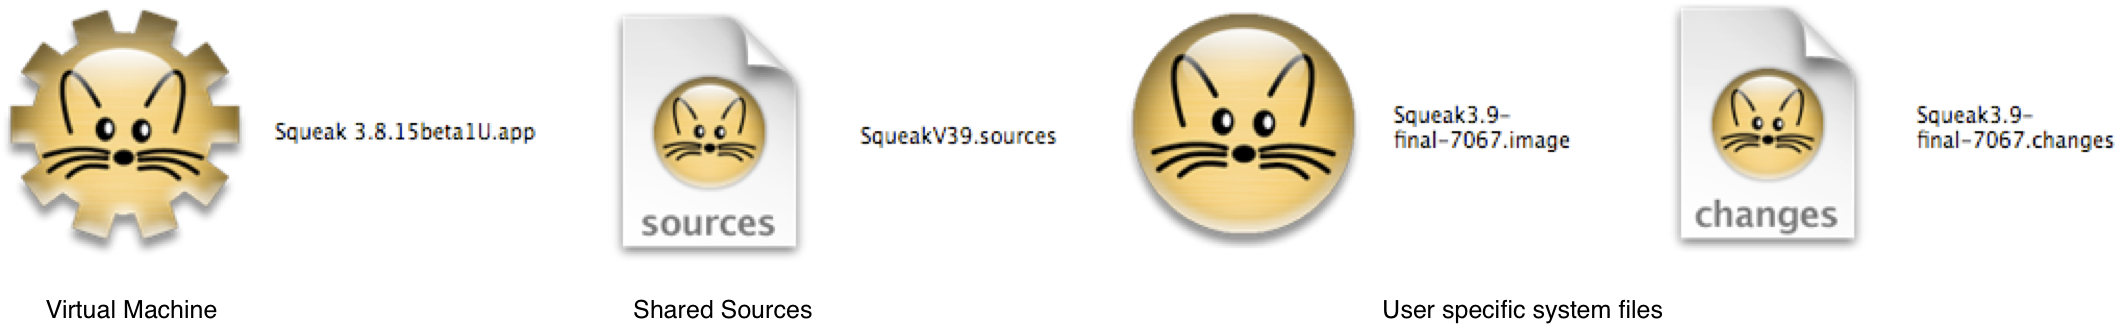
\includegraphics[width=\textwidth]{annotatedDownload}}
\caption{The \sq download files.\label{fig:download}}
\end{figure}

\begin{enumerate}

  \item The \emphind{virtual machine} (VM) is the only part of the system that is different for each operating system and processor.  Pre-compiled virtual machines are available for all the major computing environments.  In \figref{download} we see the VM for the Mac is called \textit{\sq 3.8.15beta1U.app}.

  \item The \emphind{sources} file contains the source code for all of the parts of \sq that don't change very frequently. In \figref{download} it is called \emph{SqueakV39.sources}. Note that the file SqueakV39.sources is only for versions 3.9 and later of \sq. For earlier versions, use a sources file corresponding to the main version \eg \textit{SqueakV3.sources} for versions of \sq from 3.0 up to 3.8.

  \item The current \emph{system \ind{image}} is a snapshot of a running \sq system, frozen in time.  It consists of two files: an \emph{.}\emphind{image} file, which contains the state of all of the objects in the system (including classes and methods, since they are objects too), and a \emph{.}\emphind{changes} file, which contains a log of all of the changes to the source code of the system.
In \figref{download}, we see that we have grabbed the \textit{Squeak3.9-final-7067} image and changes files.
Actually, we will use a slightly different image in this book.
\end{enumerate}

\dothis{Download and install \sq on your computer.
We recommend that you use the standard image provided on the \sq web page.}
\index{download}
\label{sec:sbeImage}

Most of the introductory material in this book will work with any version, so if you already have one installed, you may as well continue to use it.
However, if you notice differences between the appearance or behavior of your system and what is described here, do not be surprised.

As you work in \sq, the \emphind{image} and \emphind{changes} files are modified, so you need to make sure that they are writable.
Always keep these two files together.
Never edit them directly with a text editor, as \sq uses them to store the objects you work with and to log the changes you make to the source code.
It is a good idea to keep a backup copy of the downloaded image and changes files so you can always start from a fresh image and reload your code.

The \emphind{sources} file and the \emphind{VM} can be read-only\,---\,they can be shared between different users.
All of these files can be placed in the same directory, but it is also possible to put the virtual machine and sources file in a separate directory where everyone has access to them.
Do whatever works best for your style of working and your operating system.

\sd{it would be really nice to have a setup and startup section on PC, Mac and Linux}
\ab{I agree entirely; the reason that this is not here is because I could do only the Mac section.  Damien can probably do Windoze.  Perhaps we can ask on the list for a Linux volunteer?}

%-----------------------------------------------------------------
%%{SBESqueakPicture writeTo: './figures/startup.png' frame: (0 @ 0 extent: 900 @ 700) using: [:helper |
%%  helper world color: Color darkGray.
%%  " note: only if you have balloon.png in your image's folder, you'll get the balloon for the startup screen "
%%  ReleaseBuilder openWelcomeWorkspacesWith: ReleaseBuilder getBalloonForm.
%%  PreferenceWizardMorph open.
%%]}
\begin{figure}[htb]
% \centerline {
\includegraphics[width=0.6\textwidth]{download}}
\centerline {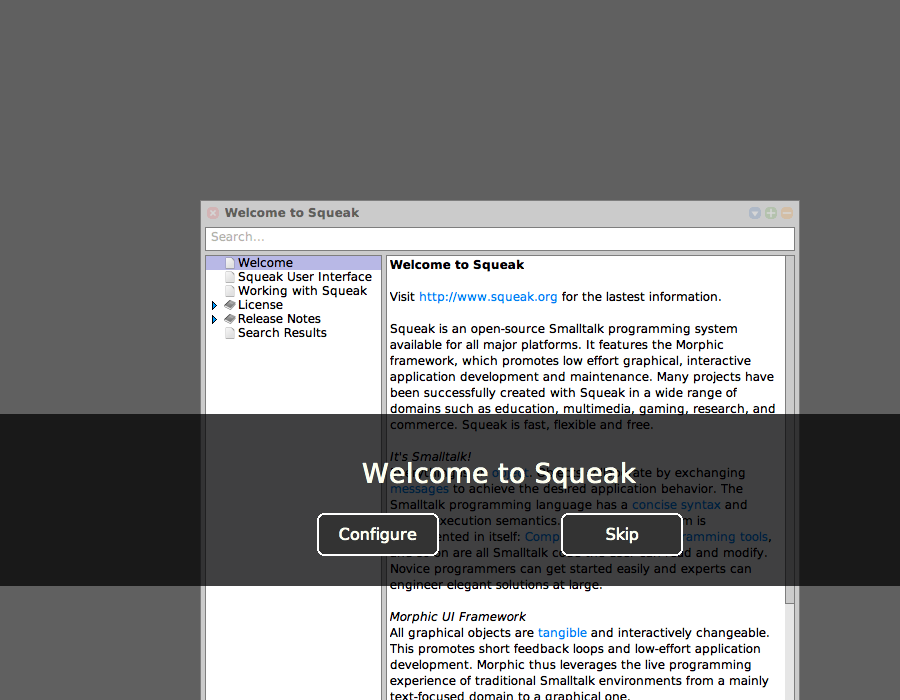
\includegraphics[width=\textwidth]{startup}}
\caption{A fresh \sbe image.\label{fig:startup}}
\end{figure}

\index{launching Squeak}
\paragraph{Launching.} To start \sq, do whatever your operating system expects: drag the \emph{.}\emphind{image} file onto the icon of the virtual machine, or double-click the \emph{.image} file, or  at the command line type the name of the virtual machine followed by the path to the \emph{.image} file. (When you have multiple VMs installed on your machine the operating system may not automatically pick the right one; in this case it is safer to drag and drop the image onto the virtual machine, or to use the command line.)

Once \sq is running, you should see a single large window, possibly containing some open workspace windows (see \figref{startup}). You will also notice that there is a small menu bar at the top. Beyond this one global menu, \sq makes heavy use of context-dependent pop-up menus.

\dothis{Start \sq. You can dismiss any open workspaces by clicking on the {\sf X} in the top left corner of the workspace window.  You can collapse the windows (so that they can be expanded again later) by clicking on the \raisebox{-0.2ex}{{\Large $-$}} in the top-right corner.}

%-----------------------------------------------------------------
\paragraph{First Interaction.}

A good place to get started is the \ind{world menu} shown in \figref{threeButtons:red}. 

\dothis{Click with the mouse on the background of the main window to show the world menu, then choose \menu{open \ldots \go workspace} to create a new workspace.}
%%{SBESqueakPicture writeTo: './figures/worldMenu.png' frame: #morphs using: [:helper |
%%  helper click: helper world at: helper world topCenter + (0 @ 30) buttons: #(left).
%%  helper hand releaseMouseFocus.
%%  helper mouseEnter: (helper menuItemMorphLabeled: 'open...' in: helper world).
%%  helper closeBalloons.
%%]}

%%{SBESqueakPicture writeTo: './figures/yellowButtonMenuOnWorkspace.png' frame: #morphs using: [:helper | | workspace |
%%  workspace := ToolBuilder open: Workspace new.
%%  helper type: 'Time now ' into: workspace.
%%
%%  helper click: workspace at: workspace topCenter + (0 @ 30) buttons: #(right).
%%  helper hand releaseMouseFocus.
%%  helper mouseEnter: (helper menuItemMorphLabeled: 'print it (p)' in: helper world).
%%  helper closeBalloons.
%%]}

%%{SBESqueakPicture writeTo: './figures/morphicHaloOnWorkspace.png' frame: [:rectangle | rectangle outsetBy: 50] using: [:helper | | workspace |
%%	workspace := ToolBuilder open: Workspace new.
%%	helper type: 'Time now ' into: workspace.
%%	helper adjustMorphsArea.
%%	workspace addHalo.
%%]}

\begin{figure}[tbh]
	\centering
	\subfigure[The world menu]{\label{fig:threeButtons:red}%
		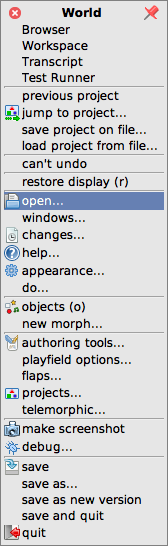
\includegraphics[width=0.2\linewidth]{worldMenu}}\hfill
	\subfigure[The contextual menu]{\label{fig:threeButtons:yellow}%
		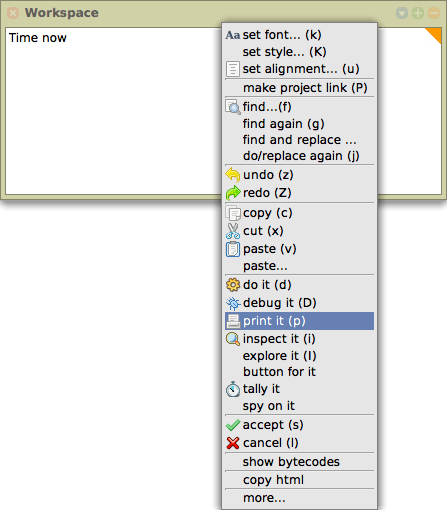
\includegraphics[width=0.25\linewidth]{yellowButtonMenuOnWorkspace}}\hfill
	\subfigure[The morphic halo]{\label{fig:threeButtons:blue}%
		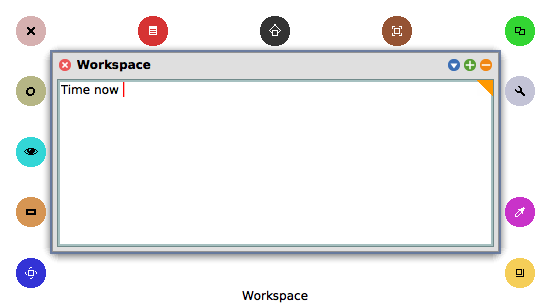
\includegraphics[width=0.25\linewidth]{morphicHaloOnWorkspace}}% these braces needed (else no whitespace at end of line)
	\caption{The world menu (brought up by the red mouse button), a contextual menu (yellow mouse button), and a morphic \subind{Morphic}{halo} (blue mouse button).\label{fig:threeButtons}}
\end{figure}
\index{red button}
\index{yellow button}
\index{blue button}
\seeindex{morphic halo}{Morphic}

% ON: I had to shrink this and move it up to avoid
% it running over the end of the page.
\begin{wrapfigure}[19]{r}{0.25\linewidth}
% The parameters are the number of narrow lines to the right of the figure [19],
% the placement {r} for right, and the width of the figure. Capital R will allow some float.
% Inside the wrapfig environment, linewidth is special --- the width of the figure.
\includegraphics[width=0.95\linewidth]{colouredMouse}
\caption{The author's mouse. Clicking the scroll wheel activates the blue button.}
\label{fig:colouredMouse}
\end{wrapfigure}

\sq was originally designed for a computer with a \ind{three button mouse}.  If your mouse has fewer than three buttons, you will have to press extra keys while clicking the mouse to simulate the extra buttons.

\sq avoids terms like ``left mouse click'' because different computers, mice, keyboards and personal configurations mean that different users will need to press different physical buttons to achieve the same effect.  Instead, the mouse buttons are labeled with colors.  The mouse button that you pressed to get the ``World'' menu is called the \emphind{red button}; it is most often used for selecting items in lists, selecting text, and selecting menu items.
When you start using \sq, it can be surprisingly helpful to actually label your mouse, as shown in \figref{colouredMouse}.\footnote{We will avoid the term ``red-click'' and use ``click'' instead, since this is the default.}

The \emphind{yellow button} is the next most used button; it is used to bring up a contextual menu, that is, a menu that offers different sets of actions depending on where the mouse is pointing; see \figref{threeButtons:yellow}.

\dothis{Type \ct{Time now} in the workspace.
Now click the yellow button in the workspace.
Select \menu{print it}.}

Finally, there is the \emphind{blue button}, which is used to activate the ``morphic \subind{Morphic}{halo}'', an array of handles that are used to perform operations on the on-screen objects themselves, such as rotating them or resizing them; see \figref{threeButtons:blue}. 
If you let the mouse linger over a handle, a help balloon will explain its function.

%%{SBESqueakPicture writeTo: './figures/morphicRotate.png' frame: #morphs using: [:helper | | workspace |
%%  (HaloMorph new createHandleAt: 0 @ 0 color: Color blue iconName: 'Halo-Rot') openInWorld; position: 0 @ 0
%%]}

\dothis{Click the blue button on the workspace.
Grab the \raisebox{-0.4ex}{
\includegraphics[width=1em]{morphicRotate}} handle near the bottom left corner and drag it to rotate the workspace.}

We recommend that right-handed people configure their mouse to put the \ind{red button} on the left side of their mouse, the \ind{yellow button} on the right, and use a clickable scroll wheel, if one is available, for the blue button.  If you don't have a clickable scroll wheel, then you can get the Morphic halo by holding down the \ct{alt} or \ct{option} key while clicking the \ind{red button}.  If you use a Mac without a second mouse button, you can simulate one by holding down the \clover{} key while clicking the mouse.

You can configure your mouse to work the way you want by using the preferences of your operating system and mouse driver.
\sq has some preferences for customising the mouse and the meta keys on your keyboard. You can find the \ind{preference browser} in the \menu{open} item of the \menu{World} menu. 
In the preference browser, the \menu{general} category contains an option \menu{Swap mouse buttons} that switches the yellow and blue functions (see \figref{prefBrowser}).  The \menu{keyboard} category has options to duplicate the various command keys.   

\dothis{Open the preference browser and find the \menu{Swap mouse buttons} option using the search box.}

%%{SBESqueakPicture writeTo: './figures/PreferenceBrowser.png' frame: #morphs using: [:helper | | browser searchText |
%%  searchText := 'swap'.
%%  browser := PreferenceBrowser open.
%%  (browser dependents at: 2) setText: searchText.
%%  browser searchPreferencesFor: searchText.
%%  (helper preferenceButtonMorphLabeled: 'Swap mouse buttons' in: helper world) highlightOn.
%%]}

\begin{figure}[htb]
\ifluluelse
	{\centerline {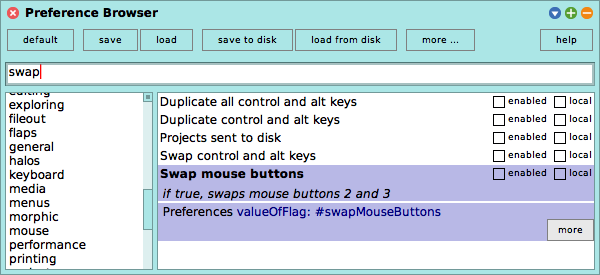
\includegraphics[width=\textwidth]{PreferenceBrowser}}}
	{\centerline {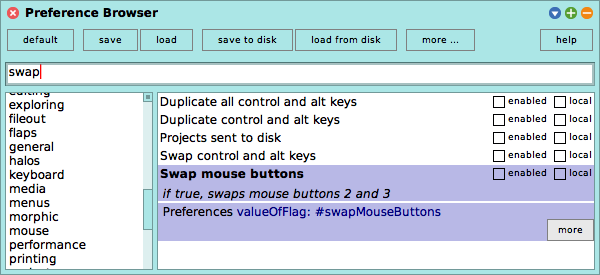
\includegraphics[scale=0.7]{PreferenceBrowser}}}
\caption{The Preference Browser.\label{fig:prefBrowser}}
\end{figure}

%=================================================================
\section{The World menu}
\index{world menu}

\dothis{Click again on the \sq background.}
You will see the \menu{World} menu again.
Most \sq menus are not modal; you can leave them on the screen for as long as you wish by clicking the push pin icon in the top-right corner. Do this. Also, notice that menus appear when you click the mouse, but do not disappear when you release it; they stay visible until you make a selection, or until you click outside of the menu. You can even move the menu around by grabbing its title bar.

The world menu provides you a simple means to access many of the tools that \sq offers.

\dothis{Have a closer look at the \menu{world\go{}open \ldots} menu.}
You will see a list of several of the core tools in \sq, including the system browser (one of many available class browsers) and the workspace.
We will encounter most of them in the coming chapters.

%%{SBESqueakPicture writeTo: './figures/OpenMenu.png' frame: #morphs using: [:helper |
%%  helper click: helper world.
%%  (helper menuItemMorphLabeled: 'open...' in: helper world) invokeWithEvent: nil.
%%  helper closeBalloons.
%%  helper hand releaseMouseFocus.
%%]}

\begin{figure}[htb]
\ifluluelse
	%{\centerline {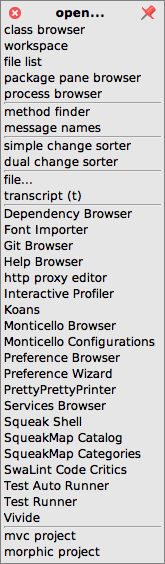
\includegraphics[width=0.3\textwidth]{OpenMenu}}}
	{\centerline {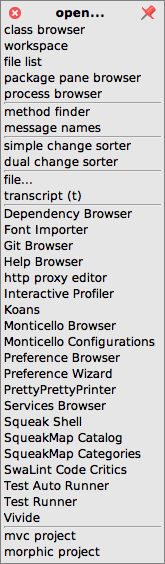
\includegraphics[scale=0.4]{OpenMenu}}}
	{\centerline {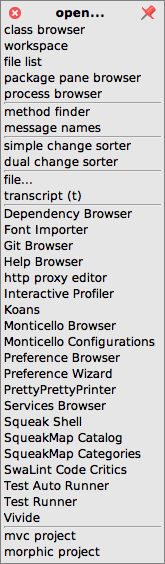
\includegraphics[scale=0.7]{OpenMenu}}}
\caption{The \menu{open \ldots} dialogue of the world menu.\label{fig:openmenu}}
\end{figure}

%=================================================================
\section{Saving, quitting and restarting a \sq session}

\dothis{Bring up the world menu.
Now select \menu{new morph \ldots} and navigate to \menu{from alphabetical list{\go}A-C{\go}BouncingAtomsMorph}.
You now have a morph full of bouncing atoms ``in hand''.
Put the atoms morph down (by clicking) somewhere.}
\index{Morphic}

%%{SBESqueakPicture writeTo: './figures/saveAs.png' frame: #morphs using: [:helper |
%%  helper click: helper world.
%%  
%%  helper
%%    runModal: [(helper menuItemMorphLabeled: 'save as...' in: helper world) invokeWithEvent: nil]
%%    then: [
%%      helper closeBalloons.
%%      helper type: 'SBE' into: (helper morphByExternalName: 'inputText' in: helper world) firstSubmorph firstSubmorph].
%%]}

%%{SBESqueakPicture writeTo: './figures/BouncingAtoms.png' frame: #morphs using: [:helper |
%%  BouncingAtomsMorph new openInWorld
%%]}

\begin{figure}[htb]
\begin{minipage}[b]{0.48\textwidth}
\ifluluelse
	{\centerline{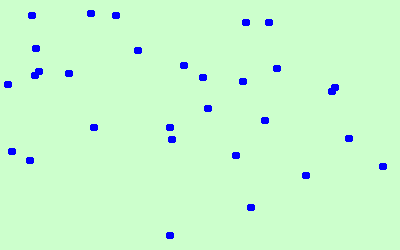
\includegraphics[scale=0.5]{BouncingAtoms}}}
	{\centerline{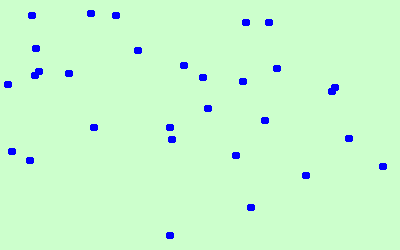
\includegraphics[scale=0.7]{BouncingAtoms}}}
	\caption{An instance of \lct{BouncingAtomsMorph}.\label{fig:bouncingAtoms}}
\end{minipage}
\hfill
\begin{minipage}[b]{0.48\textwidth}
\ifluluelse
	{\centerline {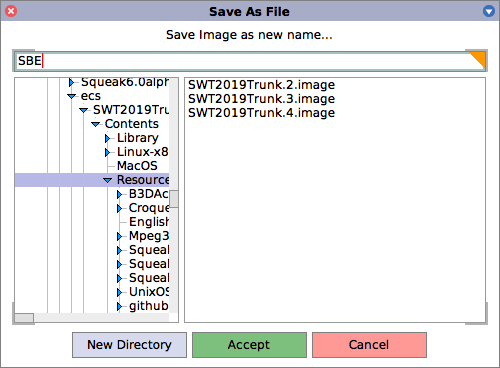
\includegraphics[scale=0.5]{saveAs}}}
	{\centerline {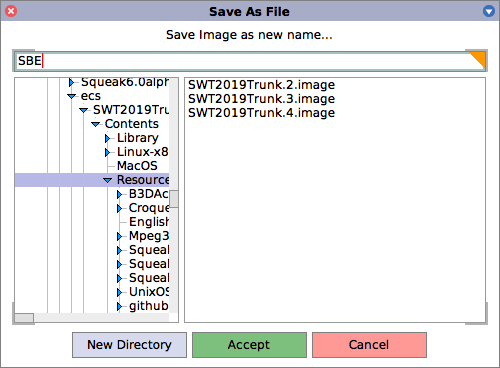
\includegraphics[scale=0.7]{saveAs}}}
	\caption{The \menu{save as \ldots} dialogue.\label{fig:saveas}}
\end{minipage}
\end{figure}

\dothis{Select \menu{World\go{}save as \ldots}, and enter the name ``SBE''.
Now click on the \menu{Accept(s)} button.
Now select \menu{World\go{}save and quit}.}

Now if you go to the location where the original image and changes files were, you will find two new files called ``SBE.\ind{image}'' and ``SBE.\ind{changes}''\footnote{} that represent the working state of the \sq image at the moment before you told \sq to \menu{save and quit}.
If you wish, you can move these two files anywhere that you like on your disk, but if you do so you may (depending on your operating system) need to also move, copy or link to the virtual machine and the \emph{.source} file.

\dothis{Start up \sq from the newly created ``SBE.image'' file.}

Now you should find yourself in precisely the state you were when you quit \sq. The bouncing atoms morph is there again and the atoms continue to move from where they where when you left it.

When you start \sq for the first time, the \sq \ind{virtual machine} loads the image file that you provide. This file contains a snapshot of a large number of objects, including a vast amount of pre-existing code and a large number of programming tools (all of which are objects). As you work with \sq, you will send messages to these objects, you will create new objects, and some of these objects will die and their memory will be reclaimed (\ie garbage-collected).

When you quit \sq, you will normally save a snapshot that contains all of your objects.  If you save normally, you will overwrite your old image file with the new snapshot. Alternatively you may save the image under a new name, as we just did.

In addition to the \emph{.image} file, there is also a \emph{.changes} file.
This file contains a log of all the changes to the source code that you have made using the standard tools.
Most of the time you do not need to worry about this file at all.
As we shall see, however, the \emph{.changes} file can be very useful for recovering from errors, or replaying lost changes.
More about this later!

The image that you have been working with is a descendant of the original \st-80 image created in the late 1970s.
Some of these objects have been around for decades!

The image can be used as a mechanism for storing and managing software projects you are working on.
However, as we shall see later on, there are also tools for managing code and sharing software developed by teams.
For now we will continue by cleaning up the image before we take a look at tools \sq provides.

%%{SBESqueakPicture writeTo: './figures/Tools.png' frame: #morphs using: [:helper |
%%	| thirdWorld workspace worldWindow |
%%	thirdWorld := PasteUpMorph newWorldForProject: nil.
%%	thirdWorld
%%		extent: 750 @ 500;
%%		color: Color white.
%%	Flaps newToolsFlap openInWorld: thirdWorld; showFlap.
%%	Flaps newSqueakFlap openInWorld: thirdWorld.
%%	workspace := ToolBuilder build: (Workspace new
%%		shouldStyle: false;
%%		contents: 'Use the <i>flap</i> on the right to open a tool window.' asTextFromHtml;
%%		yourself).
%%	workspace
%%		setLabel: 'Welcome';
%%		openInWorld: thirdWorld;
%%		center: thirdWorld center.
%%	worldWindow := thirdWorld imageForm asMorph
%%		openInWindowLabeled: 'Squeak by Example'
%%		inWorld: helper world.
%%	worldWindow setStripeColorsFrom: worldWindow defaultColor.
%%]}
\begin{figure}[htb]
\ifluluelse
	{\centerline {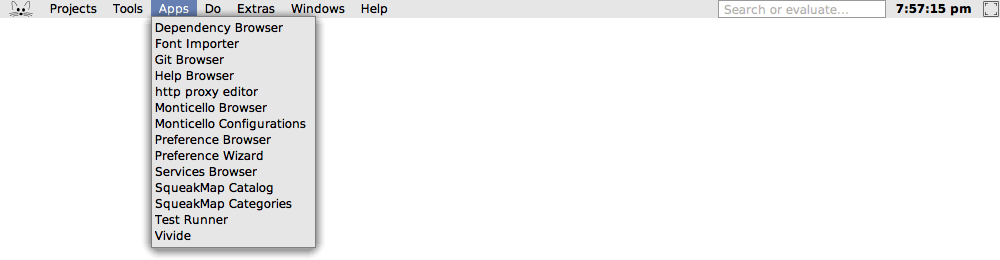
\includegraphics[width=\textwidth]{Tools}}}
	{\centerline {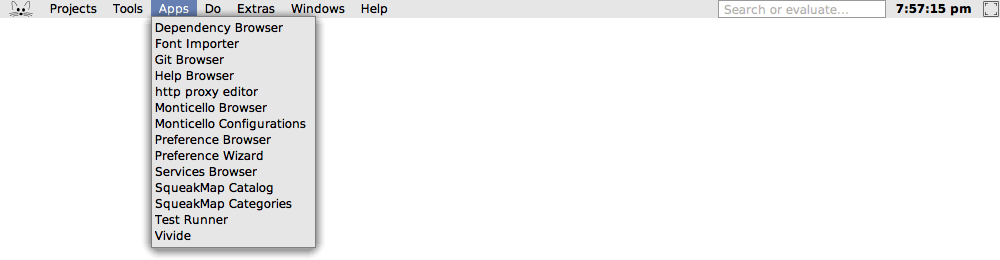
\includegraphics[width=0.8\textwidth]{Tools}}}
\caption{The \sq \toolsflap.\label{fig:tools}}
\end{figure}

%=================================================================
\section{Workspaces and Transcripts}
\label{sec:transcript}

\dothis{Close all open windows. In the menu bar at the top of the \sq environment select \menu{Tools}.}
You will see entries for some of the key tools in \sq (\figref{tools}).
Open a \ind{transcript} and a \ind{workspace}.

\dothis{Position and resize the transcript and workspace windows so that the workspace just overlaps the transcript.}
You can resize windows either by dragging one of the corners, or by blue-clicking the window to bring up the morphic handles, and dragging the yellow, bottom right handle.

At any time only one window is active; it is in front and has its label highlighted (e.g. the workspace window is active in \figref{doit}).

The transcript is an object that is often used for logging system messages.
It is a kind of ``system console''.
Note that the transcript is terribly slow, so if you keep it open and write to it certain operations can become 10 times slower.
In addition the transcript is not thread-safe so you may experience strange problems if multiple objects write concurrently to the transcript.

Workspaces are useful for typing snippets of \st code that you would like to experiment with.
You can also use workspaces simply for typing arbitrary text that you would like to remember, such as to-do lists or instructions for anyone who will use your image.
Workspaces are often used to hold documentation about a captured image, as is the case with the standard image that we downloaded earlier (see \figref{startup}).

\dothis{Type the following text into the workspace:}
\begin{code}{}
Transcript show: 'hello world'; cr.
\end{code}

%%{SBESqueakPicture writeTo: './figures/HelloWorld.png' frame: #morphs using: [:helper | | workspace |
%%  ToolBuilder open: Transcript.
%%  helper world firstSubmorph bounds: (0 @ 120 extent: 450 @ 230).
%%  
%%  workspace := ToolBuilder open: Workspace new.
%%  workspace position: 200 @ 100.
%%  helper type: 'Transcript show: ''hello world''' into: workspace.
%%  
%%  helper hand releaseMouseFocus.
%%  helper closeBalloons.
%%]}

\begin{figure}[htb]
\centerline {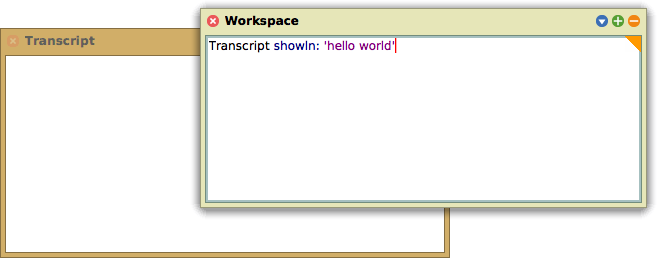
\includegraphics[width=0.6\textwidth]{HelloWorld}}
\caption{Overlapping windows. The workspace is active.\label{fig:helloworld}}
\end{figure}

Try double-clicking in the workspace at various points in the text you have just typed.
Notice how an entire word, entire string, or the whole text is selected, depending on where you click.

\dothis{Select the text you have typed and yellow-click.
Select \menu{do it (d)}.}
Notice how the text ``hello world'' appears in the transcript window
(\figref{doit}).
Do it again.
(The \menu{(d)} in the menu item \menu{do it (d)} tells you that the keyboard shortcut to \emph{do it} is \short{d}. More on this in the next section!)

%%{SBESqueakPicture writeTo: './figures/Doit.png' frame: [:morphsRect | morphsRect withBottom: morphsRect bottom - 150] using: [:helper | | workspace |
%%  ToolBuilder open: Transcript.
%%  Transcript show: 'hello world'.
%%  helper world firstSubmorph bounds: (0 @ 120 extent: 450 @ 230).
%%  
%%  workspace := ToolBuilder open: Workspace new.
%%  workspace position: 200 @ 100.
%%  
%%  helper type: 'Transcript show: ''hello world''' into: workspace.
%%  helper keyStroke: workspace key: $a modifiers: #(cmd).
%%  
%%  helper click: workspace at: workspace topCenter + (0 @ 30) buttons: #(right).
%%  helper hand releaseMouseFocus.
%%  helper mouseEnter: (helper menuItemMorphLabeled: 'do it (d)' in: helper world).
%%  helper closeBalloons.
%%]}
\begin{figure}[htb]
\ifluluelse
	{\centerline {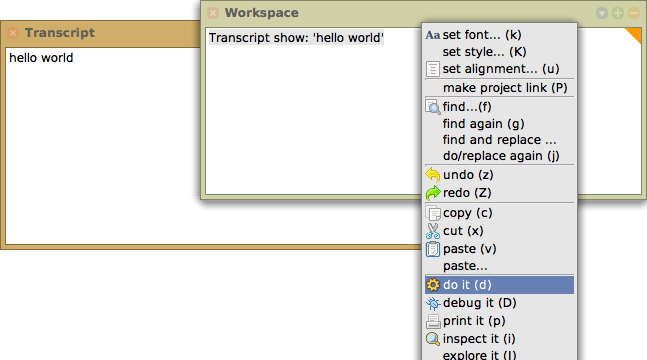
\includegraphics[width=\textwidth]{Doit}}}
	{\centerline {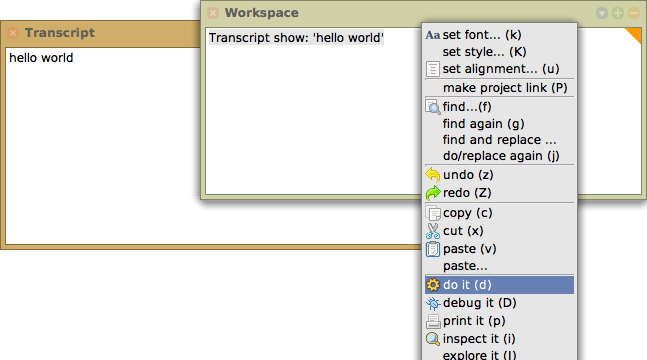
\includegraphics[scale=0.65]{Doit}}}
\caption{``Doing'' an expression\label{fig:doit}}
\end{figure}

You have just evaluated your first \st expression!
You just sent the message \ct{show: 'hello world'} to the \ct{Transcript} object, followed by the message \ct{cr} (carriage return).
The \ct{Transcript} then decided what to do with this message, that is, it looked up its \emph{methods} for handling \ct{show:} and \ct{cr} messages and reacted appropriately.

If you talk to Smalltalkers for a while, you will quickly notice that they generally do not use expressions like ``call an operation'' or ``invoke a method'', but instead they will say ``send a message''.
This reflects the idea that objects are responsible for their own actions. 
You never \emph{tell} an object what to do\,---\,instead you politely \emph{ask} it to do something by sending it a message. 
The object, not you, selects the appropriate method for responding to your message (more about this in \charef{understanding}).


%=================================================================
\section{Keyboard shortcuts}

If you want  to evaluate an expression, you do not always have to bring up the yellow-button menu. Instead, you can use \ind{keyboard shortcuts}. These are the parenthesized expressions in the menu.  Depending on your platform, you may have to press one of the modifier keys (control, alt, command, or meta).
(We will indicate these generically as \short{\emph{key}}.)

\dothis{Evaluate the expression in the workspace again, but using the keyboard shortcut: \short{d}.}
\index{keyboard shortcut!do it}

In addition to \menu{do it}, you will have noticed \menu{print it}, \menu{inspect it} and \menu{explore it}. Let's have a quick look at each of these.

\dothis{Type the expression \ct{3 + 4} into the workspace. Now \menu{do it} with the keyboard shortcut.}

Do not be surprised if you saw nothing happen! What you just did is send the message \ct{+} with argument \ct{4} to the number \ct{3}. Normally the result \ct{7} will have been computed and returned to you, but since the workspace did not know what to do with this answer, it simply threw the answer away.  If you want to see the result, you should \menu{print it} instead. \menu{print it} actually compiles the expression, executes it, sends the message \ct{printString} to the result, and displays the resulting string.

\dothis{Select \ct{3+4} and \menu{print it} (\short{p}).}
This time we see the result we expect (\figref{printit}).
\index{keyboard shortcut!print it}

%%{SBESqueakPicture writeTo: './figures/PrintIt.png' frame: #morphs using: [:helper | | workspace |
%%  workspace := ToolBuilder open: Workspace new.
%%  workspace extent: 277 @ 143.
%%  
%%  helper type: '3 + 4' into: workspace.
%%  helper keyStroke: workspace key: $a modifiers: #(cmd).
%%  helper keyStroke: workspace key: $p modifiers: #(cmd).
%%]}
\begin{figure}[htb]
% \centerline {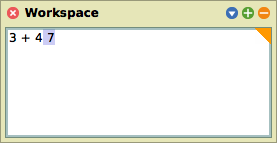
\includegraphics[width=0.4\textwidth]{PrintIt}}
\centerline {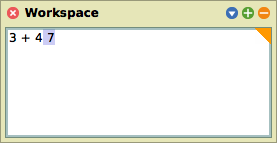
\includegraphics[scale=0.65]{PrintIt}}
\caption{``Print it'' rather than ``do it''. \label{fig:printit}}
\end{figure}

\needlines{3}
\begin{code}{@TEST}
3 + 4 --> 7
\end{code}
\noindent
We use the notation \ct{-->} as a convention in this book to indicate that a particular \sq expression yields a given result when you \menu{print it}.

\dothis{Delete the highlighted text ``\ct{7}'' (\sq should have selected it for you, so you can just press the delete key). Select \ct{3+4} again and this time \menu{inspect it} (\short{i}).}
\noindent
Now you should see a new window, called an \emphind{inspector}, with the heading \ct{SmallInteger: 7} (\figref{inspectit}).
The inspector is an extremely useful tool that will allow you to browse and interact with any object in the system.
The title tells us that \ct{7} is an instance of the class \clsind{SmallInteger}.
The left panel allows us to browse the instance variables of an object, the values of which are shown in the right panel.
The bottom panel can be used to write expressions to send messages to the object.

%%{SBESqueakPicture writeTo: './figures/InspectIt.png' frame: #morphs using: [:helper | | workspace |
%%  workspace := ToolBuilder open: Workspace new.
%%  workspace bounds: (0 @ 30 extent: 277 @ 143).
%%  
%%  helper type: '3 + 4' into: workspace.
%%  helper keyStroke: workspace key: $a modifiers: #(cmd).
%%  helper keyStroke: workspace key: $i modifiers: #(cmd).
%%  (helper windowLabeled: 'SmallInteger.+' asRegex) position: 120 @ 0.
%%]}
\begin{figure}[htb]
\centerline {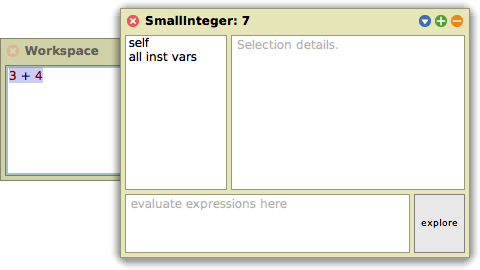
\includegraphics[scale=0.65]{InspectIt}}
\caption{Inspecting an object. \label{fig:inspectit}}
\end{figure}

\dothis{Type \ct{self squared} in the bottom panel of the inspector on \ct{7} and \menu{print it}.}

\needlines{2}
\dothis{Close the inspector. Type the expression \ct{Object} in a workspace and this time \menu{explore it} (\short{I}, uppercased i).}
\index{keyboard shortcut!explore it}
\index{explorer}

This time you should see a window labeled \clsind{Object} containing the text
\mbox{$\triangleright$ \ct{root: Object}}.
Click on the triangle to open it up (\figref{exploreit}).

%%{SBESqueakPicture writeTo: './figures/ExploreIt.png' frame: #morphs using: [:helper |
%%  Object explore
%%]}
\begin{figure}[htb]
\centerline {\includegraphics[scale=0.65]{ExploreIt}}
\caption{Exploring an object. \label{fig:exploreit}}
\end{figure}

The explorer is similar to the inspector, but it offers a tree view of a complex object.
In this case the object we are looking at is the \ct{Object} class.
We can see directly all the information stored in this class, and we can easily navigate to all its parts, e.g. its super class which is stored in \ct{superclass}.

%=================================================================
\section{The System Browser}

The \ind{system browser} is one of the key tools used for programming.
As we shall see, there are several interesting browsers available for \sq, but this is the basic one you will find in any image.
\seeindex{class browser}{system browser}
\seeindex{browser}{system browser}

\dothis{Open a browser by selecting \menu{World \go Browser}, or by selecting \menu{Tools \go Browser} in the world menu bar.}

%%{SBESqueakPicture writeTo: './figures/ClassBrowser2.png' frame: #morphs using: [:helper |
%%	| class selector window codePane |
%%	class := Object. selector := #printString.
%%	Browser fullOnClass: class selector: selector.
%%	window := helper world firstSubmorph.
%%	
%%	Dictionary new
%%		at: class category put: 'System categories';
%%		at: ('\s*' , class) asRegex put: 'Classes';
%%		at: (class categoryForSelector: selector) put: 'Protocols';
%%		at: selector put: 'Methods';
%%		keysAndValuesDo: [:item :description |
%%			(NewBalloonMorph
%%				string: description for: (helper listMorphIncludingMatch: item in: window) owner)
%%					popUp].
%%	codePane := helper textMorphIn: window textMatchedBy: 'printString[\s\S]*' asRegex.
%%	(NewBalloonMorph string: 'name of method' for: codePane)
%%			popUpAt: codePane topLeft + (10 @ 5).
%%	(SBEBalloonMorph string: 'method comment' for: codePane)
%%			popUpTaillessAt: (codePane bounds pointAtFraction: 0.93 @ 0.12).
%%	(SBEBalloonMorph
%%		string: ('code of method\"{1}"' withCRs format: {selector})
%%		for: codePane)
%%			popUpTaillessAt: (codePane bounds pointAtFraction: 1 / 3 @ (1 / 2)).
%%]}
\begin{figure}[htb]
\ifluluelse
	{\centerline {\includegraphics[width=\textwidth]{ClassBrowser2}}}
	{\centerline {\includegraphics[scale=0.7]{ClassBrowser2}}}
\caption{The system browser showing the \ct{printString} method of class \ct{Object}.
\label{fig:classBrowser}}
\end{figure}

We can see a system browser in \figref{classBrowser}.
The title bar indicates that we are browsing the class \clsind{Object}.\footnote{If the browser you have seems to differ from the one described in this book, you may be using an image with a different default browser. See \faqref{omnibrowser}.}

When the browser first opens, all panes are empty except for the leftmost one.
This first pane lists all known \emph{system categories}, which are groups of related classes.
\index{category!system}

\dothis{Click on the category \scatind{Kernel-Objects}.}
This causes the second pane to show a list of all of the classes in the selected category.

\dothis{Select the class \clsind{Object}.}
Now the remaining two panes will be filled with text.
The third pane displays the \emph{method categories} of the currently selected class.
These are convenient groupings of related methods.
If no \ind{method category} is selected you should see all methods in the fourth pane.

\dothis{Select the \protind{printing} category.}
You may have to scroll down to find it.
Now you will see in the fourth pane only methods related to printing.
\index{category!method}
\index{category!message|see method}

\dothis{Select the \mthind{Object}{printString} method.}
Now we see in the bottom pane the source code of the \ct{printString} method, shared by all objects in the system (except those that override it).

%=================================================================
\section{Finding classes}

There are several ways to find a class in \sq.  The first, as we have just seen above, is to know (or guess) what category it is in, and to navigate to it using the browser.
\index{system browser}
\seeindex{system browser!finding classes}{class, finding}
\index{class!finding}

A second way is to send the \ct{browse} message to the class, asking it to open a browser on itself.  Suppose we want to browse the class \clsind{Boolean}.
 
\dothis{Type \ct{Boolean browse} into a workspace and \menu{do it}.}
A browser will open on the Boolean class (\figref{browseBoolean}).
There is also a \ind{keyboard shortcut} \short{b} (browse) that you can use in any tool where you find a class name;
\index{keyboard shortcut!browse it}
select the name and type \short{b}.

\dothis{Use the keyboard shortcut to browse the class \ct{Boolean}.}

%%{SBESqueakPicture writeTo: './figures/Kernel-objects-boolean.png' frame: #morphs using: [:helper | | workspace |
%%  Browser fullOnClass: Boolean
%%]}
\begin{figure}[hbt]
\ifluluelse
	{\centerline {\includegraphics[width=\textwidth]{Kernel-objects-boolean}}}
	{\centerline {\includegraphics[scale=0.7]{Kernel-objects-boolean}}}
\caption{The system browser showing the definition of class Boolean.
\label{fig:browseBoolean}}
\end{figure}

Notice that when the \ct{Boolean} class is selected but no method category or method is selected, the bottom pane automatically shows the \emph{class definition}
(\figref{browseBoolean}).
This is nothing more than an ordinary \st message that is sent to the parent class, asking it to create a subclass.
Here we see that the class \ct{Object} is being asked to create a subclass named \ct{Boolean} with no instance variables, class variables or ``pool dictionaries'', and to put the class \ct{Boolean} in the \scatind{Kernel-Objects} category.

If you want to see further information on the class, you can click on the \button{?} at the bottom of the class pane. This opens the \subind{class}{comment} in a dedicated pane.

\ab{I thought that this was supposed to be a \emph{Quick} tour!  And here we are describing a tool that I have used maybe twice in 10 years!   In any case, this description should be deferred to the \textbf{Environment} chapter}
\on{I don't see why.  I use the hierarchy browser a lot!  I think it is really useful to know from the beginning, to help you find your through the hierarchy.}
If you would like to explore \sq's inheritance hierarchy, the \emphind{hierarchy browser} can help you.  
This can be useful if you are looking for an unknown subclass or superclass of a known class.
The hierarchy browser is like the system browser, except that the list of classes is arranged as an indented tree mirroring the inheritance hierarchy.

\dothis{Click on \button{hierarchy} in the browser while the class \ct{Boolean} is selected.}
\noindent
This will open a hierarchy browser showing the superclasses and subclasses of \clsind{Boolean}.
% (\figref{booleanhierarchybrowser}).

%%{SBESqueakPicture writeTo: './figures/BooleanHierarchyBrowser.png' frame: [:morphsRect | morphsRect] using: [:helper | | browser browserMorph b_morph |
%%  browser := HierarchyBrowser new.
%%  browser setClass: Boolean.
%%  browser buildDefaultBrowserWith: ToolBuilder default.
%%  b_morph := ToolBuilder open: browser.
%%  b_morph submorphs ninth repositionBy: (0@60).
%%  helper closeBalloons.
%%]}

Navigate to the immediate superclass and subclasses of \ct{Boolean}.

Often, the fastest way to find a class is to search for it by name.  For example, suppose that you are looking for some unknown class that represents dates and times.

\dothis{Put the mouse in the system category pane of the system browser and type \short{f}, or select \menu{find class \ldots (f)} from the yellow-button menu.  Type ``time'' in the dialog box.} 
\noindent
You will be presented with a list of classes whose names contain ``time'' (see \figref{findit}).  Choose one, say, \ct{Time}, and the browser will show it.
\index{keyboard shortcut!find ...}

%%{SBESqueakPicture writeTo: './figures/FindIt.png' frame: #morphs using: [:helper | | browser |
%%  browser := ToolBuilder open: Browser.
%%  browser position: 0 @ 0.
%%  
%%  helper
%%    runModal: [helper keyStroke: browser submorphs sixth key: $f modifiers: #(cmd)]
%%    then: [helper dialogWindow position: 60 asPoint]
%%]}

%%{SBESqueakPicture writeTo: './figures/TimeClasses.png' frame: #morphs using: [:helper | | browser |
%%  browser := ToolBuilder open: Browser.
%%  browser position: 0 @ 0.
%%  
%%  helper
%%    runModal: [helper keyStroke: browser submorphs sixth key: $f modifiers: #(cmd)]
%%    then: [
%%      helper dialogWindow position: 60 asPoint.
%%      helper type: 'time' into: (helper morphByExternalName: 'searchText' in: helper world).
%%      helper closeBalloons.
%%    ].
%%  
%%]}

\begin{figure}[hbt]
\centerline{
\ifluluelse{
	\includegraphics[width=0.5\textwidth]{FindIt}
	\hspace{1cm}
	\includegraphics[width=0.4\textwidth]{TimeClasses}
}{
	\includegraphics[width=0.4\textwidth]{FindIt}
	\hspace{1cm}
	\includegraphics[width=0.3\textwidth]{TimeClasses}
}
}
\caption{Searching for a class by name.
\label{fig:findit}}
\end{figure}

%=================================================================
\section{Finding methods}
\label{sec:quick:methodFinder}

Sometimes you can guess the name of a method, or at least part of the name of a method, more easily than the name of a class.  For example, if you are interested in the current time, you might expect that there would be a method called ``now'', or containing ``now'' as a substring.   But where might it be?
The \emphind{method finder} can help you.
\seeindex{system browser!finding methods}{method, finding}
\index{method!finding}

\dothis{Select \menu{Tools \go Method Finder} in the menu bar at the top or open the world menu and select \menu{open\ldots \go method finder}.
Type ``now'' in the top left pane, and \menu{accept} it (or just press the \textsc{return} key).}
The method finder will display a list of all the method names that contain the substring ``now''.  
To scroll to \ct{now} itself, move the cursor to the list and type ``\ct{n}''; this trick works in all scrolling windows.  Select ``now'' and the right-hand pane shows you the three classes that define a method with this name, as shown in \figref{MethodFinder}.  Selecting any one of them will open a browser on it.

%%{SBESqueakPicture writeTo: './figures/methodFinder-now.png' frame: #morphs using: [:helper |
%%	| window inputField hitList |
%%	window := ToolBuilder open: SelectorBrowser new.
%%	inputField := (window rootMorphsAt: window topLeft + 30) first.
%%	hitList := (window rootMorphsAt: inputField bottomLeft + 30) first.
%%	helper
%%		mouseEnter: inputField;
%%		type: 'now' into: inputField;
%%		keyStroke: inputField key: $s modifiers: #(cmd).
%%	['now' matches: hitList selection] whileFalse: [
%%		helper keyStroke: hitList key: Character arrowDown].
%%	4 "scroll the selection nicely into view"
%%		timesRepeat: [helper keyStroke: hitList key: Character arrowDown];
%%		timesRepeat: [helper keyStroke: hitList key: Character arrowUp]
%%]}

\begin{figure}[hbt]
\centerline {\includegraphics[scale=0.6]{methodFinder-now}}
\caption{The method finder showing three classes that define a method named \ct{now}.
\label{fig:MethodFinder}}
\end{figure}

At other times you may have a good idea that a method exists, but will have no idea what it might be called.
The method finder can still help!  For example, suppose that you would like to find a method that turns a string into upper case, for example, it would translate \ct{'eureka'} into \ct{'EUREKA'}.

\dothis{Type \ct{'eureka' . 'EUREKA'} into the method finder and press
  the \textsc{return} key, as shown in
  \figref{methodFinder-example1}.}
\noindent
The method finder will suggest a method that does what you want.

An asterisk at the beginning of a line in the right pane of the method finder indicates that this method is the one that was actually used to obtain the requested result. 
So, the asterisk in front of \ct{String asUppercase} lets us know that the method \mthind{String}{asUppercase} defined on the class \clsind{String} was executed and returned the result we wanted. The methods that do not have an asterisk are just the other methods that have the same name as the ones that returned the expected result. So \cmind{Character}{asUppercase} was not executed on our example, because \ct{'eureka'} is not a \clsind{Character} object.

%%{SBESqueakPicture writeTo: './figures/MethodFinder-example1.png' frame: #morphs using: [:helper |
%%	| window inputField hitList |
%%	window := ToolBuilder open: SelectorBrowser.
%%	window extent: 500 @ 210.
%%	inputField := (window rootMorphsAt: window topLeft + 30) first.
%%	hitList := (window rootMorphsAt: inputField bottomLeft + 30) first.
%%	helper
%%		mouseEnter: inputField;
%%		type: '''eureka''. ''EUREKA''' into: inputField;
%%		keyStroke: inputField key: $s modifiers: #(cmd).
%%	helper click: hitList at: hitList topLeft + 10 buttons: #(left)
%%]}
\begin{figure}[hbt]
\ifluluelse
	{\centerline {\includegraphics[width=0.9\textwidth]{MethodFinder-example1}}}
	{\centerline {\includegraphics[scale=0.7]{MethodFinder-example1}}}
\caption{Finding a method by example.
\label{fig:methodFinder-example1}}
\end{figure}

You can also use the method finder for methods with arguments; for example, if you are looking for a method that will find the greatest common factor of two integers, you might try \ct{25. 35. 5} as an example.  You can also give the method finder multiple examples to narrow the search space; the help text in the bottom pane explains more.

There is yet another way to find both, methods and classes. In the top right corner of the menu bar at the top you can find a pane saying ``Search or evaluate\ldots''. This pane provides you a global search; you can activate it from everywhere via \short{0}. When you try previous searches for the class \ct{Time} or the method \ct{now} you will see that the search directly opens a browser for the class or the methods.

%=================================================================
\section{Defining a new method}

\sq provides many more interesting tools, such as the test runner and the debugger. In order to illustrate you how these are typically used while programming in \sq, we will show you how you can make use of them while defining a new method.

The advent of \ind{Test Driven Development}\cite{Beck03a} has changed the way that we write code.  
The idea behind Test Driven Development, also called TDD or Behavior Driven Development, is that we write a test that defines the desired behavior of our code \emph{before} we write the code itself.
Only then do we write the code that satisfies the test.
\seeindex{Behavior Driven Development}{Test Driven Development}

Suppose that our assignment is to write a method that ``says something loudly and with emphasis''.  What exactly could that mean?  What would be a good name for such a method?  How can we make sure  that programmers who may have to maintain our method in the future have an unambiguous description of what it should do?   We can answer all of these questions by giving an example:

\begin{quote}
When we send the message \ct{shout} to the string ``Don't panic'' the result should be ``DON'T PANIC!''.
\end{quote}

\noindent
To make this example into something that the system can use, we turn it into a test method:
\index{testing}
\index{SUnit}

\needlines{3}
\begin{method}[testShout]{A test for a shout method}
testShout
	self assert: ('Don''t panic' shout = 'DON''T PANICBANG')
\end{method} % BANG is the escape for !

How do we create a new method in \sq?   First, we have to decide which class the method should belong to.
In this case, the \ct{shout} method that we are testing will go in class \clsind{String}, so the corresponding test will, by convention, go in a class called \clsind{StringTest}.

%%{SBESqueakPicture writeTo: './figures/StringTest-newMethodTemplate.png' frame: #morphs using: [:helper |
%%  Browser fullOnClass: StringTest category: #'tests - converting'.
%%  helper click: helper world firstSubmorph firstSubmorph firstSubmorph.
%%  helper click: helper world firstSubmorph firstSubmorph firstSubmorph.
%%]}


\begin{figure}[hbt]
\ifluluelse
	{\centerline {\includegraphics[width=\textwidth]{StringTest-newMethodTemplate}}}
	{\centerline {\includegraphics[width=0.7\textwidth]{StringTest-newMethodTemplate}}}
\caption{The new method template in class \ct{StringTest}.
\label{fig:newMethodTemplate}}
\end{figure}

\dothis{Open a browser on the class \ct{StringTest}, and select an appropriate message category for our method, in this case \menu{tests - converting}, as shown in \figref{newMethodTemplate}.
The highlighted text in the bottom pane is a template that reminds you what a \st method looks like.
Delete this and enter the code from  \mthref{testShout}.}
Once you have typed the text into the browser, notice that the bottom pane is outlined in red.  This is a reminder that the pane contains unsaved changes.
So select \menu{accept (s)} from the yellow-button menu in the bottom pane, or just type \short{s}, to compile and save your method.
\index{keyboard shortcuts}
\index{keyboard shortcut!accept}
\seeindex{accept it}{keyboard shortcut, accept}

Because there is as yet no method called \ct{shout}, the browser will ask you to confirm that this is the name that you really want\,---\,and it will suggest some other names that you might have intended (\figref{testShoutConfirm}).
This can be quite useful if you have merely made a typing mistake, but in this case, we really \emph{do} mean \ct{shout}, since that is the method we are about to create, so we have to confirm this by selecting the first option from the menu of choices, as shown in \figref{testShoutConfirm}. 

%%{SBESqueakPicture writeTo: './figures/testShoutConfirm.png' frame: #morphs using: [:helper | | browser textField |
%%  Browser fullOnClass: StringTest selector: #testCapitalized.
%%  textField := helper world firstSubmorph firstSubmorph firstSubmorph.
%%  helper click: textField.
%%  helper keyStroke: textField key: $a modifiers: #(cmd).
%%  (Symbol classPool at: #SymbolTable) remove: 'shout' ifAbsent: [].
%%  (Symbol classPool at: #NewSymbols) remove: 'shout' ifAbsent: [].
%%  helper type: 'testShout\\    self assert: (''Don''''t panic'' shout = ''DON''''T PANIC!'')' withCRs into: textField.
%%  helper runModal: [helper keyStroke: textField key: $s modifiers: #(cmd)] then: [helper dialogWindow position: 500 @ 40]
%%]}

\begin{figure}[hbt]
\ifluluelse
	{\centerline {\includegraphics[width=\textwidth]{testShoutConfirm}}}
	{\centerline {\includegraphics[scale=0.7]{testShoutConfirm}}}
\caption{Accepting the testShout method class \ct{StringTest}.
\label{fig:testShoutConfirm}}
\end{figure}

\dothis{Run your newly created test: open the \ind{SUnit} \emphind{TestRunner}, either by dragging it from the \toolsflapind, or by selecting \menu{World \go open... \go Test Runner}.}

The leftmost two panes are a bit like the top panes in the system browser.  The left pane contains a list of system categories, but it's restricted to those categories that contain test classes.

\dothis{Select \scat{CollectionsTests-Text} and the pane to the right will show all of the test classes in that category, which includes the class \ct{StringTest}.  The names of the classes are already selected, so click \menu{Run Selected} to run all these tests.}

%%{SBESqueakPicture writeTo: './figures/testRunnerOnStringTest.png' frame: #morphs using: [:helper |
%%  [
%%  StringTest compile: 'testShout self assert: false'.
%%  testRunner := (ToolBuilder open: TestRunner new) model.
%%  categoryIndex := testRunner categoryList indexOf: 'CollectionsTests-Text'.
%%  testRunner categorySelected: categoryIndex.
%%  testRunner categoryAt: categoryIndex put: true.
%%  testRunner selectNoClasses.
%%  testRunner classAt: (testRunner classList findFirst: [:s | s beginsWith: 'StringTest']) put: true.
%%  testRunner runAll] ensure: [StringTest removeSelector: #testShout]
%%]}

\begin{figure}[hbt]
\ifluluelse
	{\centerline {\includegraphics[width=\textwidth]{testRunnerOnStringTest}}}
	{\centerline {\includegraphics[scale=0.5]{testRunnerOnStringTest}}}
\caption{Running the String tests.
\label{fig:testRunnerTestShout}}
\end{figure}

You should see a message like that shown in \figref{testRunnerTestShout}, which indicates that there was an error in running the tests.  The list of tests that gave rise to errors is shown in the bottom right pane; as you can see, \ct{StringTest>>>#testShout} is the culprit.
(Note that \ct{StringTest>>#testShout} is the Smalltalk way of identifying the \mthind{StringTest}{testShout} method of the \ct{StringTest} class.)
If you click on that line of text, the erroneous test will run again, this time in such a way that you see the error happen: ``\ct{MessageNotUnderstood: ByteString>>>shout}''.
\seeindex{\ct{>>}}{Behavior, \ct{>>}}
\cmindex{Behavior}{>>}

The window that opens with the error message is the \st debugger (see \figref{predebugger}).
\ab{Well, it's actually the \emph{pre-}debugger.  Does this matter?}\damien{I don't think it's important at this point.}
We will look at the \ind{debugger} and how to use it in \charef{env}.

%%{SBESqueakPicture writeTo: './figures/Predebugger.png' frame: #morphs using: [:helper |
%%	helper restoreMethods: ((String lookupSelector: #shout) ifNotNil: [{String>>#shout}] ifNil: [#()]) after: [
%%		String removeSelector: #shout.
%%		helper runModal: [StringTest new testShout].
%%	]
%%]}.
\begin{figure}[hbt]
\ifluluelse
	{\centerline {\includegraphics[width=\textwidth]{Predebugger}}}
	{\centerline {\includegraphics[scale=0.7]{Predebugger}}}
\caption{The (pre-)debugger.}
\label{fig:predebugger}
\end{figure}

The error is, of course, exactly what we expected:  running the test generates an error because we haven't yet written a method that tells strings how to \ct{shout}.  
Nevertheless, it's good practice to make sure that the test fails because this confirms that we have set up the testing machinery correctly and that the new test is actually being run.
Once you have seen the error, you can \button{Abandon} the running test, which will close the debugger window.
Note that often with Smalltalk you can define the missing method using the \button{Create} button, edit the newly-created method in the debugger, and then \button{Proceed} with the test.

Now let's define the method that will make the test succeed!

\dothis{Select class \clsind{String} in the system browser, select the \menu{converting} category, type the text in \mthref{shout} over the method creation template, and \menu{accept} it.}
\begin{method}[shout]{The shout method}
shout
	^ self asUppercase, 'BANG'
\end{method}

The comma is the string concatenation operation, so the body of this method appends an exclamation mark to an upper-case version of whatever \ct{String} object the \ct{shout} message was sent to.
The \ct{^} tells \sq that the expression that follows is the answer to be returned from the method, in this case the new concatenated string.
\seeindex{comma}{Collection, comma operator}
\index{Collection!comma operator}

Does this method work?  Let's run the tests and see.

\dothis{Click on \menu{Run Selected} again in the test runner, and this time you should see a green bar and text indicating that all of the tests ran with no failures and no errors.}
When you get to a green bar\footnotemark, it's a good idea to save your work and take a break.  
So do that right now!
\footnotetext{Actually, you might not get a green bar since some images contains tests for bugs that still need to be fixed.
Don't worry about this.
\Squeak is constantly evolving.
%:PROBLEM --- StringTest has a broken test!
% ON: There is a broken test in \ct{StringTest>>>\#testIndexOf}!
}

%%{SBESqueakPicture writeTo: './figures/String-Shout.png' frame: #morphs using: [:helper |
%%  String compile: 'shout\\    ^ self asUppercase, ''!''' withCRs classified: 'converting'.
%%  ToolSet browse: String selector: #shout
%%]}
\begin{figure}[hbt]
\ifluluelse
	{\centerline{\includegraphics[width=\textwidth]{String-Shout}}}
	{\centerline{\includegraphics[scale=0.7]{String-Shout}}}
\caption{The \ct{shout} method defined on class \ct{String}.
\label{fig:String-shout}}
\end{figure}

%=================================================================
\section{Chapter summary}
This chapter has introduced you to the \sq environment and shown you how to use some of the major tools, such as the system browser, the method finder, and the test runner.   You have also seen a little of \sq's syntax, even though you may not understand it all yet.

\begin{itemize}
  \item A running \sq system consists of a \emph{virtual machine}, a \emph{sources} file, and \emph{image} and \emph{changes} files. Only these last two change, as they record a snapshot of the running system.
  \item When you start a \sq image, you will find yourself in exactly the same state\,---\,with the same running objects\,---\,that you had when you last saved that image.
  \item \sq is designed to work with a three-button mouse. The buttons are known as the \emph{red}, the \emph{yellow} and the \emph{blue} buttons. If you don't have a three-button mouse, you can use modifier keys to obtain the same effect.
  \item You use the \ind{red button} on the \sq background to bring up the \emph{World menu} and launch various tools. You can also launch tools from the \toolsflapind at the right of the \sq screen.
  \item A \emph{workspace} is a tool for writing and evaluating snippets of code. You can also use it to store arbitrary text.
  \item You can use \ind{keyboard shortcuts} on text in the workspace, or any other tool, to evaluate code. The most important of these are \menu{do it} (\short{d}), \menu{print it} (\short{p}), \menu{inspect it} (\short{i}), \menu{explore it} (\short{I}) and \menu{browse it} (\short{b}).
  \item The \emph{system browser} is the main tool for browsing \sq code, and for developing new code.
  \item The \emph{test runner} is a tool for running unit tests. It also supports Test Driven Development.
\end{itemize}

%=================================================================
\ifx\wholebook\relax\else 
   \bibliographystyle{jurabib}
   \nobibliography{scg}
   \end{document}
\fi
%=================================================================

%%% Local Variables:
%%% coding: utf-8
%%% mode: latex
%%% TeX-master: t
%%% TeX-PDF-mode: t
%%% ispell-local-dictionary: "english"
%%% End:
